\chapter{Application: Query Log Compression for Workload Analytics}
\label{chapter:querylogsummarization}

\section{Introduction}
% !TEX root = ../paper.tex
Automated analysis of database access logs is critical for solving a wide range of problems, from database performance tuning~\cite{DBLP:conf/sigmod/BrunoC05}, to compliance validation~\cite{DBLP:conf/icalp/Dwork06}, and query recommendation~\cite{DBLP:journals/debu/ChatzopoulouEKMPV11}. 
For example, the Peloton self-tuning database~\cite{DBLP:conf/cidr/PavloAALLMMMPQS17} searches for optimal configurations by repeatedly simulating database performance based on statistical properties of historical queries.
Unfortunately, query logs for production databases can grow to be large ---
A recent study of queries at a major US bank for a period of 19 hours found nearly 17 million SQL queries and over 60 million stored procedure executions~\cite{DBLP:conf/www/KulLXCCKU16} --- and computing these properties from the log itself is slow.

Tracking only a sample of these queries is not sufficient, as rare queries can disproportionately affect database performance, for example, if they benefit from an otherwise unnecessary index.
Rather, we need a compressed \emph{summary} of the log on which we can compute aggregate statistical properties.
The problems of compression and summarization have been studied extensively (e.g.,~\cite{DBLP:journals/tit/ZivL77,DBLP:journals/tit/ZivL78,4051119,lee1999learning,DBLP:reference/stat/Jolliffe11,DBLP:journals/cacm/Blei12,DBLP:conf/acl/WangZLG09,DBLP:journals/ai/KnightM02}). 
However, these schemes either require the use of heavyweight inference to desired statistical measures, or produce unnecessarily large encodings.

In this chapter, we adapt ideas from pattern mining and summarization~\cite{DBLP:journals/tkdd/MampaeyVT12,DBLP:journals/pvldb/GebalyAGKS14} to propose a middle-ground: \systemnameone, a summarization scheme that facilitates efficient (both in terms of storage and time) approximation of workload statistics.
By adjusting a tunable parameter in \systemnameone, users can choose to obtain a high-fidelity, albeit large summary, or obtain a more compact summary with lower fidelity.
Constructing the summary that best balances compactness and fidelity is challenging, as the search space of candidate summaries is combinatorially large~\cite{DBLP:journals/tkdd/MampaeyVT12,DBLP:journals/pvldb/GebalyAGKS14}.
\systemnameone offers a new approach to summary construction that avoids searching this space, making inexpensive, accurate computation of aggregate workload statistics possible.
As a secondary benefit, the resulting summaries are also human-interpretable.

\systemnameone does not admit closed-form solutions to classical fidelity measures like information loss, so an alternative called \emph{\errorname} is proposed.
A combination of analytical and experimental evidence will be shown that \errorname is highly correlated with several classical measures of encoding fidelity.

\systemnameone-compressed data relies on a codebook of structural elements like \texttt{SELECT} items, \texttt{FROM} tables, or conjunctive \texttt{WHERE} clauses~\cite{DBLP:journals/kais/AligonGMRT14}.
This codebook provides a bi-directional mapping from SQL queries to a bit-vector encoding, reducing the compression problem to one of compactly encoding a collection of feature-vectors.
The problem is further simplified by observing that a common theme in use cases like automated performance tuning or query recommendation is the need for predominantly aggregate workload statistics.
As these are order-independent, we are able to focus exclusively on compactly representing \emph{bags} of feature-vectors.

\systemnameone works by identifying groups of co-occurring structural elements that we call patterns.  
A family of \emph{pattern encodings} of access logs is defined, which map patterns to their frequencies in the log.
For pattern encodings, two idealized measures of fidelity are considered: 
(1) Ambiguity, which measures how much room the encoding leaves for interpretation; and 
(2) Deviation, which measures how reliably the encoding approximates the original log.
Neither Ambiguity nor Deviation can be computed efficiently for pattern encodings.
Hence a measure called \emph{\errorname} is proposed that is efficiently computable and that closely tracks both Ambiguity and Deviation.

In general, the size of the encoding is inversely related with \errorname: The more detailed the encoding, the more faithfully it represents the original log.
Thus, log compression may be defined as a search over the space of pattern-based encodings to identify the one that best trades off between these two properties.
Unfortunately, searching for such an ideal encoding from the space can be computationally expensive~\cite{DBLP:journals/tkdd/MampaeyVT12,DBLP:journals/pvldb/GebalyAGKS14}.
To overcome this limitation, the search space is reduced by first clustering entries in the log and then encoding each cluster separately, an approach that we call \textit{pattern mixture encoding}.
Finally I identify a simple approach for encoding individual clusters that we call \textit{naive mixture encodings}, and show experimentally that it produces results competitive with more general techniques for log compression and summarization.

Concretely, in this chapter I make the following contributions:
(1) I define two families of compression for query logs: pattern and pattern mixture, 
(2) I define a computationally efficient measure, \errorname, and demonstrate that it is a close approximation of Ambiguity and Deviation (two commonly used measures),
(3) I propose a clustering-based approach to efficiently search for naive mixture encodings, and show how these encodings can be further optimized, and, 
(4) I experimentally validate \systemnameone and show that it produces more precise encodings, faster than several state-of-the-art pattern encoding algorithms.

\tinysection{Roadmap}
This chapter is organized as follows: Section~\ref{sec:problemdefinition} formally defines the log compression problem and the summary representation;
Section~\ref{sec:analyzingsummaries} then defines information loss of the summaries;
Section~\ref{sec:practicalrepresentativeness} explains the difficulty in computing classical loss measures and provides a practical alternative;
Section~\ref{sec:patternmixtureencodings} motivates data partitioning and generalizes the practical loss measure to partitioned data;
Section~\ref{sec:constructingencodings} then introduces the proposed \systemnameone compression scheme;
Section~\ref{sec:experiments} empirically validates the practical loss measure and evaluates the effectiveness of \systemnameone by comparing it with two state-of-the-art summarization methods;
Section~\ref{sec:evaluatingalternativeapplications} further evaluates \systemnameone under applications of comparison methods.

\section{Problem Definition}
\label{sec:problemdefinition}
% !TEX root = ../paper.tex
In this section, we introduce and formally define the log compression problem.
We begin by exploring several applications that need to repeatedly analyze query logs.

\tinysection{Index Selection}
Selecting an appropriate set of indexes requires trading off between update costs, access costs, and limitations on available storage space.
Existing strategies for selecting a near-optimal set of indexes typically repeatedly simulate database performance under different combinations of indexes, which in turn requires repeatedly estimating the frequency of specific predicates in the workload.
%For example, if \lstinline{status = ?} occurs in $90\%$ of the queries in a workload, a hash index on \lstinline{status} is beneficial.

\tinysection{Materialized View Selection}
The results of joins or highly selective selection predicates are good candidates for materialization when they appear frequently in the workload.  
Like index selection, view selection is a non-convex optimization problem, typically requiring repeated simulation, which in turn requires repeated frequency estimation over the workload.

\tinysection{Online Database Monitoring}
In production settings, it is common to monitor databases for atypical usage patterns that could indicate a serious bug or security threat.
When query logs are monitored, it is often done retrospectively, some hours after-the-fact~\cite{DBLP:conf/www/KulLXCCKU16}.  
To support real-time monitoring it is necessary to quickly compute the frequency of a particular class of queries in the system's typical workload.

\smallskip

In each case, the application's interactions with the log amount to counting queries that have specific features: selection predicates, joins, or similar.

\subsection{Preliminaries and Notation}
\label{sec:notation}
Let $L$ be a log, or a finite collection of queries $\vec q \in L$.
We write $f \in \vec q$ to indicate that $\vec q$ has some \emph{feature} $f$, such as a specific predicate or table in its \lstinline{FROM} clause.
We assume (1) that the universe of features in both a log and a query is enumerable and finite, (2) that the features are selected to suit specific applications and (3) optionally that a query is isomorphic to its feature set (motivated in Section~\ref{sec:communicatinginformationcontent}).  
We outline one approach to extracting features that satisfies all three assumptions below.
We abuse syntax and write $\vec q$ to denote both the query itself, as well as the set of its features.  

Let $\pattern$ denote some set of features $f \in \pattern$.
We write these sets using vector notation: $\pattern=(x_1,\ldots,x_n)$ where $n$ is the number of distinct features in the entire log and $x_i$ indicates the presence (absence) of $i$th feature with a 1 (resp., 0).  
For any two patterns $\pattern$, $\pattern'$, we say that $\pattern'$ \emph{is contained} or \emph{appears} in $\pattern$ if $\pattern' \subseteq \pattern$, or equivalently if $\forall i,\, x'_i\leq x_i$.  
%Equivalently, with $\pattern=(x_1,\ldots,x_n)$ and $\pattern'=(x_1',\ldots,x_n')$,
%$\pattern' \subseteq \pattern\;\;\; \equiv \;\;\;\forall i,\, x'_i\leq x_i$
%Our goal then is to be able to query the log $L$ for the number of times a pattern $\pattern$ appears, i.e., 
%$|\comprehension{\vec q}{\vec q \in L \wedge \pattern \subseteq \vec q}|$


\subsection{Coding Queries}

For this paper, we specifically adopt the feature extraction conventions of a query summarization scheme by Aligon et al.~\cite{DBLP:journals/kais/AligonGMRT14}.
In this scheme, each feature is one of the following three query elements:
(1) a table or sub-query in the \texttt{FROM} clause,
(2) a column in the \texttt{SELECT} clause, and 
(3) a conjunctive atom of the \texttt{WHERE} clause.
\begin{example}
\label{exampleQuery}
Consider the following example query.
\begin{lstlisting}
SELECT _id, sms_type, _time FROM Messages
WHERE status=? AND transport_type=?
\end{lstlisting}

\noindent The query has $6$ features$:$ \cqword{SELECT}{\_id}, 
\cqword{SELECT}{sms\_type},
\cqword{SELECT}{\_time},
\cqword{FROM}{Messages}, 
\cqword{WHERE}{status=?}, 
and \cqword{WHERE}{transport\_type=?}
\end{example}

Although this scheme is simple and limited to conjunctive queries, it fulfills all three assumptions we make on feature extraction schemes.  
The features of a query (and consequently a log) are enumerable and finite, and the feature set of the query is isomorphic to the original query.
Furthermore, even if a query is not itself conjunctive, it may be rewritable into a conjunctive equivalent.
% We quantify this statement with Table~\ref{table:datasummary}, which provides two relevant data points from production query logs; A majority of both datasets' queries can be rewritten into equivalent queries compatible with the Aligon scheme.
%Second, the scheme is bi-directional: Given a set of features we can recover (modulo commutativity) the original query.  
%We exploit this feature to provide interpretable summaries of compressed logs.

% v---- what does this mean?
%\footnote{Feature engineering process is decoupled from summarization process. In general, we only require that SQL syntax is preserved after being transformed into bags of features.}.

Although we do not explore more advanced feature encoding schemes in detail here, we direct the interested reader to work on query summarization~\cite{DBLP:conf/simbig/MakiyamaRS15,DBLP:conf/adbis/AouicheJD06,DBLP:conf/www/KulLXCCKU16}.
For example, a scheme by Makiyama et. al.~\cite{DBLP:conf/simbig/MakiyamaRS15} also captures aggregation-related features like group-by columns, while an approach by Kul et. al.~\cite{DBLP:conf/www/KulLXCCKU16} encodes partial tree-structures in the query. 

\pagebreak

\subsection{Log Compression}
\label{queryrepresentation}

As a lossy form of compression, \systemnameone only approximates the information content of a query log.
We next develop a simplified form of \systemnameone that we call pattern-based encoding, and develop a framework for reasoning about the fidelity of a \systemnameone-compressed log.
As a basis for this framework, we first formulate the information content of a query log to allow us to adapt classical measures of information content.

\subsubsection{Information Content of Logs}
\label{sec:informationcontentoflogs}

We define the information content of the log as a distribution $p(Q\;|\;L)$ of queries $Q$ drawn uniformly from the log.

\begin{example}
\label{distributionExample}
Consider the following query log, which consists of four conjunctive queries.
\begin{lstlisting}
1. SELECT _id FROM Messages WHERE status = ?
2. SELECT _time FROM Messages 
          WHERE status = ? AND sms_type = ?
3. SELECT _id FROM Messages WHERE status = ?
4. SELECT sms_type, _time FROM Messages 
          WHERE sms_type = ?
\end{lstlisting}
Drawing uniformly from the log, each entry will appear with probability $\frac{1}{4} = 0.25$.
The query $q_1$ ($=q_3$) occurs twice, so the probability of drawing it is double that of the others (i.e., $p(\vec{q}_1\;|\;L) = p(\vec{q}_3\;|\;L) = \frac{2}{4} = 0.5$)
\end{example}

Treating a query as a vector of its component features, we can define a query $\vec{q}=(x_1,\ldots,x_n)$ to be an observation of the multivariate distribution over variables $Q = (X_1,\ldots,X_n)$ corresponding to features.
The event $X_i = 1$ occurs if feature $i$ appears in a uniformly drawn query.

\begin{example}
Continuing, the universe of features for this query log is (1)~\cqword{SELECT}{\_id}, (2)~\cqword{SELECT}{\_time},\linebreak (3)~\cqword{SELECT}{sms\_type}, (4)~\cqword{WHERE}{status = ?}, \linebreak (5)~\cqword{WHERE}{sms\_type = ?}, and (6)~\cqword{FROM}{Messages}.
Accordingly, the queries can be encoded as feature vectors, with fields recording each feature's presence:
{\small
$\vec{q}_1 = \tuple{1, 0, 0, 1, 0, 1}$, 
$\vec{q}_2 = \tuple{0, 1, 0, 1, 1, 1}$, 
$\vec{q}_3 = \tuple{1, 0, 0, 1, 0, 1}$, 
$\vec{q}_4 = \tuple{0, 1, 1, 0, 1, 1}$
}
\end{example}

\begin{figure}
 \centering
%  \includegraphics[width=\linewidth]{graphics/Screen_Shot_2.pdf}
\begin{subfigure}{\columnwidth}
  {\small
    \begin{tabular}{rp{60mm}}
    \textbf{SELECT} & 
        \texttt{sms\_type},
        \textcolor{light-gray}{\texttt{external\_ids}},
        \texttt{\_time},
        \texttt{\_id}\\ 
    \textbf{FROM} &
        \texttt{messages}\\ 
    \textbf{WHERE} &
        \textcolor{mid-gray} {\texttt{(sms\_type=?)}} $\wedge$
        \texttt{(status=?)}   
%        $\wedge$~\textcolor{light-gray}{\texttt{(\_time$\geq$1426084288402000)}} \hfill\textcolor{white}{.}
%        $\wedge$~\texttt{(transport\_type=3)} 
    \end{tabular}
  }
  \caption{\textit{Correlation-ignorant}: Features are highlighted independently}
  \label{fig:screenshots:nocorrelation}
\end{subfigure}\\[2mm]
\begin{subfigure}{\columnwidth}
  {\centering
    \fbox{\parbox{0.96\textwidth}{
      {\small \centering
        \textbf{SELECT} \texttt{sms\_type} \textbf{FROM} \texttt{messages} \textbf{WHERE} \texttt{sms\_type=?}
      }\\
      \textcolor{mid-gray}{\small \centering
        \textbf{SELECT} \texttt{sms\_type} \textbf{FROM} \texttt{messages} \textbf{WHERE} \texttt{status=?} 
      }
    }}
  }
  \caption{\textit{Correlation-aware}: Pattern groups are highlighted together.
  %, according to the probability of co-occurrence.
  }
  \label{fig:screenshots:correlation}  
\end{subfigure}\\[2mm]
\bfcaption{Example Encoding Visualizations}
\label{fig:screenshots}
\trimfigurewhitespace
\end{figure} 

% In summary, our goal is to summarize the multivariate distribution $p(Q\;|\;L)$.

\tinysection{Patterns}
Our target applications require us to count the number of times features (co-)occur in a query.  
For example, materialized view selection requires counting tables used together in queries.
Motivated by this observation, we begin by defining a broad class of \emph{pattern-based encodings} that directly encode co-occurrence probabilities.
A \emph{pattern} is an arbitrary set of features $\pattern=(x_1,\ldots,x_n)$ that may co-occur together.
Each pattern captures a piece of information from the distribution $p(Q\;|\;L)$.
In particular, we are interested in the probability of uniformly drawing a query $\vec{q}$ from the log that \textit{contains} the pattern $\vec b$ (i.e., $\vec{q}\supseteq\pattern$): \vspace*{-1mm}
\begin{center}
{\small $p(Q\supseteq\pattern\;|\;L)=\sum_{\vec{q}\in L\land \vec{q}\supseteq \pattern}p(\vec{q}\;|\;L)$}
\end{center}\vspace*{-1mm}
\noindent When it is clear from context, we abuse notation and write $p(\cdot)$ instead of $p(\cdot\;|\;L)$.
%
Recall that $p(Q)$ can be represented as a joint distribution of variables $(X_1,\ldots,X_n)$ and probability $p(Q\supseteq\pattern)$ is equivalent to $p(X_1\geq x_1,\ldots,X_n\geq x_n)$.
%\footnote{There are other type of marginals which can be used as carriers of information content. We explain our choice of the specific marginal in Appendix~\ref{appendix:marginalselectionforpatternbasedsummary}}.

\tinysection{Pattern-Based Encodings}
Denote by $\encoding_{max} : \{0,1\}^n \rightarrow [0,1]$, the mapping from each pattern ($\pattern$) to its frequency in the log: 
 $\encoding_{max} = \comprehension{\big(\;\pattern \rightarrow p(\pattern)\;\big)}{\pattern \in \{0,1\}^n}$

A \emph{pattern-based encoding} $\encoding$ is any such partial mapping $\encoding \subseteq \encoding_{max}$. 
We denote the frequency of pattern $\pattern$ in encoding $\encoding$ by $\encoding[\pattern] $ ($= p(Q\supseteq\pattern)$).
When it is clear from context, we abuse syntax and also use $\encoding$ to denote the set of patterns it maps (i.e., $domain(\encoding)$).
Hence, $|\encoding|$ is the number of mapped patterns, which we call the encoding's \emph{Verbosity}.
A \emph{pattern-based encoder} is any algorithm $\texttt{encode}(L, \epsilon) \mapsto \encoding$ whose input is a log $L$ and whose output is a set of patterns $\encoding$, with Verbosity thresholded at some integer $\epsilon$.
Many pattern mining algorithms~\cite{DBLP:journals/tkdd/MampaeyVT12,DBLP:journals/pvldb/GebalyAGKS14} can be used for this purpose.

\subsubsection{Communicating Information Content}
\label{sec:communicatinginformationcontent}
A side-benefit of pattern-based encodings is that, under the assumption of isomorphism in Section~\ref{sec:notation}, patterns can be translated to their query representations and used for human inspection of the log.
Figure~\ref{fig:screenshots} shows two examples.
The approach illustrated in Figure~\ref{fig:screenshots:nocorrelation} uses shading to show each feature's frequency in the log, and communicates frequently occurring predicates or columns.
This approach might, for example, help a human to manually select indexes.
A second approach illustrated in Figure~\ref{fig:screenshots:correlation} conveys correlations, showing the frequency of entire patterns.
The accompanying technical report~\cite{DBLP:journals/corr/abs-1809-00405} explores visualizations of pattern-based summaries in greater depth.
% Both visual encodings in Figure~\ref{fig:screenshots} are pattern based summaries: (a) the correlation-ignorant summary  consists of 10 patterns, one for each word and (b) the correlation-aware summary consists of two patterns (left and right).
% Henceforth, we will assume that we already have an user-interface for visualizing patterns and focus on selecting which specific set of patterns to present. 




\section{Information Loss}
\label{sec:analyzingsummaries}
% !TEX root = ../paper.tex
Our goal is to encode the distribution $p(Q)$ as a set of patterns: obtaining a less verbose encoding (i.e., with fewer patterns), while also ensuring that the encoding captures $p(Q)$ with minimal information loss.
In this section, we define information loss for pattern-based encodings.

\subsection{Lossless Summaries}
\label{sec:representativeness:idealdef}
To establish a baseline for measuring information loss, we begin with the extreme cases.
At one extreme, an empty encoding ($|\encoding| = 0$) conveys no information.
At the other extreme, we have the encoding $\encoding_{max}$ which is the full mapping from all patterns. 
Having this encoding is a sufficient condition to exactly reconstruct the original distribution $p(Q)$. 
\vspace*{-4mm}
\begin{proposition}
\label{PROPOSITION:LOSSLESSSUMMARY} 
For any query $\vec{q}=(x_1,\ldots,x_n)$ $\in{0,1}^n$,
the probability of drawing exactly $\vec{q}$ at random from the log (i.e., $p(X_1=x_1,\ldots,X_n=x_n)$) is computable, given $\encoding_{max}$.
\end{proposition}
%\begin{proof}
%\todo{See Appendix~\ref{appendix:losslesssummary} $\leftarrow$ this needs to be turned into a pointer to a tech report}
%\end{proof}

%%%%%%%%%%%%%%%%%%%%%%

\subsection{Lossy Summaries}
\label{sec:lossysummaries}
Although $\encoding_{max}$ is lossless, its Verbosity is exponential in the number of features ($n$). 
Hence, we will focus on lossy encodings that can be less verbose.
A lossy encoding $\encoding \subset \encoding_{max}$ may not precisely identify the distribution $p(Q)$, but can still be used to approximate it.
We characterize the information content of a lossy encoding $\encoding$ by defining a \emph{space} (denoted by $\Omega_\encoding$) of distributions $\rho \in \Omega_\encoding$ allowed by an encoding $\encoding$.
This space is defined by constraints as follows:
First, we have the general properties of probability distributions:
\begin{center}
$\forall \vec{q}\in\{0,1\}^n:\rho(\vec{q})\geq 0$
\hspace{10mm}
$\sum_{\vec{q}}\rho(\vec{q})=1$
\end{center}
Each pattern $\vec b$ in the encoding $\encoding$ constrains relevant probabilities in distribution $\rho$ to sum to the target frequency:
\begin{equation*}
\forall \vec{b} \in domain(\encoding)  :\;\; \encoding[\vec{b}] = \sum\nolimits_{\vec{q}\supseteq\vec{b}} \rho(\vec{q}) \;\;\;
\end{equation*}
Note that the dual constraints $1-\encoding[\vec{b}]=\sum_{\vec{q}\not\supseteq\vec{b}} \rho(\vec{q})$ are redundant under constraint $\sum_{\vec{q}}\rho(\vec{q})=1$.

The resulting space $\Omega_\encoding$ is the set of all query logs, or equivalently the set of all possible distributions of queries, that obey these constraints.
From the outside observer's perspective, the distribution $\rho\in\Omega_\encoding$ that the encoding conveys is ambiguous: We model this ambiguity using a random variable $\mathcal P_\encoding$ with support $\Omega_\encoding$.
The true distribution $p(Q)$ derived from the query log must appear in $\Omega_\encoding$, denoted as $p(Q)\equiv\rho^*\in\Omega_\encoding$ (i.e., $p(\mathcal P_\encoding = \rho^*) > 0$). 
Of the remaining distributions $\rho$ admitted by $\Omega_\encoding$, it is possible that some are more likely than others.
For example, a query containing a column (e.g., \texttt{status}) is only valid if it also references a table that contains the column (e.g., \texttt{Messages}).
This prior knowledge may be modeled as a prior on the distribution of $\mathcal P_\encoding$ or equivalently by an additional constraint.
However, for the purposes of this paper, we take the uninformed prior by assuming that $\mathcal P_\encoding$ is uniformly distributed over $\Omega_\encoding$:
\begin{equation*}
\label{uniformprior}
p(\mathcal P_\encoding = \rho) = 
\begin{cases}
\frac{1}{|\Omega_\encoding|} & \text{if } \rho \in \Omega_\encoding\\
0 & \text{otherwise}
\end{cases}
\end{equation*}

%------------------------------------------

\tinysection{Naive Encodings}
One specific family of lossy encodings that treat each feature as being independent (e.g., as in Figure~\ref{fig:screenshots:nocorrelation}) is of particular interest to us.  
We call this family \emph{naive encodings}, and return to it throughout the rest of the paper.
A naive encoding $\naiveencoding$ is composed of all patterns that have exactly one feature with non-zero frequency.
$$domain(\naiveencoding)=\comprehension{(0, \ldots, 0, x_i, 0, \ldots, 0)}{i \in [1,n],\; x_i = 1}$$ 


\subsection{Idealized Information Loss Measures}
\label{sec:idealizedrepresentativenessmeasures}
Based on the space of distributions constrained by the encoding, the information loss of an encoding can be considered from two related, but subtly distinct perspectives:
(1) \emph{Ambiguity} measures how much room the encoding leaves for interpretation and 
(2) \emph{Deviation} measures how reliably the encoding approximates the target distribution $p(Q)$.

\smallskip
\tinysection{Ambiguity}
We define the Ambiguity $\text{I}(\encoding)$ of an encoding as the entropy of the random variable $\mathcal P_\encoding$. 
The higher the entropy, the less precisely $\encoding$ identifies a specific distribution.% $\rho\in\Omega_\encoding$.
$$\text{I}(\encoding) = \mysuml_{\rho}p(\mathcal P_\encoding = \rho)\log \left(p(\mathcal P_\encoding=\rho)\right)$$

\tinysection{Deviation}
The deviation from any permitted distribution $\rho$ to the true distribution $\rho^*$ can be measured by the Kullback-Leibler (K-L) divergence $\mathcal{D}_{KL}(\rho^*||\rho)$.
We define the Deviation $\text{d}(\encoding)$ of a encoding as the expectation of the K-L divergence over all permitted $\rho \in \Omega_\encoding$:
$$\text{d}(\encoding)=\expect_{\mathcal{P}_\encoding}\left[\mathcal{D}_{KL}(\rho^*||\mathcal{P}_\encoding)\right] = \sum_{\rho \in \Omega_\encoding} p(\mathcal P_\encoding = \rho) \cdot \mathcal{D}_{KL}(\rho^*||\rho)$$

\tinysection{Limitations}
There are two limitations to these idealized measures in practice.
First, K-L divergence is not defined on any permitted distribution $\rho$ where the true distribution $\rho^*$ is not \emph{absolutely continuous} (denoted $\rho^*\ll\rho$). 

Second, neither Deviation nor Ambiguity has a closed-form formula. 



\section{Practical Loss Measure}
\label{sec:practicalrepresentativeness}
%!TEX root = ../paper.tex
Computing either Ambiguity or Deviation requires enumerating the entire space of permitted distributions.
One approach to approximating either measure is repeatedly sampling from, rather than enumerating the space.  
However, accurate approximations require a large number of samples, rendering this approach similarly inefficient.
In this section, we propose a faster approach to assessing the fidelity of a pattern encoding.
Specifically, we select a single representative distribution $\overline \rho_\encoding$ from the space $\Omega_\encoding$, and use $\overline \rho_\encoding$ to approximate both Ambiguity and Deviation.

%%%%%%%%%%%%%%%%%%%%%%%%%%%%%%%

\subsection{\Errorname}
\label{sec:maximumentropydistribution}

\tinysection{Maximum Entropy Distribution}
The representative distribution is chosen by applying the maximum entropy principle~\cite{DBLP:journals/tssc/Jaynes68} commonly used in pattern-based summarization~\cite{DBLP:journals/tkdd/MampaeyVT12,DBLP:journals/pvldb/GebalyAGKS14}.
That is, we select the distribution $\overline{\rho}_\encoding$ with maximum entropy:
$$\overline{\rho}_\encoding=\argmaxl_{\rho\in\Omega_\encoding}\entropy(\rho)\;\;\;\;\;\;\text{where }\entropy(\rho)=\mysuml_{\vec{q}\in\{0,1\}^n}-\rho(\vec{q})\log \rho(\vec{q})$$
The maximum entropy distribution best represents the current state of knowledge.
That is, a distribution with lower entropy assumes additional constraints derived from patterns that we do not know, while one with higher entropy violates the constraints from patterns we do know.

Maximizing an objective function belonging to the exponential family (entropy in our case) under a mixture of linear equalities/inequality constraints is a convex optimization problem~\cite{Boyd:2004:CO:993483} which guarantees a \emph{unique} solution and can be efficiently solved using the cvx toolkit~\cite{cvx,DBLP:journals/jota/ODonoghueCPB16}, and/or by \textit{iterative scaling}~\cite{DBLP:journals/tkdd/MampaeyVT12,DBLP:journals/pvldb/GebalyAGKS14}.
For naive encodings specifically, we can assume independence between each feature $X_i$.  
Under this assumption, $\overline{\rho}_\encoding$ has a closed-form representation:
\begin{equation*}
\overline{\rho}_\encoding(\vec{q})=\prod_{i}p(X_i=x_i)\;\;\;\;\;\;\text{where } \vec{q}=(x_1,\ldots,x_n)
\end{equation*} 
%
%\tinysection{\Errorname}
%the representative distribution $\overline\rho_\encoding$, 
We define \textit{\errorname} $e(\encoding)$ as the entropy difference between the representative and true distributions:
$$e(\encoding)=\entropy(\overline{\rho}_\encoding)-\entropy(\rho^*)\;\;\;\;\;\text{where }\overline{\rho}_\encoding=\argminl_{\rho\in\Omega_\encoding}-\entropy(\rho)$$

%\tinysection{Relationship to K-L Divergence}
%\Errorname is closely related to the K-L divergence from the representative distribution $\overline \rho_\encoding$ to the true distribution $\rho^*$.
%\begin{multline*}
%\mathcal{D}_{KL}(\rho^*||\overline{\rho}_\encoding)=\entropy(\rho^*,\overline{\rho}_\encoding)-\entropy(\rho^*)\\
%\text{where }\entropy(\rho^*,\overline{\rho}_\encoding)=\mysuml_{\vec{q}}-\rho^*(\vec{q})\log\overline{\rho}_\encoding(\vec{q})
%\end{multline*}
%$\entropy(\rho^*,\overline{\rho}_\encoding)$ is called the \emph{cross-entropy}. Replacing cross-entropy by entropy $\entropy(\overline{\rho}_\encoding)$, the formula becomes the same as \errorname. Though cross entropy is different from entropy in general, e.g., it is only defined when $\rho^*\ll\overline{\rho}_\encoding$, they are closely correlated. 
%However, for the specific case of naive encodings the two are equivalent.
%\begin{lemma}
%\label{equivalence}
%For any naive encoding $\encoding$, $\entropy(\rho^*,\overline{\rho}_\encoding) = \entropy(\overline{\rho}_\encoding)$
%\end{lemma}
%\begin{proof}
%With $\vec{q} = (x_1,\ldots,x_n)$ and applying Equation~\ref{eqn:naiveencodingformula}: 
%{\small
%\begin{eqnarray*}
%\sum_{\vec{q}\in L}-\rho^*(\vec{q})\log\overline{\rho}_{\encoding}(\vec{q}) &=&-\sum_{\vec{q}}p(\vec{q})\cdot \sum_{i}\log p(X_i=x_i)\\
%&=&-\sum_{i,k}\log p(X_i=k)\cdot\sum_{\vec{q}\;|\;x_i = k}p(\vec{q})\\
%&=&-\sum_{i,k}\log p(X_i=k)\cdot p(X_i=k)\\
%&=&\sum_{i}\entropy(X_i)
%\end{eqnarray*}
%}
%\noindent  The variables in a naive encoding are independent, so: $\sum_{i}\entropy(X_i) = \entropy(\bar \rho_\encoding)$, and we have the lemma.
%\end{proof}
%While we do not provide a similar proof for more general encodings, we show it experimentally in Section~\ref{sec:motivateencodingerror}.
%%%%%%%%%%%%%%%%%%%%%%%%%%%%%%%

\subsection{Practical vs Idealized Information Loss}
\label{sec:validateencodingerror}

In this section we prove that \errorname closely parallels Ambiguity. 
We define a partial order lattice over encodings and show that for any pair of encodings on which the partial order is defined, a like relationship is implied for both \errorname and Ambiguity.
I supplement the proofs given in this section with an empirical analysis relating \errorname to Deviation in Section~\ref{sec:motivateencodingerror}.

\tinysection{Containment}
%Recall that each encoding $\encoding$ induces a space of distributions $\Omega_\encoding$.
We define a partial order over encodings $\leq_\Omega$ based on \textit{containment} of their induced spaces $\Omega_\encoding$:
$$\encoding_1 \leq_\Omega \encoding_2\;\;\;\equiv\;\;\;\Omega_{\encoding_1} \subseteq \Omega_{\encoding_2}$$
That is, one encoding (i.e., $\encoding_1$) precedes another (i.e., $\encoding_2$) when all distributions admitted by the former encoding are also admitted by the latter.

%%%%%%%%%%%%%%%%%%%%%%%%%%%%%%%

\tinysection{Containment Captures \Errorname}
We first prove that the total order given by \errorname is a superset of the partial order $\leq_\Omega$. 
\begin{lemma}
\label{prop:monotone}
For any pair of encodings $\encoding_1,\encoding_2$ that induce spaces $\Omega_{\encoding_1},\Omega_{\encoding_2}$ and maximum entropy distributions $\overline{\rho}_{\encoding_1},\overline{\rho}_{\encoding_2}$ it holds that $\encoding_1 \leq_\Omega \encoding_2\to e(\encoding_1)\leq e(\encoding_2)$. 
\end{lemma}
\begin{proof} 
First we have $\Omega_{\encoding_2}\supseteq \Omega_{\encoding_1}\to\overline{\rho}_{\encoding_1}\in\Omega_{\encoding_2}$. Since $\overline{\rho}_{\encoding_2}$ has the maximum entropy among all distributions $\rho\in\Omega_{\encoding_2}$, we have $\entropy(\overline{\rho}_{\encoding_1})\leq\entropy(\overline{\rho}_{\encoding_2})\equiv e(\encoding_1)\leq e(\encoding_2)$. 
\end{proof}

%%%%%%%%%%%%%%%%%%%%%%%%%%%%%%%

\tinysection{Containment Captures Ambiguity} 
Next, we show that the partial order based on containment implies a like relationship between Ambiguities of pairs of encodings.
\begin{lemma}
\label{prop:containmentrepresentativeness}
Given encodings $\encoding_1,\encoding_2$ with uninformed prior on $\mathcal{P}_{\encoding_1},\mathcal{P}_{\encoding_2}$, it holds that $\encoding_1 \leq_\Omega \encoding_2\to \text{I}(\encoding_1)\leq \text{I}(\encoding_2)$.
\end{lemma}
\begin{proof}
Given an uninformed prior: $\text{I}(\encoding)=\log|\Omega_\encoding|$, we have $\encoding_1 \leq_\Omega \encoding_2\to|\Omega_{\encoding_1}|\leq|\Omega_{\encoding_2}|\to \text{I}(\encoding_1)\leq \text{I}(\encoding_2)$ 
\end{proof}



\section{Pattern Mixture Encodings}
% !TEX root = ../paper.tex
\label{sec:patternmixtureencodings}
Thus far we have defined the problem of log compression, treating the query log as a multivariate distribution $p(Q)$ where patterns capture positive frequencies of feature (co-)occurrence.
However in cases like logs of \textit{mixed} workloads, there are also many cases of anti-correlation between features.
For example, consider a log that includes queries drawn from a mixture of two workloads with disjoint feature sets.
Pattern-based summaries can not convey such anti-correlations easily.
As a result, patterns including features from both workloads never actually co-occur in the log, but a pattern-based summary of the log will suggest otherwise.
Such false positives are especially problematic for use-cases of \systemnameone involving outlier detection (e.g., \cite{DBLP:conf/trustcom/KulUC18}).
Even in other settings, capturing correlations reduces data dimensionality and improves both runtime and effectiveness of state-of-the-art pattern mining algorithms (See Section~\ref{sec:evaluatingalternativeapplicationsexperiments}).

In this section, I propose a generalization of pattern encodings where the log is modeled not as a single probability distribution, but rather as a mixture of several simpler distributions.
The resulting encoding is likewise a mixture: Patterns for each component of the mixture are stored independently.
Hence, we refer to it as a \emph{pattern mixture encoding}, and it forms the basis of \systemnameone compression.
We first focus on a simplified form of this problem, where we only mix \emph{naive} encodings (we explore more general mixtures in Section~\ref{sec:naivemixtureencodingrefinement}).
I refer to the resulting scheme as \textit{naive mixture encodings}, and give examples of the encoding in Section~\ref{sec:naivemixtureencoding}.
Then I generalize \errorname and Verbosity to pattern mixture encodings in Section~\ref{sec:generalizedinformationlossmeasures}.
Finally, with generalized encoding evaluation measures, I evaluate several clustering methods for creating naive mixture encodings.

\subsection{Example: Naive Mixture Encodings}
\label{sec:naivemixtureencoding}
\noindent Consider a toy query log with only 3 conjunctive queries. \\[-5mm]

\begin{enumerate}
\item \lstinline{SELECT id FROM Messages WHERE status = ?}\\[-6mm]
\item \lstinline{SELECT id FROM Messages}\\[-6mm]
\item \lstinline{SELECT sms_type FROM Messages}\\[-5mm]
\end{enumerate}
The codebook of this log includes 4 features:
\cqword{SELECT}{id},
\cqword{SELECT}{sms\_type},
\cqword{FROM}{Messages},
\cqword{WHERE}{status = ?}.
Re-encoding the three queries as vectors, we get: 
$$\text{1.}\tuple{1, 0, 1, 1} \hspace{10mm} \text{2.} \tuple{1, 0, 1, 0} \hspace{10mm} \text{3.} \tuple{0, 1, 1, 0}$$
A naive encoding of this log 
%conveys four independent Bernoulli distributions with parameters $\tuple{p_1 \ldots p_4}$.  The encoding, and a corresponding visualization 
can be expressed as:
%\parbox{0.4\columnwidth}{
$$\tuple{\hspace{1mm}\frac{2}{3}, \hspace{2mm} \frac{1}{3}, \hspace{2mm} 1, \hspace{2mm} \frac{1}{3}\hspace{1mm}}$$
%}
% $\equiv$
% \parbox{0.58\columnwidth}{
% \begin{center}
%   {\small
%     \begin{tabular}{r|p{18mm}}
%     \textbf{SELECT} & 
%         \textcolor{gray}{\texttt{id}},
%         \textcolor{light-gray}{\texttt{sms\_type}}\\ \hline
%     \textbf{FROM} &
%         \texttt{Messages}\\ \hline
%     \textbf{WHERE} &
%         \textcolor{light-gray}{\texttt{status = 1}}
%     \end{tabular}
%   }
% \end{center}
% }
This encoding captures that all queries in the log pertain to the \lstinline{Messages} table, but obscures the relationship between the remaining features.
For example, this encoding obscures the anti-correlation between \lstinline{id} and \lstinline{sms_type}.
Similarly, the encoding hides the correlation between \lstinline{status = ?} and \lstinline{id}.  
Such relationships are critical for evaluating the effectiveness of views or indexes.
% On more complex data, relationships like these can be crucial for tasks ranging from database optimization (e.g., to identify useful index structures), to security (e.g., finding unexpected patterns in the workload).  

\begin{example}
\label{naivemixtureencodingexample}
The maximum entropy distribution for any naive encoding assumes that features are independent.
Assuming independence, the probability of query 1 uniformly drawn from the log is estimated as: 
$$
 p(\texttt{\small id})\cdot
 p(\neg \texttt{\small sms\_type})\cdot
 p(\texttt{\small Messages})\cdot
 p(\texttt{\small status=?}) =
  \frac{4}{27} \approx 0.148
$$
This is a significant difference from the true probability of this query (i.e., $\frac{1}{3}$).  
Conversely queries not in the log, such as the following, have non-zero probability in the encoding. 
\begin{lstlisting}
 SELECT sms_type FROM Messages WHERE status = ?
\end{lstlisting}
\vspace*{-3mm}
$$
 p(\neg\texttt{\small id})\cdot
 p(\texttt{\small sms\_type})\cdot
 p(\texttt{\small Messages})\cdot
 p(\texttt{\small status=?}) =
  \frac{1}{27} \approx 0.037
$$
\end{example}

To achieve a more faithful representation of the original log, we could partition it into two components, with the corresponding encoding parameters:
\begin{center}
\begin{tabular}{cp{6mm}c}
\underline{\textbf{Partition 1} ($L_1$)} && \underline{\textbf{Partition 2} ($L_2$)} \\[1.5mm]
$(1, 0, 1, 1)$ \hspace{3mm} $(1, 0, 1, 0)$ &&  $(0, 1, 1, 0)$\\
$\downarrow$\hspace{8mm}$\downarrow$ && $\downarrow$\\
$\tuple{\hspace{1mm}1, \hspace{2mm} 0, \hspace{2mm} 1, \hspace{2mm} \frac{1}{2}\hspace{1mm}}$ && 
$\tuple{\hspace{1mm}0, \hspace{2mm} 1, \hspace{2mm} 1, \hspace{2mm} 0\hspace{1mm}}$
\end{tabular}
\end{center}

Although there are now two encodings, the encodings are not ambiguous. The feature \lstinline{status = ?} appears in exactly half of the log entries, and is indeed independent of the other features.  
All other attributes in each encoding appear in all queries in their respective partitions.  
Furthermore, the maximum entropy distribution induced by each encoding is exactly the distribution of queries in the partitioned log.  
Hence, the \errorname is zero for both encodings.

 \tinysection{Semirings and Merge of Naive Encodings}
 A naive mixture encoding is efficient to construct but can be unnecessarily verbose, as there can be large number of features shared between naive encodings of different partitions.
 Here we show how to merge naive encodings in a more compact and structured form by using the concept of semirings.
 Continuing Example~\ref{naivemixtureencodingexample}, query 1 in the toy query log can be regarded as a \textit{conjunction} of features 
 $$\vec q_1=\texttt{\small id}\land
  \neg \texttt{\small sms\_type}\land
  \texttt{\small Messages}\land
  \texttt{\small status=1}$$
 Similarly query 2 can be represented as 
 $$\vec q_2=\texttt{\small id}\land
  \neg \texttt{\small sms\_type}\land
  \texttt{\small Messages}\land
  \neg \texttt{\small status=1}$$
 With \textit{disjunction} operator, we can represent any collection of queries, e.g., $L_1=\vec q_1\lor\vec q_2$.
 In addition, We define identity element 1 as $\{\}$ and identity element 0 as $\emptyset$ such that we have the commutative semiring over feature set $F$: $\tuple{F,\land,\lor,\{\},\emptyset}$.

% The probability $p(Q=\vec q_1)$ of query 1 is estimated by the marginal probabilities provided in the naive encoding:
 $$
  p(\texttt{\small id})\cdot
  p(\neg \texttt{\small sms\_type})\cdot
  p(\texttt{\small Messages})\cdot
  p(\texttt{\small status=1})
 $$
 By definition $p(\{\})=1$ and $p(\emptyset)=0$.
 Note that every element of the semiring over feature set is mapped to an element of the semiring over real numbers $\tuple{\mathbb{R},\cdot,+,1,0}$, similar to provenance semirings~\cite{Green:2007:PS:1265530.1265535}.
 For example, $\vec q_1\lor\vec q_2$ is mapped to 
 $$
  p(\texttt{\small Messages})\cdot p(\texttt{\small id})\cdot p(\neg\texttt{\small sms\_type})\cdot[p(\texttt{\small status=1})+p(\neg\texttt{\small status=1})]
 $$
 As a result, we can unify operators of both semirings to be $\tuple{\cdot,+}$ and incorporate frequency information $p(\cdot)$ when representing queries and collection of queries. For example, query 1 becomes
 \begin{multline*}
 \vec q_1=[p(\texttt{\small id})\cdot\texttt{\small id}]\cdot
  [p(\neg \texttt{\small sms\_type})\cdot\neg \texttt{\small sms\_type}]\cdot \\
  [p(\texttt{\small Messages})\cdot\texttt{\small Messages}]\cdot
  [p(\texttt{\small status=1})\cdot\texttt{\small status=1}]
 \end{multline*}
 and partition $L_1=\vec q_1\lor\vec q_2$ becomes
 \begin{flalign*}
 \vec q_1+\vec q_2=
  &\;[p(\texttt{\small Messages})\cdot\texttt{\small Messages}]\cdot [p(\texttt{\small id})\cdot\texttt{\small id}]\cdot[p(\neg\texttt{\small sms\_type})\cdot\neg\texttt{\small sms\_type}]\cdot& \\
  &\;[p(\texttt{\small status=1})\cdot\texttt{\small status=1}+p(\neg\texttt{\small status=1})\cdot\neg\texttt{\small status=1}]&
 \end{flalign*}
 The naive encoding that is in a compact `CNF' form represents the collection of queries as
 \begin{flalign*}
 L\approx &\;[p(\texttt{\small Messages})\cdot\texttt{\small Messages}]\cdot[p(\texttt{\small id})\cdot\texttt{\small id}+p(\neg\texttt{\small id})\cdot\neg\texttt{\small id}]\cdot& \\
 &\;[p(\texttt{\small sms\_type})\cdot\texttt{\small sms\_type}+p(\neg \texttt{\small sms\_type})\cdot\neg \texttt{\small sms\_type}]\cdot& \\
 &\;[p(\texttt{\small status=1})\cdot\texttt{\small status=1}+p(\neg\texttt{\small status=1})\cdot\neg\texttt{\small status=1}]&
 \end{flalign*}
 Note that $p(\texttt{\small id})=\frac{2}{3}$, $p(\texttt{\small sms\_type})=p(\texttt{\small status=1})=\frac{1}{3}$, and $p(\texttt{\small Messages})=1$.
 This representation deviates from the actual representation of log $L$.
 After partitioning, the naive encoding for partition $L_1$ can accurately represent queries in this partition:
 \begin{flalign*}
  L_1=&\;p_1(\texttt{\small Messages})\cdot\texttt{\small Messages}\cdot
  p_1(\texttt{\small id})\cdot\texttt{\small id}\cdot p_1(\neg\texttt{\small sms\_type})\cdot\neg\texttt{\small sms\_type}\cdot& \\
  &\;[p_1(\texttt{\small status=1})\cdot\texttt{\small status=1}+p_1(\neg\texttt{\small status=1})\cdot\neg\texttt{\small status=1}]&
 \end{flalign*}
 Note that $p_1(\texttt{\small Messages})=p_1(\texttt{\small id})=p_1(\neg\texttt{\small sms\_type})=1$ and $p_1(\texttt{\small status=1})=\frac{1}{2}$.
 The naive encoding for partition $L_2$ represents,
 \begin{flalign*} 
 L_2=&\;p_2(\texttt{\small Messages})\cdot\texttt{\small Messages}\cdot
  p_2(\neg\texttt{\small id})\cdot\neg\texttt{\small id}\cdot& \\
  &\;p_2(\texttt{\small sms\_type})\cdot\texttt{\small sms\_type}\cdot
  p_2(\neg\texttt{\small status=1})\cdot\neg\texttt{\small status=1}&
 \end{flalign*}
 We can merge symbolic representations for the two partitions into one based on the equation $L=L_1\lor L_2$ or $L=\frac{|L_1|}{|L|}\cdot L_1+\frac{|L_2|}{|L|}\cdot L_2$ with frequency information incorporated. 
 By applying $\frac{|L_1|}{|L|}=\frac{2}{3}$ and valuation for all $p_1(\cdot)$ and $p_2(\cdot)$ we have,
 \begin{flalign*} 
 L=\;&\frac{2}{3}\cdot\texttt{\small Messages} \cdot \texttt{\small id} \cdot \neg\texttt{\small sms\_type}\cdot [\frac{1}{2}\cdot\neg\texttt{\small status=1}+\frac{1}{2}\cdot\texttt{\small status=1}]&\\
 +&\frac{1}{3}\cdot\texttt{\small Messages}\cdot\neg\texttt{\small id}\cdot\texttt{\small sms\_type}\cdot\neg\texttt{\small status=1}& \\
 =\;&\texttt{\small Messages}\cdot\{\frac{2}{3}\cdot\texttt{\small id}\cdot\neg\texttt{\small sms\_type}\cdot[\frac{1}{2}\cdot\neg\texttt{\small status=1}+\frac{1}{2}\cdot\texttt{\small status=1}]&\\ 
 +&\frac{1}{3}\cdot\neg\texttt{\small id}\cdot\texttt{\small sms\_type}\cdot\neg\texttt{\small status=1}\}&
 \end{flalign*} 
 Above polynomial-like structured representation can serve as the replacement for the original naive encoding for the whole log.
 In the next section, we discuss how to measure the \errorname of pattern mixture encodings in more general cases.
 Then, in Section~\ref{sec:clustering}, we will empirically show that partitioning reduces \errorname.

\subsection{Generalized Encoding Fidelity}
\label{sec:generalizedinformationlossmeasures}
We next generalize our definitions of \errorname and Verbosity from pattern-based to pattern mixture encodings.
Suppose query log $L$ has been partitioned into $K$ clusters with $L_i$, $\encoding_i$, $\overline{\rho}_{\encoding_i}$ and $\rho^*_i$ (where $i \in [1,K]$) representing the log of queries, encoding, maximum entropy distribution, and true distribution (respectively) for the $i$th cluster. 
First, observe that the distribution for the whole log (i.e., $\rho^*$) is the sum of distributions for each partition (i.e., $\rho^*_i$) weighted by the proportion (i.e., $\frac{|L_i|}{|L|}$) of queries:
$$\rho^*(\vec{q})=\mysuml_{i=1,\ldots,K}w_i \cdot \rho^*_i(\vec{q}) \hspace{10mm}\text{where } w_i=\frac{|L_i|}{|L|}$$

\tinysection{Generalized \Errorname}
Similarly, the maximum entropy distribution $\overline{\rho}_\encoding$ for the whole log is:
$$\overline{\rho}_\encoding(\vec{q})=\mysuml_{i=1,\ldots,K}w_i\cdot\overline{\rho}_{\encoding_i}(\vec{q})$$
We define the \textit{Generalized \errorname} of a pattern mixture encoding similarly, as the weighted sum of \errorname for each partition:
{\small
$$e(\encoding)=\entropy(\overline{\rho}_\encoding)-\entropy(\rho^*)=\mysuml_{i}w_i(\,\entropy(\overline{\rho}_{\encoding_i})-\entropy(\rho^*_i)\,)=\mysuml_{i}w_i e(\encoding_i)$$
}
When it is clear from context, we refer to Generalized \errorname as Error in the rest of this chapter.
As in the base case, a pattern mixture encoding with low Error indicates a high-fidelity representation of the original log.
A process can infer the frequency of any query $p(Q=\vec q\;|\;L)$ drawn from the original distribution, simply by inferring its frequency in each cluster $i$ (i.e., $p(Q=\vec q\;|\;L_i)$) and taking a weighted average over all inferences. 

\tinysection{Generalized Verbosity}
Verbosity can be generalized to mixture encodings in two ways.
We generalize verbosity to pattern mixture encodings as the \textit{Total Verbosity} ($\sum_{i}|S_i|$), or the total size of the encoded representation.
As an alternative, we could express the complexity of the encoding by computing the \textit{Average Verbosity} ($\sum_{i}w_i \cdot |S_i|$), which measures the expected size of each cluster.
We will focus on \textit{Total Verbosity} in this chapter. 
Note that \textit{Average Verbosity} is specifically useful in cases where \systemnameone encodings are presented for human consumption, as lower average verbosity encodings are simpler.
 \begin{example}
Continuing the naive mixture encoding example in Section~\ref{sec:naivemixtureencoding}, the second feature does not appear in the first partition (i.e., $p(x_2\;|\;L_1) = 0$), and likewise the first and fourth features do not appear in the second partition.
 The size of the resulting encodings will be $|S_1| = 3$ and $|S_2| = 2$ respectively.
 The total verbosity will be $3+2=5$, and the average verbosity will be $3\cdot\frac{2}{3}+2\cdot\frac{1}{3} = \frac{7}{3}$
 \end{example}

\begin{figure*}[h!]
\captionsetup[subfigure]{justification=centering}
    \centering 
    
\begin{subfigure}[b]{0.985\textwidth}
    \centering      
    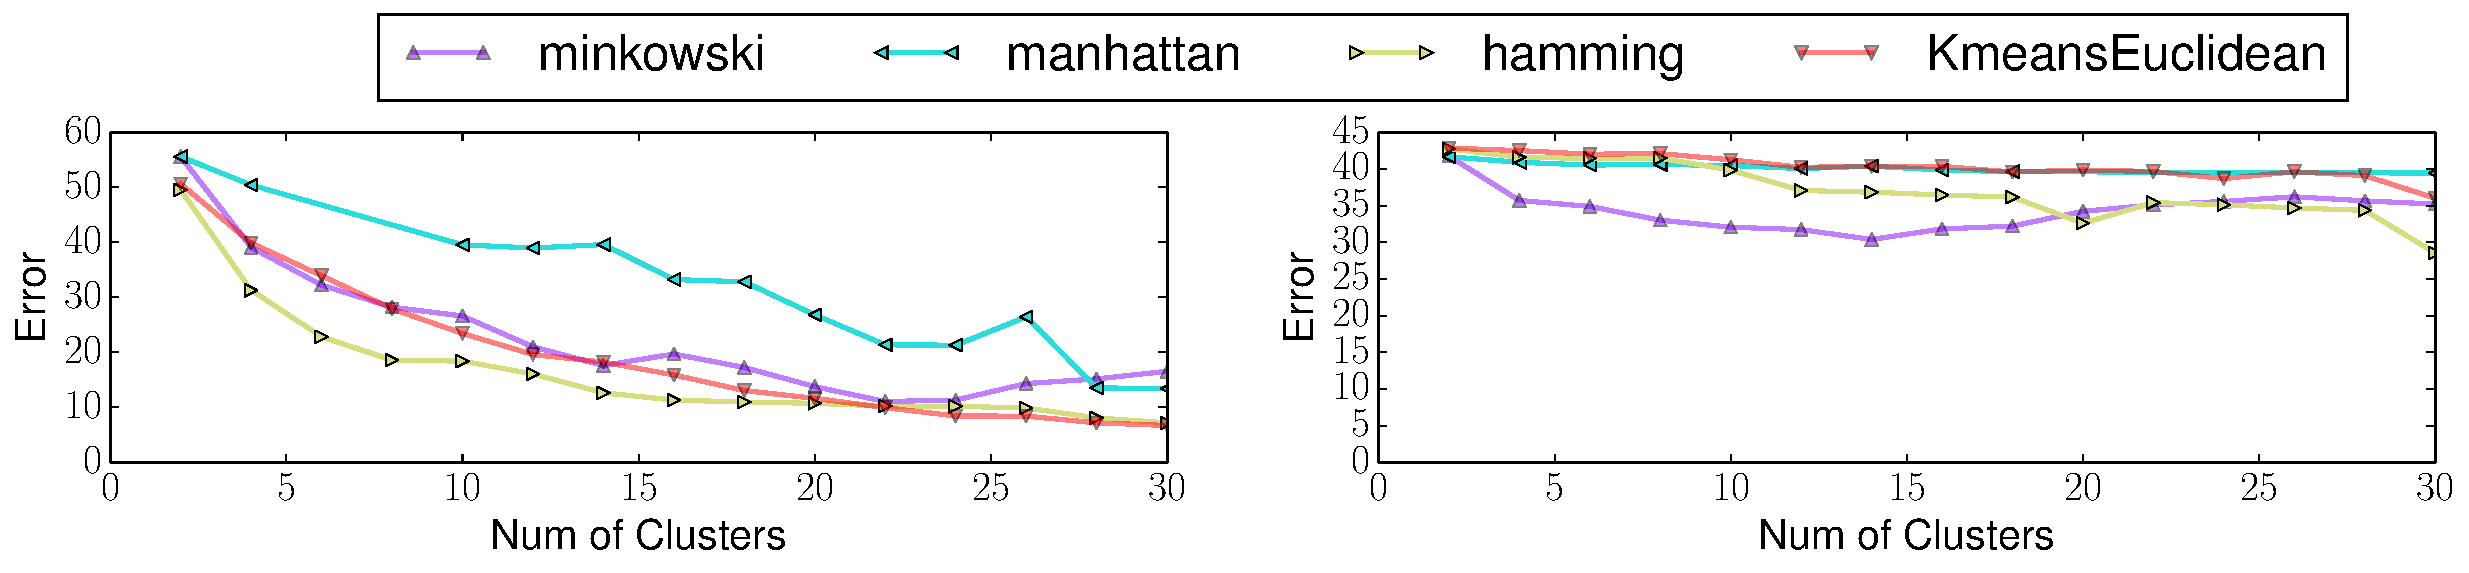
\includegraphics[width=1\textwidth]{QueryLogSummarization/graphics/ErrorVNumCluster.pdf}
 \bfcaption{Error v. Number of Clusters (Left: PocketData, Right: US Bank)}   
 \label{fig:ErrorVNumCluster}
\end{subfigure}
~
%\begin{subfigure}[b]{1\textwidth}
%    \centering      
%    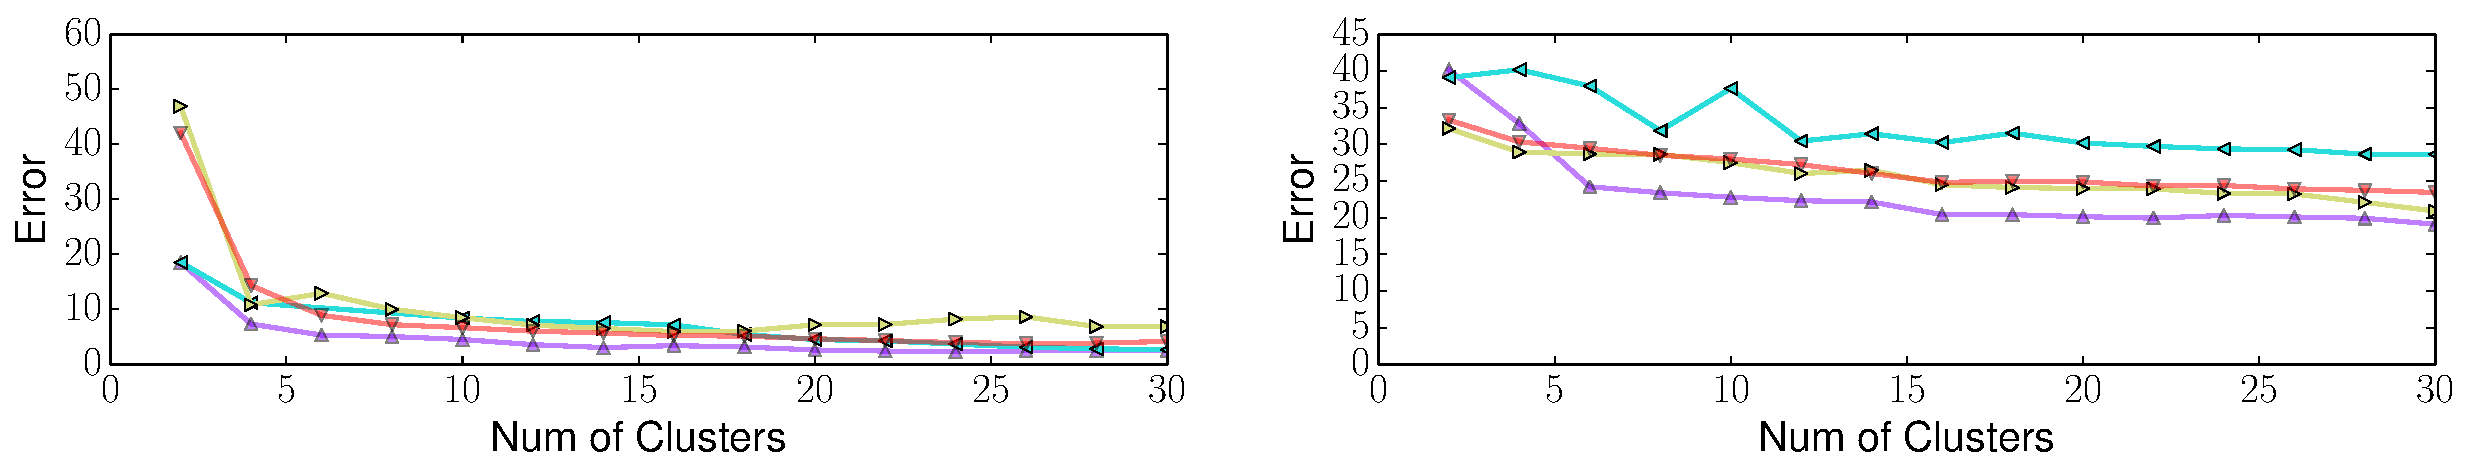
\includegraphics[width=1\textwidth]{QueryLogSummarization/graphics/MultiAdjustedErrorVNumCluster.pdf}
% \bfcaption{Error v. Number of Clusters under multiplicity-aware Clustering (Left: PocketData, Right: US Bank)}   
%\label{fig:MultiAdjustedErrorVNumCluster}
%\end{subfigure}
%~
\begin{subfigure}[b]{0.98\textwidth}
    \centering      
    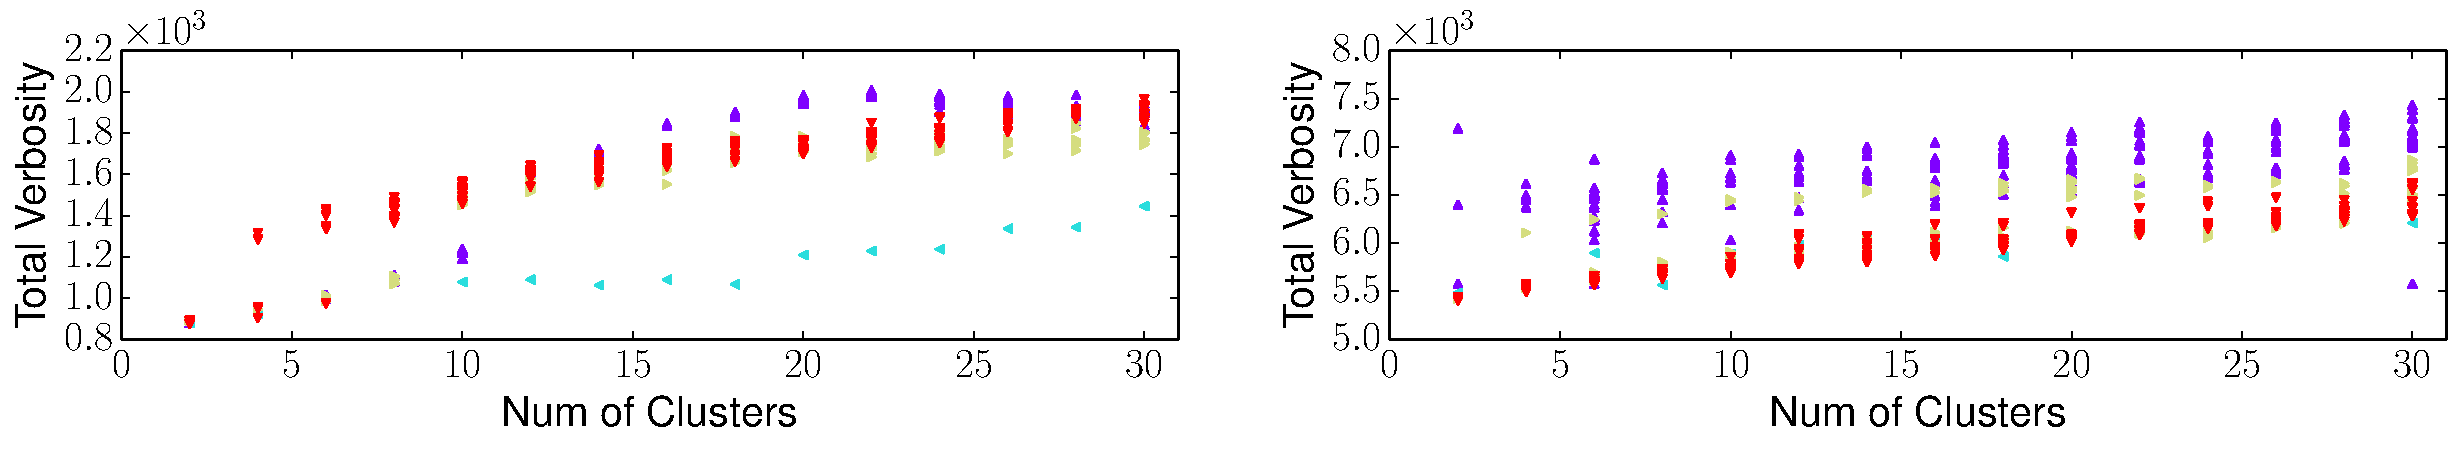
\includegraphics[width=1\textwidth]{QueryLogSummarization/graphics/TotalVerbosityVNumCluster.pdf}
 \bfcaption{Total Verbosity v. Number of Clusters (Left: PocketData, Right: US Bank); 
Each point is the verbosity of one of ten trials.  The Y-axis' lower bound is the verbosity at 1 cluster to better show the change in verbosity.}   
 \label{fig:TotalVerbosityVNumCluster}
\end{subfigure}
~
%\begin{subfigure}[b]{0.98\textwidth}
%    \centering      \includegraphics[width=1\textwidth]{QueryLogSummarization/graphics/ErrorVExpectationOfVerbosity.pdf}
% \bfcaption{Error v. Expectation of Verbosity (Left: PocketData, Right: US Bank)}   \label{fig:ErrorVExpectationOfVerbosity}
%\end{subfigure}
%~
\begin{subfigure}[b]{0.99\textwidth}
    \centering      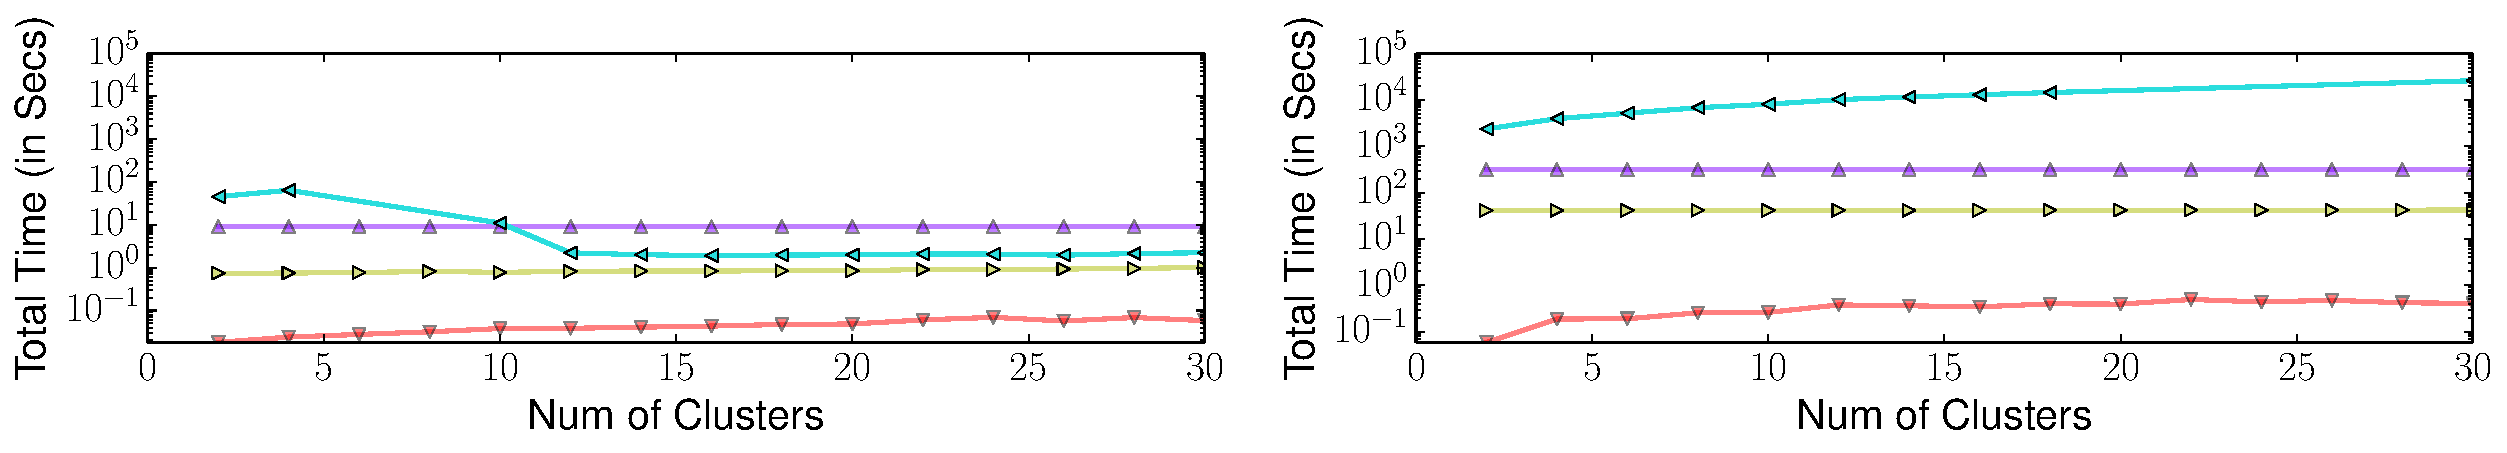
\includegraphics[width=1\textwidth]{QueryLogSummarization/graphics/RunningTimeVNumCluster.pdf}
 \bfcaption{Runtime v. Number of Clusters (Left: PocketData, Right: US Bank)}   \label{fig:RunningTimeVCluster}
\end{subfigure}
~
 \bfcaption{Clustering Schemes Comparison}
 \label{fig:distancemeasurecomparison} 
 \trimfigurewhitespace
\end{figure*}

\section{Pattern Mixture Compression}
\label{sec:constructingencodings}
We are now ready to describe the \systemnameone compression scheme.
Broadly, \systemnameone attempts to identify a pattern mixture encoding that optimizes for some target trade-off between Total Verbosity and Error.  
A naive --- though impractical --- approach to finding such an encoding would be to search the entire space of possible pattern mixture encodings.
Instead, \systemnameone approximates the same outcome by first identifying the naive mixture encoding that is closest to optimal for the desired trade-off.
As I will show experimentally, this naive mixture encoding is competitive with more complicated, slower techniques for summarizing query logs.
We also explore a hypothetical second stage, where \systemnameone refines the naive mixture encoding to further reduce Error.
The outcome of this hypothetical stage has a slightly lower Error and Verbosity, but does not admit efficient computation of database statistics. 

\subsection{Constructing Naive Mixture Encodings}
\label{sec:constructingnaivemixtureencodings}
\systemnameone searches for a naive mixture encoding that best optimizes for a requested tradeoff between Total Verbosity and Error.  
As a way to make this search efficient, we observe that a log (or log partition) uniquely determines its naive (or naive mixture) encoding. 
Thus the problem of searching for a naive mixture encoding reduces to searching for the corresponding log partitioning.
We further observe that the Error of a naive mixture encoding is proportional to the diversity of the queries in the log being encoded: 
The more uniform the log (or partition), the lower the Error.
Hence, the partitioning problem further reduces to clustering queries in the log by feature overlap.
 \begin{example}
 \label{example:twolevelnaivemixtureencoding}
 Figure~\ref{fig:hierarchicalnaivemixtureencoding} shows an example of constructing a naive mixture encoding from partitioning one cluster into two.
 The naive encodings on the child level (Figure~\ref{fig:childlevel}), each with lower Average Verbosity and Encoding Error, provide a cleaner view of the mixed workload.
 % The Average Verbosity of the resulting naive mixture encoding is lower, as is the generalized Encoding Error.
 However, note that feature \cqword{FROM}{Messages} appears in both children, so the Total Verbosity of the child level is one higher than the parent --- observers see the same feature twice.
 \end{example}
To identify a suitable clustering scheme, we next evaluate four commonly used clustering schemes with respect to their ability to create naive mixture encodings with low Error and Verbosity: (1) KMeans~\cite{DBLP:journals/prl/Jain10} with Euclidean distance (i.e., $l_2$-norm) and Spectral Clustering~\cite{DBLP:journals/jacm/KannanVV04} with (2) Manhattan (i.e., $l_1$-norm), (3) Minkowski (i.e., $l_p$-norm) with $p=4$, and (4) Hamming distances\footnote{Spectral Clustering with Euclidean, Chebyshev and Canberra distances are also evaluated; These did not perform better and I omit them in the interest of conciseness.}.
 \begin{figure}
  \centering
 \begin{subfigure}{\columnwidth}
   {\small
     \begin{tabular}{r|p{60mm}}
     \textbf{SELECT} & 
         \texttt{sms\_type},
         \textcolor{light-gray}{\texttt{external\_ids}},
         \texttt{\_time},
         \texttt{\_id}\\ \hline
     \textbf{FROM} &
         \texttt{Messages}\\ \hline
     \textbf{WHERE} &
         \texttt{(sms\_type=1)} $\wedge$
         \textcolor{mid-gray}{\texttt{(sms\_type=0)}} $\wedge$
         \texttt{(status=1)}   
         $\wedge$~\textcolor{light-gray}{\texttt{(\_time$\geq$14260)}} $\wedge$~\texttt{(transport=3)} 
     \end{tabular}
   }
   \bfcaption{\textit{Parent Level}: Naive encoding of a mixture of two workloads.}
   \label{fig:parentlevel}
 \end{subfigure}\\[2mm]
 \begin{subfigure}{\columnwidth}
 \hspace*{-1mm}
   {\small
     \centering
     \begin{tabular}{r|p{20mm}}
     \textbf{SELECT} & 
         \texttt{sms\_type},\texttt{\_time}
         \\ \hline
     \textbf{FROM} &
         \texttt{Messages}\\ \hline
     \textbf{WHERE} &
         \texttt{(sms\_type=1)}$\wedge$ 
         \textcolor{mid-gray}{\texttt{(sms\_type=0)}}$\wedge$
         \textcolor{light-gray}{\texttt{(\_time$\geq$14260)}}  
     \end{tabular}
     \begin{tabular}{r|p{20mm}}
     \textbf{SELECT} & 
         \texttt{\_id}, \textcolor{light-gray}{\texttt{external\_ids}}
         \\ \hline
     \textbf{FROM} &
         \texttt{Messages}\\ \hline
     \textbf{WHERE} &
         \texttt{(status=1)}$\wedge$
         \texttt{(transport=3)} 
     \end{tabular}
   }
   \bfcaption{\textit{Child Level}: Two children encodings that separately summarize each workload.}
   \label{fig:childlevel}  
 \end{subfigure}\\[2mm]
 \bfcaption{\textbf{Constructing a naive mixture encoding}}
 \label{fig:hierarchicalnaivemixtureencoding}
 \trimfigurewhitespace
 \end{figure}

\tinysection{Experiment Setup}
Spectral and KMeans clustering algorithms are implemented by \textit{sklearn}~\cite{scikit-learn} in Python. 
We gradually increase $K$ (i.e., the number of clusters) for each clustering scheme to mimic the process of continuously sub-clustering the log, tolerating higher Total Verbosity for lower Error.
To reduce randomness in clustering, we run each of them $10$ times for each $K$ and averaging the Error of the resulting encodings.  
We use two datasets: ``US Bank'' and ``PocketData''.  
Both datsets and the data preparation process are described in detail in Section~\ref{sec:commonexperimentsettings}. 
All results for our clustering experiments are shown in Figure~\ref{fig:distancemeasurecomparison}.

\subsubsection{Clustering}
\label{sec:clustering}
I next show that clustering is an effective way to consistently reduce Error, although no one clustering scheme is ideal for all three of Error, Verbosity, and runtime.

\tinysection{More clusters reduces Error}
Figure~\ref{fig:ErrorVNumCluster} compares the relationship between the number of clusters (x-axis) and Error (y-axis), showing the varying rates of convergence to zero Error for each clustering scheme.
We observe that adding more clusters does consistently reduce Error for both data sets, regardless of clustering algorithm or distance measure.
We note that the US Bank dataset is significantly more diverse than the PocketData dataset, with respect to the total number of features (See Table~\ref{table:datasummary}) and that more than $30$ clusters may be required for reaching near-zero Error.
In general, Hamming distance converges faster than other distance measures on PocketData.
Minkowski distance shows faster convergence rate than Hamming within $14$ clusters on the US bank dataset. 

\tinysection{Adding more clusters increases Verbosity}
Figure~\ref{fig:TotalVerbosityVNumCluster} compares the relationship between the number of clusters (x-axis) and Verbosity (y-axis).
We observe that Verbosity increases with the number of clusters.
This is because when a partition is split, each feature common to both partitions increases the Verbosity by one (as shown in Example~\ref{example:twolevelnaivemixtureencoding}).

\tinysection{Hierarchical Clustering}
The clustering schemes produce non-monotonic cluster assignments. That is, Error can occasionally grow as clusters are added (Figure~\ref{fig:ErrorVNumCluster}). 
An alternative is to use hierarchical clustering~\cite{DBLP:journals/prl/Jain10}, which forces monotonic assignments and offers more dynamic control over the Error/Verbosity tradeoff.

\tinysection{Run Time Comparison}
The total runtime (y-axis) in Figure~\ref{fig:RunningTimeVCluster} includes both distance matrix computation time (if any) and clustering time. 
Note the log-scale: K-Means is orders of magnitude faster than the others.

\tinysection{Take-Aways}
For time-sensitive applications, KMeans algorithm is preferred to Spectral Clustering.
With respect to distance measures, minkowski (i.e., $l_p$-norm) with $p=4$ provides the best tradeoff between Error and runtime.

\tinysection{Visualizing Naive Mixture Encoding}
As with normal pattern summaries, naive mixture summaries are also interpretable.
For example a visualization like that of Figure~\ref{fig:screenshots:nocorrelation} can be repeated, once for each cluster.  
For more details, see our accompanying technical report~\cite{DBLP:journals/corr/abs-1809-00405}.

\subsection{Approximating Log Statistics}
Recall that our primary goal is estimating frequencies.
In particular, we are interested in counting the occurrences $\Gamma_\pattern(L)$ (i.e., $p(Q\supseteq\vec b)\cdot |L|$) of some pattern $\pattern$ in the log.
%$$\Gamma_\pattern(L) = |\comprehension{\vec q}{\vec q \in L \wedge \pattern \subseteq \vec q}|$$
Recall that a naive encoding $\naiveencoding$ includes only single-feature patterns (i.e., patterns exactly encoding $p(X_i\ge x_i)$) and that the closed-form representation for the maximum entropy distribution $\overline \rho_{\naiveencoding}$ arises by independence between features (i.e., $\overline \rho_{\naiveencoding}(Q = \vec q) = \prod_{i} p(X_i = x_i)$).
Similarly, we use the independence assumption to estimate:
$$est[\Gamma_\pattern(L)\;|\;\naiveencoding]=\overline \rho_{\naiveencoding}(Q \supseteq \vec b)\cdot |L| = \prod_{i} p(X_i \geq x_i)\cdot |L|$$

This process trivially generalizes to naive pattern mixture encodings by mixing distributions.  
Specifically, given a set of partitions $L_1 \cup \ldots \cup L_K = L$, the estimated counts for $\Gamma_\pattern(L)$ under each individual partition $L_i$ can be computed based on the partition's naive encoding $\naiveencoding_i$, and we then sum up the estimated counts in each partition:
$$est[\;\Gamma_\pattern(L_i)\;|\;\naiveencoding_1, \ldots, \naiveencoding_K\;] = \sum_{i \in [1, K]} est[\;\Gamma_\pattern(L_i)\;|\;\naiveencoding_i\;]$$

\begin{figure*}[h!]
\captionsetup[subfigure]{justification=centering}
    \centering 
    
\begin{subfigure}[b]{0.48\textwidth}
    \centering     
     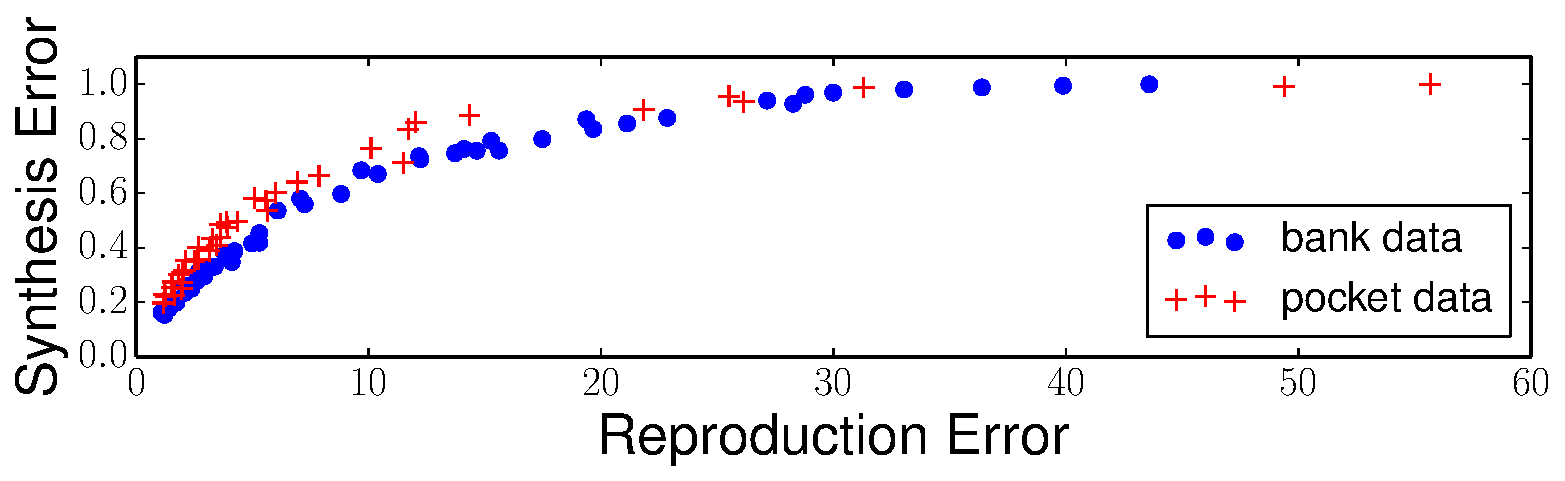
\includegraphics[width=1\textwidth]{QueryLogSummarization/graphics/synthesis_error.pdf}
 \bfcaption{Synthesis Error v. \Errorname}   
 \label{fig:synthesis_error_versus_reproduction_error}
\end{subfigure}
~
\begin{subfigure}[b]{0.48\textwidth}
    \centering      
    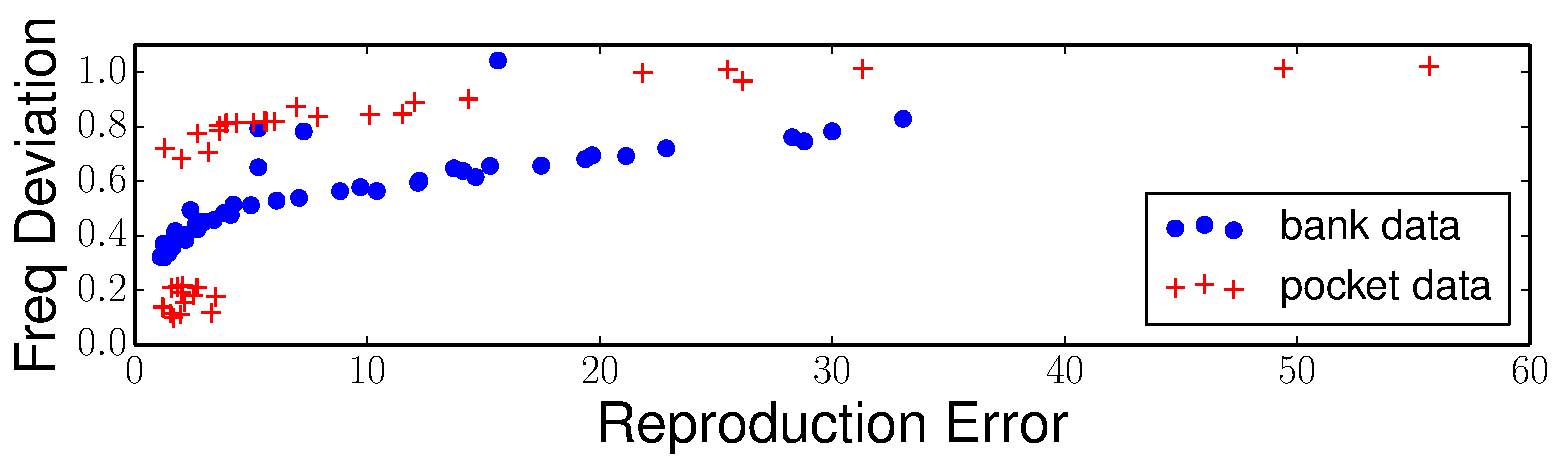
\includegraphics[width=1\textwidth]{QueryLogSummarization/graphics/marginal_deviation.pdf}
 \bfcaption{Frequency Deviation v. \Errorname}   
 \label{fig:marginal_deviation_versus_reproduction_error}
\end{subfigure}

 \bfcaption{Effectiveness of Naive Mixture Encoding}
 \label{fig:effectiveness_of_naive_mixture_encoding} 
 \trimfigurewhitespace
\end{figure*} 

\subsection{Pattern Synthesis \& Frequency Estimate}
In this section, we empirically verify the effectiveness of naive mixture encodings in approximating log statistics from two related perspectives. 
The first perspective focuses on \textit{synthesis error}. 
It measures whether patterns synthesized by the naive mixture encoding actually appear in the log.
From the second perspective, we further investigate the \textit{frequency deviation} of patterns contained in the log.
This evaluates whether a naive mixture encoding computes the correct frequency for patterns of interest to client applications.
Experimental results are shown in Figure~\ref{fig:effectiveness_of_naive_mixture_encoding}.
Both synthesis error and frequency deviation consistently decrease given more clusters.
Furthermore, as we vary the number of clusters, both measures correlate with \errorname.

\noindent \textbf{Synthesis Error}
is measured by $1-\frac{m}{n}$ where $m$ out of $n$ randomly synthesized patterns actually appear in the log.
Intuitively, when synthesis error grows, it is more likely that a pattern from the synthesized log will not appear in the original log (i.e., smaller values are better).
Figure~\ref{fig:synthesis_error_versus_reproduction_error} shows synthesis error (y-axis) versus \errorname (x-axis).
The figure is generated by synthesizing $n=10000$ patterns from each cluster of the log.
Note that different values of $n$ give similar observations.
The overall synthesis error is measured by the average of synthesis errors for all clusters, weighted by the proportion of queries in each cluster.

\noindent \textbf{Frequency Deviation}
is measured for a pattern by $\frac{|est-t|}{t}$ where $t$ stands for true frequency of a pattern and $est$ is the one estimated by the naive mixture encoding.
Since frequency deviation is smaller when evaluated on a pattern contained in the other, as an alternative, we treat each distinct query in the log as a pattern and the frequency deviation on it will be the worst case for all patterns that it contains.
Intuitively, this value captures the percentage error of frequency estimates (i.e., smaller values are better).
For each cluster, we sum frequency deviations on all of its distinct queries and the final frequency deviation for the whole log is an weighted average (same as synthesis error) over all clusters.
Figure~\ref{fig:marginal_deviation_versus_reproduction_error} shows frequency deviation (y-axis) versus \errorname (x-axis).

\subsection{Naive Encoding Refinement}
\label{sec:naivemixtureencodingrefinement}
Naive mixture encodings can already achieve close to near-zero Error (Figure~\ref{fig:ErrorVNumCluster}), have low Total Verbosity, and admit efficiently computable log statistics $\Gamma_\pattern(L)$.
Doing so makes estimating statistics more computationally expensive.
However, as a thought experiment we consider a hypothetical second pass to enrich naive mixture encodings with non-naive patterns.
We start by considering the simpler problem of identifying the \emph{individual} non-naive pattern that maximally reduces the \errorname of a naive encoding.

\tinysection{Feature-Correlation Refinement}
Recall that under naive encodings, we have a closed-form estimation $\overline \rho_{\naiveencoding}(Q \supseteq \vec b)$ of pattern frequencies $p(Q\supseteq\vec b)$.
We thus define the \textit{feature-correlation} of pattern $\vec b$ as the log-difference from its actual frequency to the estimate.
$$fc(\vec b, \naiveencoding) = |\log\left(
    p(Q \supseteq \vec b)
\right) - \log\left(
  %\prod_{i} p(X_i \geq x_i)
  \overline \rho_{\naiveencoding}(Q \supseteq \vec b)
\right)|$$
Intuitively, patterns with higher feature correlations carry more information content of the log that its naive encoding ignores, making them ideal candidates for addition to the naive encoding.
For two patterns with the same feature-correlation, the one that occurs more frequently~\cite{DBLP:journals/datamine/HanCXY07} will have greater impact on \errorname. 
As a result, we compute an overall score for ranking individual patterns:  
$$corr\_rank(\vec{b})=p(Q \supseteq \vec b) \cdot fc(\vec b, \naiveencoding)$$
I will show in Section~\ref{sec:motivateencodingerror} that $corr\_rank$ closely correlates with \errorname.
That is, a higher $corr\_rank$ value indicates that a pattern produces a greater reduction in \errorname if introduced into the naive encoding.

\tinysection{Pattern Diversification}
In general, we would like to identify a \emph{set} of patterns.
The greedy approach that adds patterns one by one based on their ranking scores $corr\_rank$ is unreliable, as modifying the naive encoding invalidates the closed-form estimation $\overline \rho_{\naiveencoding}(Q \supseteq \vec b)$ that score $corr\_rank$ relies on.
In other words, we can not sum up $corr\_rank$ scores of patterns in a set in order to rank its overall contribution to \errorname reduction, as information content carried by patterns may overlap.
To counter such overlap, or equivalently to \textit{diversify} patterns, a search through the space of pattern-sets is needed.
This type of diversification is commonly used in pattern mining applications, but can quickly become expensive.
As I show experimentally in Section~\ref{sec:motivatepatternmixturesummaries}, the benefit of diversification is minimal.





\section{Experiments}
\label{sec:experiments}
In this section, we design experiments to empirically (1) validate that \errorname correlates with Deviation and (2)~evaluate the effectiveness of \systemnameone compression.

We use two specific datasets in the experiment: (1) SQL query logs of the Google+ Android app extracted from the PocketData public dataset~\cite{DBLP:conf/tpctc/KennedyACZ15} and (2) SQL query logs that capture all query activity on the majority of databases at a major US bank over a period of approximately 19 hours.
A summary of these two datasets is given in Table~\ref{table:datasummary}.

\begin{table}
\centering
\bfcaption{Summary of Data sets}
\label{table:datasummary}
{\small \centering
\begin{tabular}{c c c}
\toprule
Statistics & PocketData & US bank \\
\midrule
\# Queries & 629582& 1244243\\
\midrule
\# Distinct queries & 605& 188184\\
\midrule
\# Distinct queries (w/o const)& 605& 1712\\
\midrule
\# Distinct conjunctive queries & 135& 1494\\
\midrule
\# Distinct re-writable queries & 605& 1712\\
\midrule
Max query multiplicity & 48651 & 208742\\
\midrule
\# Distinct features & 863& 144708\\
\midrule
\# Distinct features (w/o const) & 863& 5290\\
\midrule
Average features per query & 14.78& 16.56\\
\bottomrule
\end{tabular}
}
\trimfigurewhitespace
\end{table}

\begin{figure*}[h!]
	\captionsetup[subfigure]{justification=centering}
    \centering
    \begin{subfigure}[b]{0.48\textwidth}
        \centering
        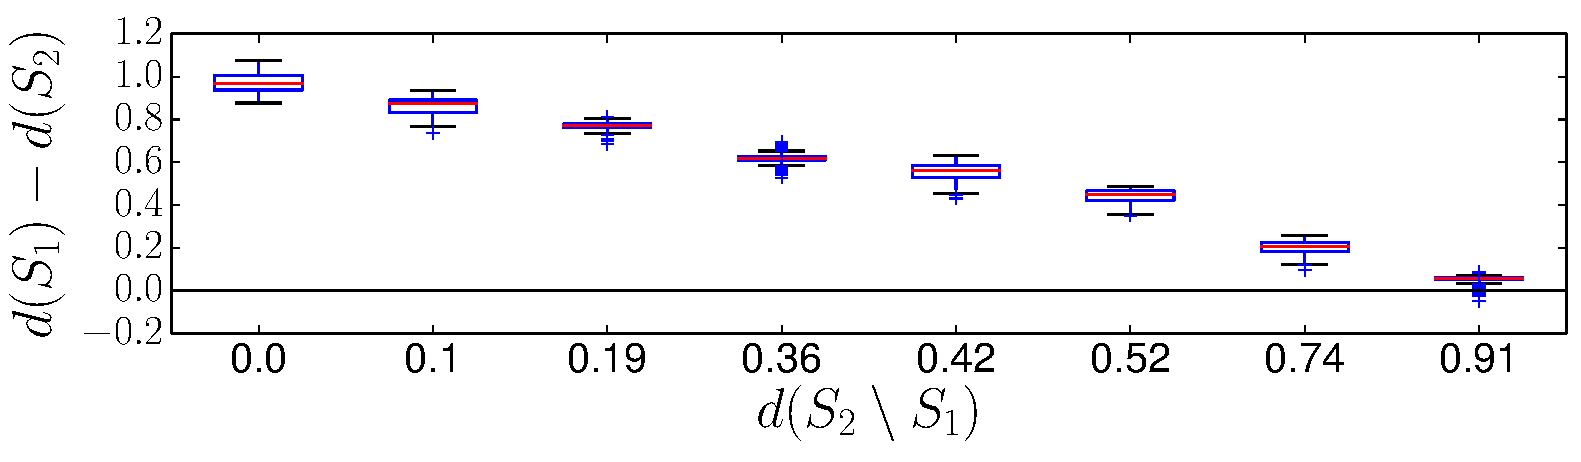
\includegraphics[width=\textwidth]{QueryLogSummarization/graphics/ContainmentCapturesDeviation_BankData.pdf}
        \bfcaption{Containment captures Deviation (US bank)}
        \label{fig:containmentcapturesdeviation_bankdata}
    \end{subfigure}
        ~
    \begin{subfigure}[b]{0.48\textwidth}
        \centering
        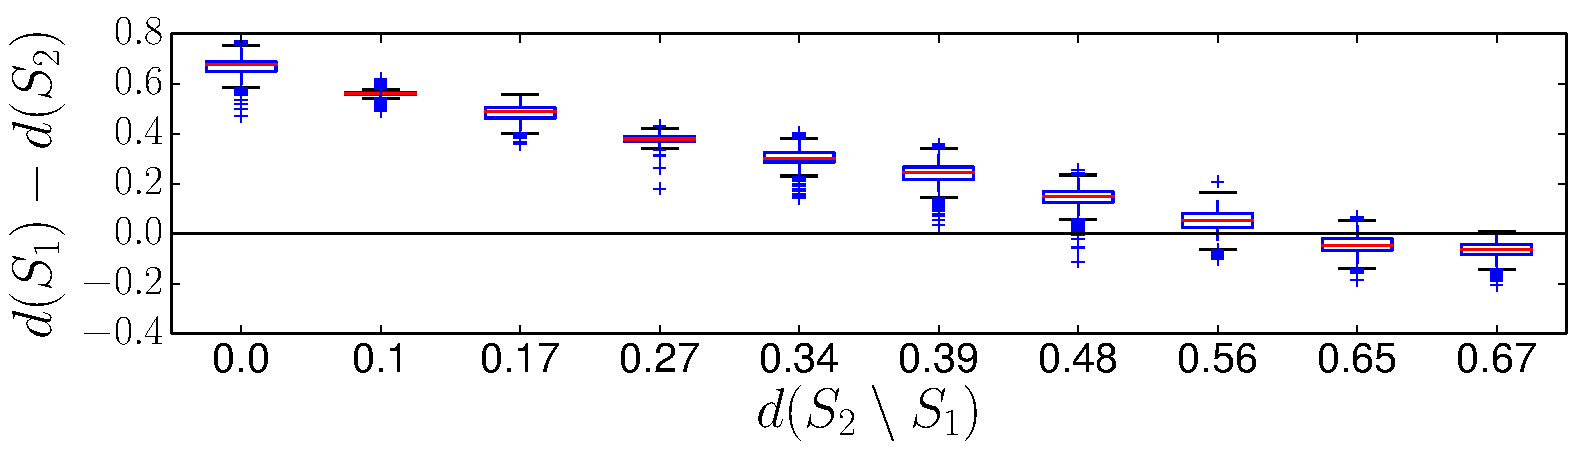
\includegraphics[width=\textwidth]{QueryLogSummarization/graphics/ContainmentCapturesDeviation_PocketData.pdf}
        \bfcaption{Containment captures Deviation (PocketData)}
        \label{fig:containmentcapturesdeviation_pocketdata}
    \end{subfigure}
    ~
    \begin{subfigure}[b]{0.485\textwidth}
        \centering
         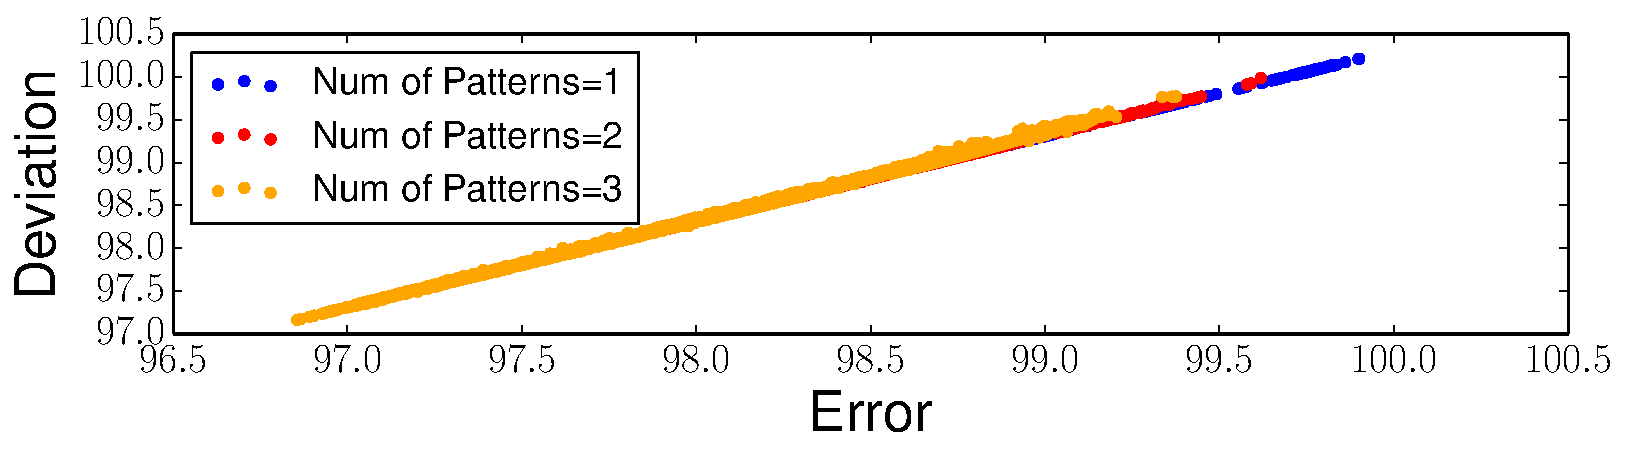
\includegraphics[width=\textwidth]{QueryLogSummarization/graphics/ErrorCapturesDeviation_BankData.pdf}
        \bfcaption{Error captures Deviation (US bank)}
        \label{fig:errorcapturesdeviation_bankdata}
    \end{subfigure}
        ~
    \begin{subfigure}[b]{0.485\textwidth}
        \centering
        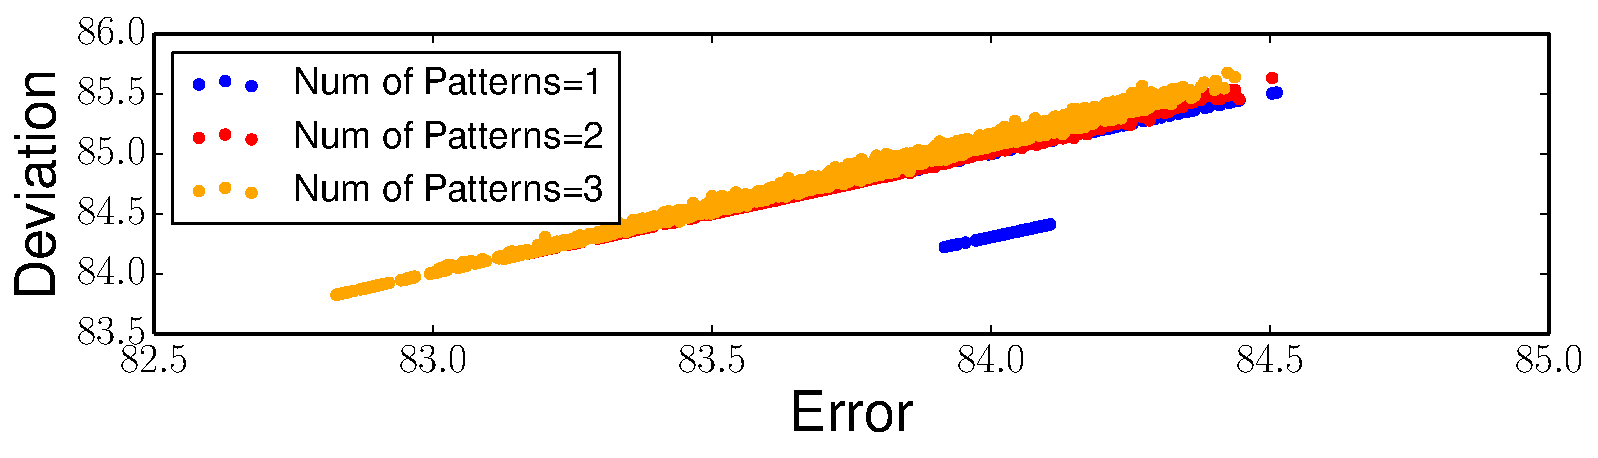
\includegraphics[width=\textwidth]{QueryLogSummarization/graphics/ErrorCapturesDeviation_PocketData.pdf}
        \bfcaption{Error captures Deviation (PocketData)}
        \label{fig:errorcapturesdeviation_pocketdata}
    \end{subfigure}
    ~
     \begin{subfigure}[b]{0.45\textwidth}
        \centering
        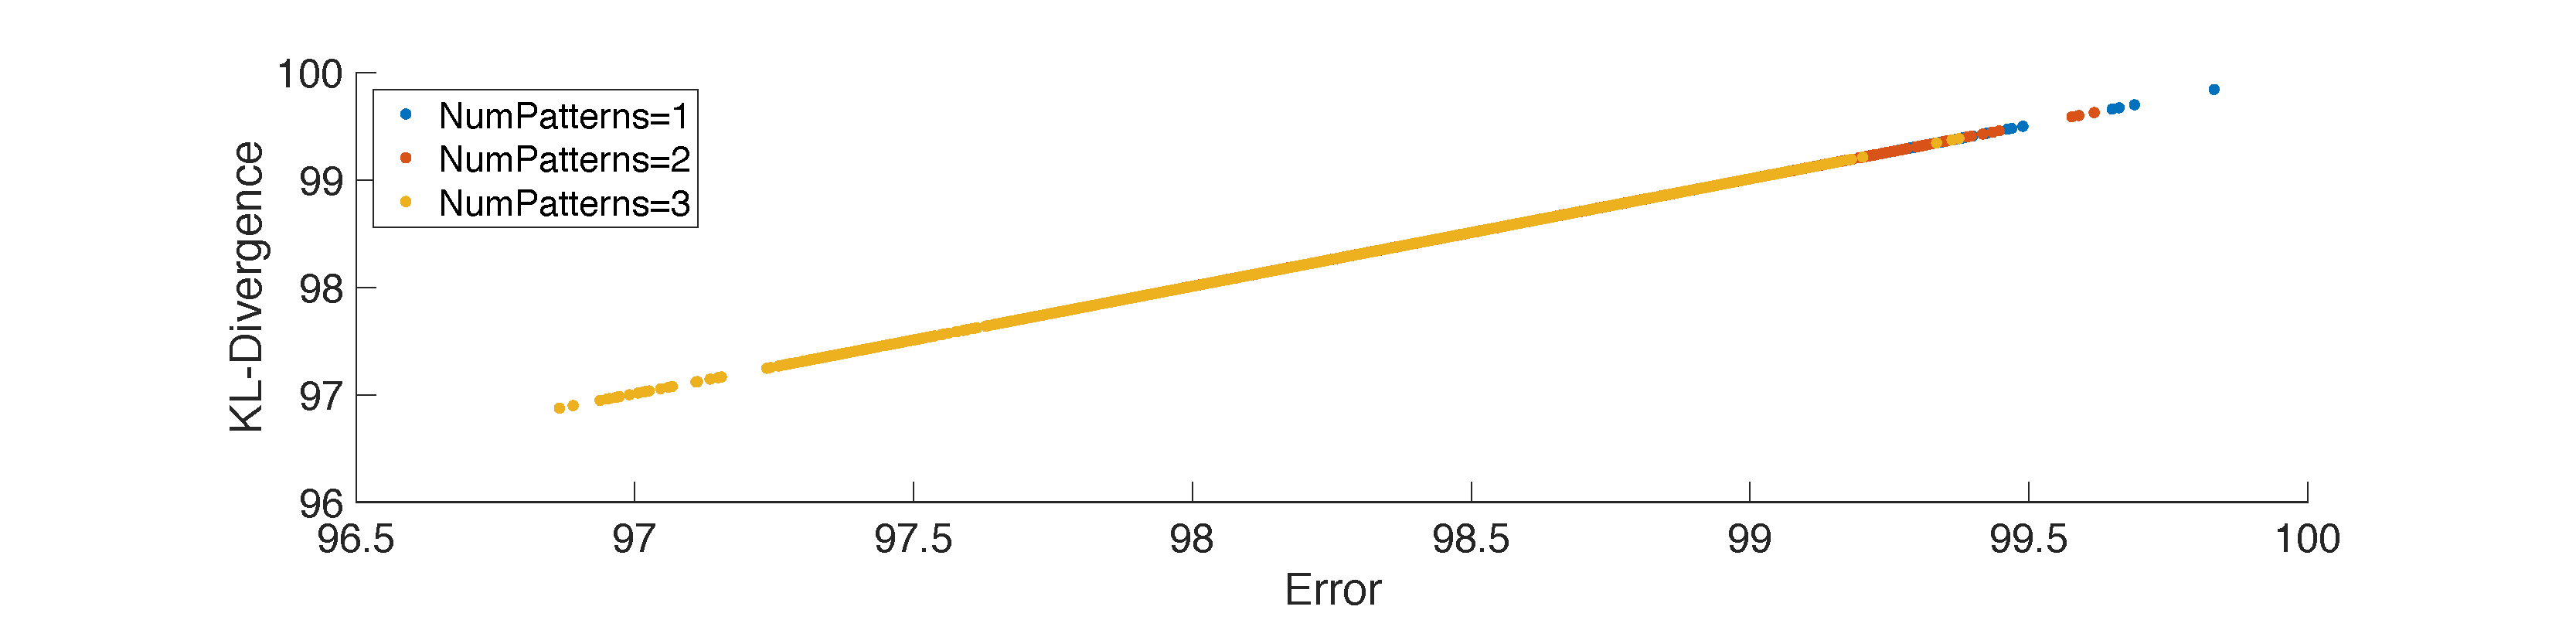
\includegraphics[width=\textwidth]{QueryLogSummarization/graphics/ErrorCapturesKL_BankData.pdf}
        \bfcaption{Error captures KL-divergence (US bank)}
        \label{fig:errorcapturesKL_bankdata}
\end{subfigure}
    ~
     \begin{subfigure}[b]{0.45\textwidth}
        \centering
        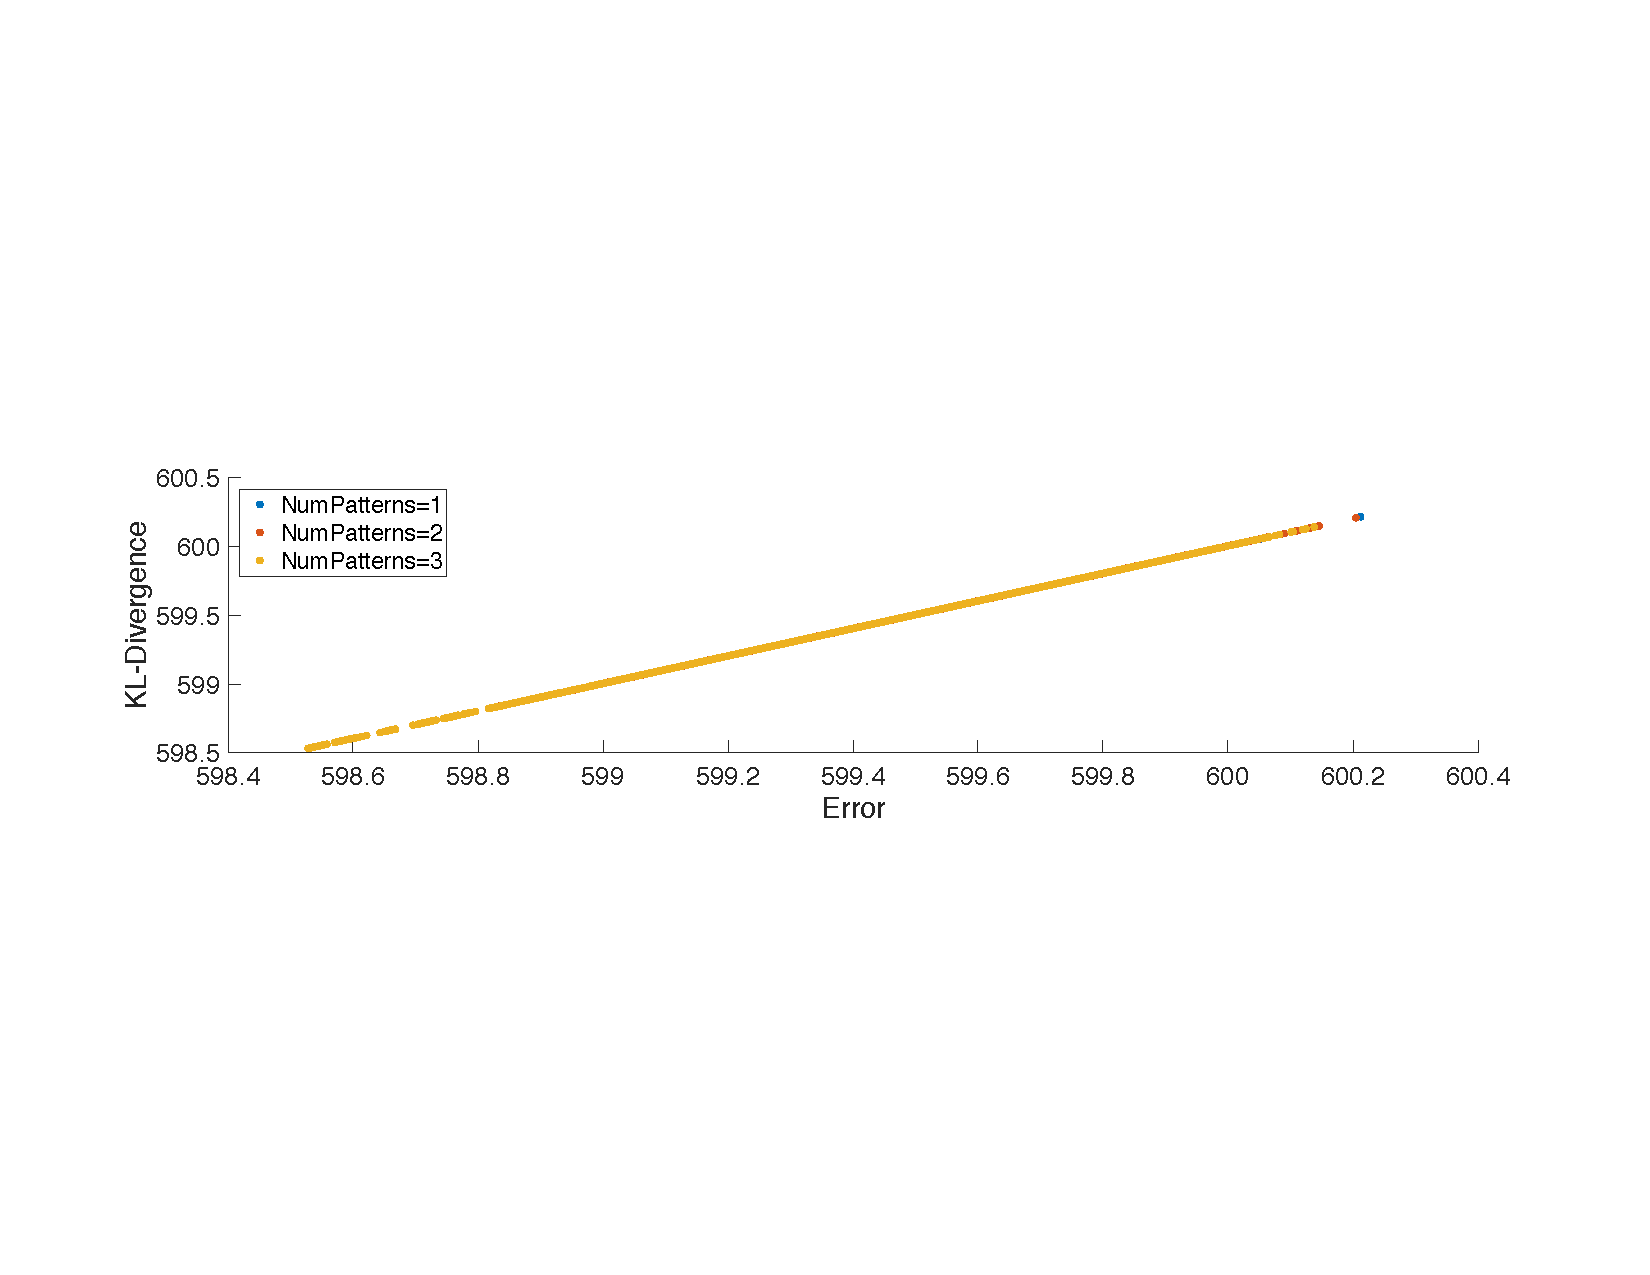
\includegraphics[width=\textwidth]{QueryLogSummarization/graphics/ErrorCapturesKL_PocketData.pdf}
        \bfcaption{Error captures KL-divergence (PocketData)}
        \label{fig:errorcapturesKL_pocketdata}
\end{subfigure}
    ~
     \begin{subfigure}[b]{0.48\textwidth}
        \centering     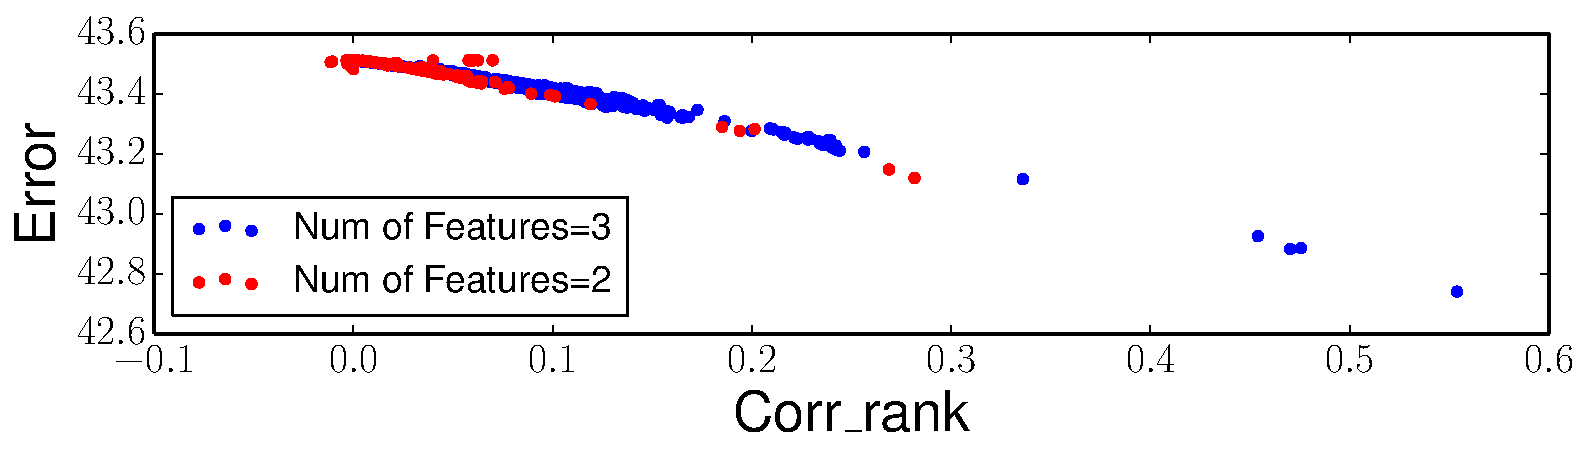
\includegraphics[width=\textwidth]{QueryLogSummarization/graphics/ErrorCapturesCorrelation_BankData.pdf}
        \bfcaption{Error captures Correlation (US bank)}
        \label{fig:errorcapturescorrelation_bankdata}
\end{subfigure}
    ~
     \begin{subfigure}[b]{0.48\textwidth}
        \centering     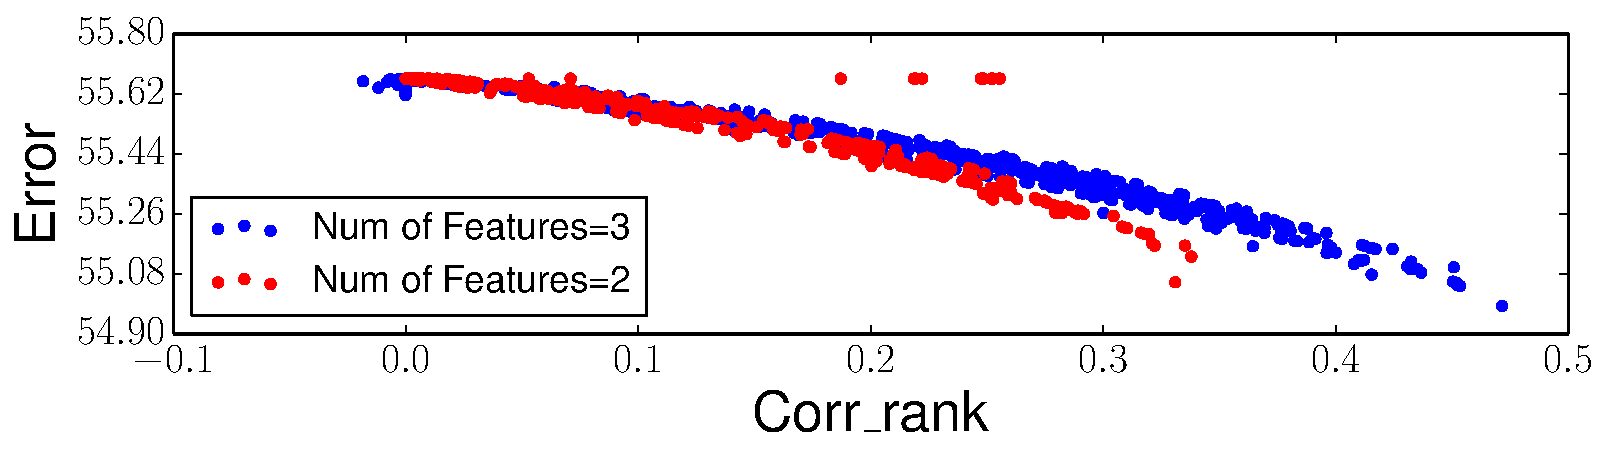
\includegraphics[width=\textwidth]{QueryLogSummarization/graphics/ErrorCapturesCorrelation_PocketData.pdf}
        \bfcaption{Error captures Correlation (PocketData)}
        \label{fig:errorcapturescorrelation_pocketdata}
\end{subfigure}
    
\bfcaption{Validating \Errorname}
\label{fig:validatingencodingerror}
\trimfigurewhitespace
\end{figure*}

\tinysection{The PocketData-Google+ query log} 
The dataset consists of SQL logs that capture all database activities of 11 Android phones. 
I selected the Google+ application for our study since it is one of the few applications where all users created a workload. 
This dataset is a stable workload of exclusively machine-generated queries.

\tinysection{The US bank query log}
This log is an anonymized record of queries processed by multiple relational database servers at a major US bank~\cite{DBLP:conf/www/KulLXCCKU16} over a period of 19 hours.
Of the nearly 73 million database operations captured, 58 million are not directly queries, but rather invocations of stored procedures.
A further 13 million used non-standard SQL features not supported by our SQL parser. 
Of the remaining of the 2.3 million parsed SQL queries, I base the analysis on the 1.25 million conjunctive \texttt{SELECT} queries. 
This dataset can be characterized as a diverse workload of both machine- and human-generated queries.

\tinysection{Common Experiment Settings}
\label{sec:commonexperimentsettings}
Experiments were performed on a 2.8 GHz Intel Core i7 CPU with 16 GB 1600 MHz DDR3 memory and a SSD running macOS Sierra.

\tinysection{Constant Removal}
A number of queries in the US bank query log differ only in hard-coded constant values.
Table~\ref{table:datasummary} shows the total number of queries, as well as the number of distinct queries if we ignore constants.
By comparison, queries in PocketData all use JDBC parameters.
For these experiments, we ignore constant values in queries.

\tinysection{Query Regularization}
We apply query rewrite rules (same as \cite{8352666}) to regularize queries into equivalent conjunctive forms, where possible. 
Table~\ref{table:datasummary} shows that $\frac{135}{605}$ and $\frac{1494}{1712}$ of distinct queries are in conjunctive form for PocketData and US bank respectively. 
After regularization, all queries in both data sets can be either simplified into conjunctive queries or re-written into a \texttt{UNION} of conjunctive queries compatible with feature scheme of Aligon et al.~\cite{DBLP:journals/kais/AligonGMRT14}.

\tinysection{Convex Optimization Solving}
All convex optimization problems for measuring \errorname and Deviation are solved by the \textit{successive approximation heuristic} implemented by the CVX toolbox~\cite{cvx} with the Sedumi solver.

\subsection{Validating \Errorname}
\label{sec:motivateencodingerror}
In this section, we validate that \errorname is a practical alternative to Deviation.
In addition, I also offer measurements on its correlation with Deviation and score $corr\_rank$ in Section~\ref{sec:naivemixtureencodingrefinement}.
%
As it is impractical to enumerate all possible encodings, I choose a subset of encodings for both datasets. 
Specifically, I first select all features with frequencies in the range $[0.01,0.99]$ and use these features to construct patterns.
I then enumerate combinations of $K$ (up to 3) patterns as our chosen encodings.

\tinysection{Containment Captures Deviation}
Here we empirically verify that containment (Section~\ref{sec:validateencodingerror}) captures Deviation (i.e., $\encoding_1\leq_{\Omega} \encoding_2\to d(\encoding_1)\leq d(\encoding_2)$) to complete the chain of reasoning that \errorname captures Deviation.
Figures~\ref{fig:containmentcapturesdeviation_bankdata} and \ref{fig:containmentcapturesdeviation_pocketdata} show all pairs of encodings where $\encoding_2\supset \encoding_1$.
The y-axis shows the difference in Deviation values (i.e., $d(\encoding_2)-d(\encoding_1)$).
Deviation $d(\encoding)$ is approximated by drawing 1 million samples from the space $\Omega_{\encoding}$ induced by the encoding $\encoding$.
For clarity, I bin pairs of encodings by the degree of overlap between them, measured by the Deviation of the set-difference $d(\encoding_2\setminus \encoding_1)$; Higher $d(\encoding_2\setminus \encoding_1)$ implies less overlap. 
Y-axis values are grouped into bins and visualized by boxplot where the boxes represent ranges within standard deviation and crosses are outliers.
Intuitively, \emph{points above zero} on the y-axis (i.e., $d(\encoding_2)-d(\encoding_1) > 0$) are pairs of encodings where the Deviation order agrees with containment order.
This is the case for virtually all encoding pairs.  

\tinysection{Additive Separability of Deviation}
We also observe from Figures~\ref{fig:containmentcapturesdeviation_bankdata} and ~\ref{fig:containmentcapturesdeviation_pocketdata} that agreement between Deviation and containment order is correlated with overlap: More similar encodings are more likely to have agreement.
Combined with Proposition~\ref{prop:monotone}, this shows first that for similar encodings, \errorname is likely to be a reliable indicator of Deviation.
This also suggests that Deviation is additively separable: The information loss (i.e., $d(\encoding_2)-d(\encoding_1)$) caused by excluding the encoding $\encoding_2\setminus \encoding_1$ from $\encoding_2$ correlates with the quality (i.e., $d(\encoding_2\setminus \encoding_1)$) of the encoding $\encoding_2\setminus \encoding_1$ itself:\vspace*{-4mm}

{\small
$$\encoding_2\supset \encoding_1\to d(\encoding_2)-d(\encoding_1)<0\hspace{5mm}\text{and}\hspace{5mm}d(\encoding_2\setminus \encoding_1)\propto d(\encoding_2)-d(\encoding_1)$$ 
}\vspace*{-5mm}

\tinysection{Error correlates with Deviation}
As a supplement, Figures~\ref{fig:errorcapturesdeviation_bankdata} and ~\ref{fig:errorcapturesdeviation_pocketdata} empirically confirm that that \errorname (x-axis) indeed closely correlates with Deviation (y-axis).
Mirroring our findings above, correlation between them is tighter at lower \errorname.

\tinysection{Error Correlates With KL-Divergence}
Figures~\ref{fig:errorcapturesKL_bankdata} and ~\ref{fig:errorcapturesKL_pocketdata} show the relationship between \errorname (x-axis) and KL-Divergence between the true distribution $\rho^*$ and the space representative distribution $\overline{\rho}_S$ (y-axis), as discussed in Section~\ref{sec:maximumentropydistribution}. The two are tightly correlated.

\tinysection{Error and Feature-Correlation}
Figure~\ref{fig:errorcapturescorrelation_bankdata} and ~\ref{fig:errorcapturescorrelation_pocketdata} show the relationship between \errorname (y-axis) and score $corr\_rank$ (x-axis), as discussed in Section~\ref{sec:naivemixtureencodingrefinement}. Values of y-axis are \errorname of the naive encodings extended by a non-naive pattern $\vec{b}$ containing multiple features (up to 3 for illustrative purposes). 
One can observe that \errorname of extended naive encodings almost linearly correlates with $corr\_rank(\vec b)$. 
In addition, one can also observe that $corr\_rank$ becomes higher when the pattern $\vec{b}$ encodes more correlated features. 

\subsection{Feature-Correlation Refinement}
\label{sec:motivatepatternmixturesummaries}
In this section, I design experiments serving two purposes: (1) Evaluating the potential reduction of Error from refining naive mixture encodings through state-of-the-art pattern-based summarizers, and (2) Evaluating whether we can replace naive mixture encodings by the encodings created from summarizers that we have plugged-in.

\hyphenation{Laser-light}

\tinysection{Experiment Setup}
To serve both purposes, we construct pattern mixture encodings under three configurations: (1)~Naive mixture encodings; (2)~Pattern-based encodings and (3)~Naive mixture encodings refined into pattern-based encodings.
Naive mixture encodings are constructed by K-Means clustering. 
Pattern-based encodings are generated by two state-of-the-art pattern-based summarizers: 
(1)~\textit{Laserlight}~\cite{DBLP:journals/pvldb/GebalyAGKS14} that summarizes multi-dimensional data in order to predict an augmented binary variable and 
(2)~\textit{MTV}~\cite{DBLP:journals/tkdd/MampaeyVT12} that aims at mining maximally informative patterns that summarize binary multi-dimensional data. 
Detailed descriptions and experiment configurations of these two algorithms are given in Appendix~\ref{appendix:experimentsettingsforpatternbasedalgorithms}.

The experimental results are shown in Figure~\ref{fig:motivatenaivemixtureencodings_bankdata} that contains 3 sub-figures sharing the same x-axis, i.e., the number of clusters.
Figure~\ref{fig:PatternMixtureEncodingErrorComparisonAlone_bankdata} compares the Error (y-axis) between naive mixture encodings and pattern mixture encodings that consist of patterns mined from \textit{MTV} or \textit{Laserlight}.
Figure~\ref{fig:PatternMixtureEncodingErrorComparisonPiggybacking_bankdata} evaluates the change in Error (y-axis) through refining naive mixture encodings by adding patterns from \textit{MTV} or \textit{Laserlight}.
Figure~\ref{fig:mixtureencodingsrunningtimecomparison_bankdata} compares the runtime (y-axis) between constructing naive mixture encodings and applying \textit{MTV} or \textit{Laserlight}.
I only show the results for US bank query log as results for PocketData give similar observations. 

\subsubsection{Pattern-based vs Naive Mixture Encodings}
\label{sec:Replacing_Naive_Mixture_Encodings}
Figure~\ref{fig:PatternMixtureEncodingErrorComparisonAlone_bankdata} and~\ref{fig:mixtureencodingsrunningtimecomparison_bankdata} suggest that naive mixture encodings outperform pattern-based encodings in two ways.

\tinysection{\errorname}
We observe from Figure~\ref{fig:PatternMixtureEncodingErrorComparisonAlone_bankdata} that the \errorname of naive mixture encodings are orders of magnitude lower than pattern-based encodings generated by \textit{Laserlight} or \textit{MTV} alone.
Note that the curve of MTV overlaps with that of Laserlight.

\tinysection{Computation Efficiency}
From Figure~\ref{fig:mixtureencodingsrunningtimecomparison_bankdata} we observe that the runtime of constructing naive mixture encodings is significantly lower than that of \textit{Laserlight} and \textit{MTV}.

The one way where pattern-based encodings outperform naive mixture encodings is in Total Verbosity. 
\textit{Laserlight} and \textit{MTV} produce encodings with significantly fewer patterns, as the naive mixture encoding requires at least one pattern for each feature (e.g., 5290 patterns in the US bank query log).
Conversely, mining this number of patterns is computationally infeasible (Figure~\ref{fig:mixtureencodingsrunningtimecomparison_bankdata}).

\begin{figure}[ht!]
	\captionsetup[subfigure]{justification=centering}
    \centering
    \begin{subfigure}[b]{0.47\textwidth}
      \centering       
      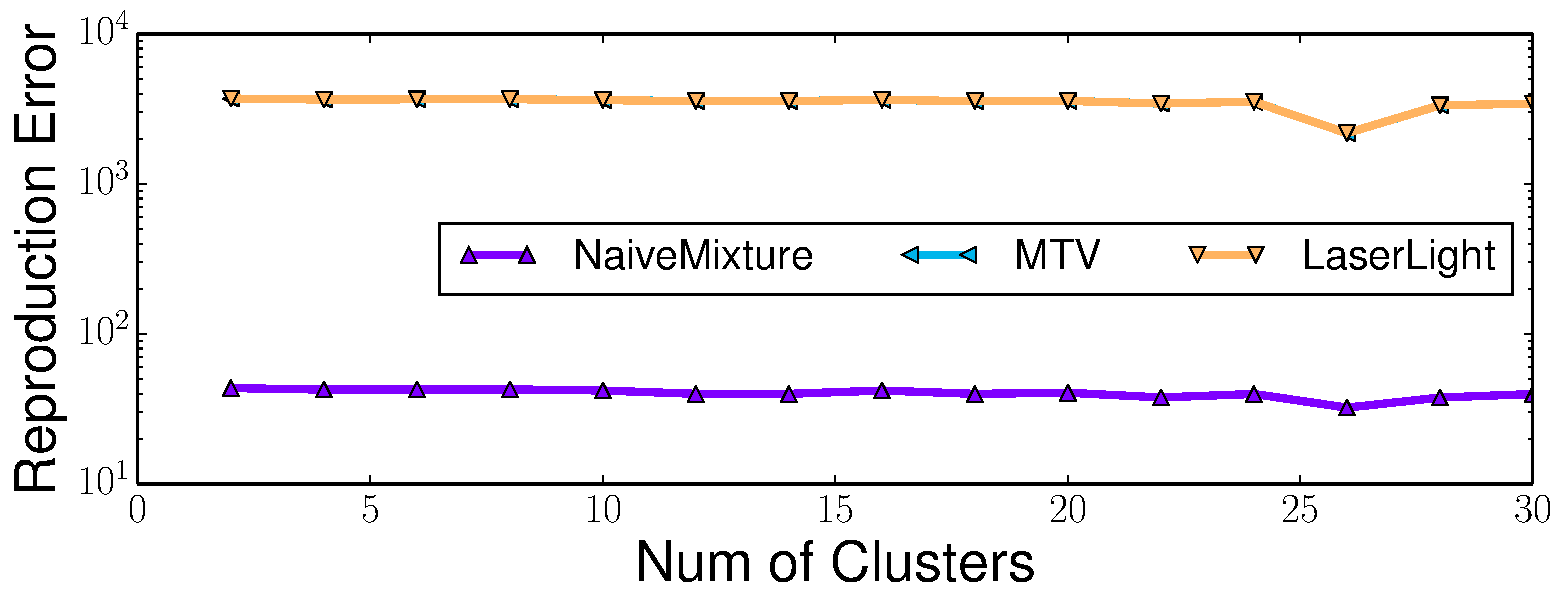
\includegraphics[width=\textwidth]{QueryLogSummarization/graphics/PatternMixtureSummaryErrorComparisonAlone_bankdata.pdf}
     \bfcaption{Naive Mixture v. LaserLight/MTV alone. Note that y-axis is in log scale.}     \label{fig:PatternMixtureEncodingErrorComparisonAlone_bankdata}
    \end{subfigure}
    ~
    \begin{subfigure}[b]{0.47\textwidth}
        \centering       
        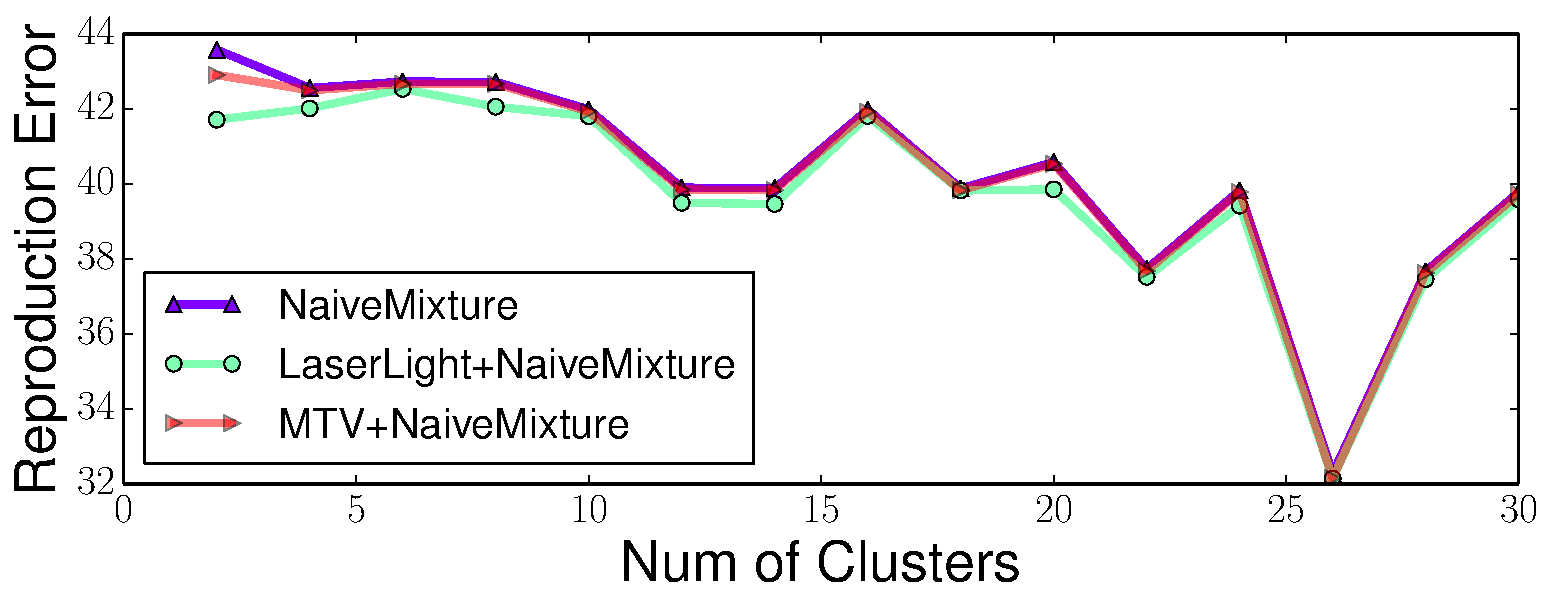
\includegraphics[width=\textwidth]{QueryLogSummarization/graphics/PatternMixtureSummaryErrorComparisonPiggybacking_bankdata.pdf}
     \bfcaption{Naive Mixture v. Naive Mixture+LaserLight/MTV. Note offset in y-axis (non-zero start).}      \label{fig:PatternMixtureEncodingErrorComparisonPiggybacking_bankdata}
    \end{subfigure}
    ~
    \begin{subfigure}[b]{0.47\textwidth}
    \centering       
    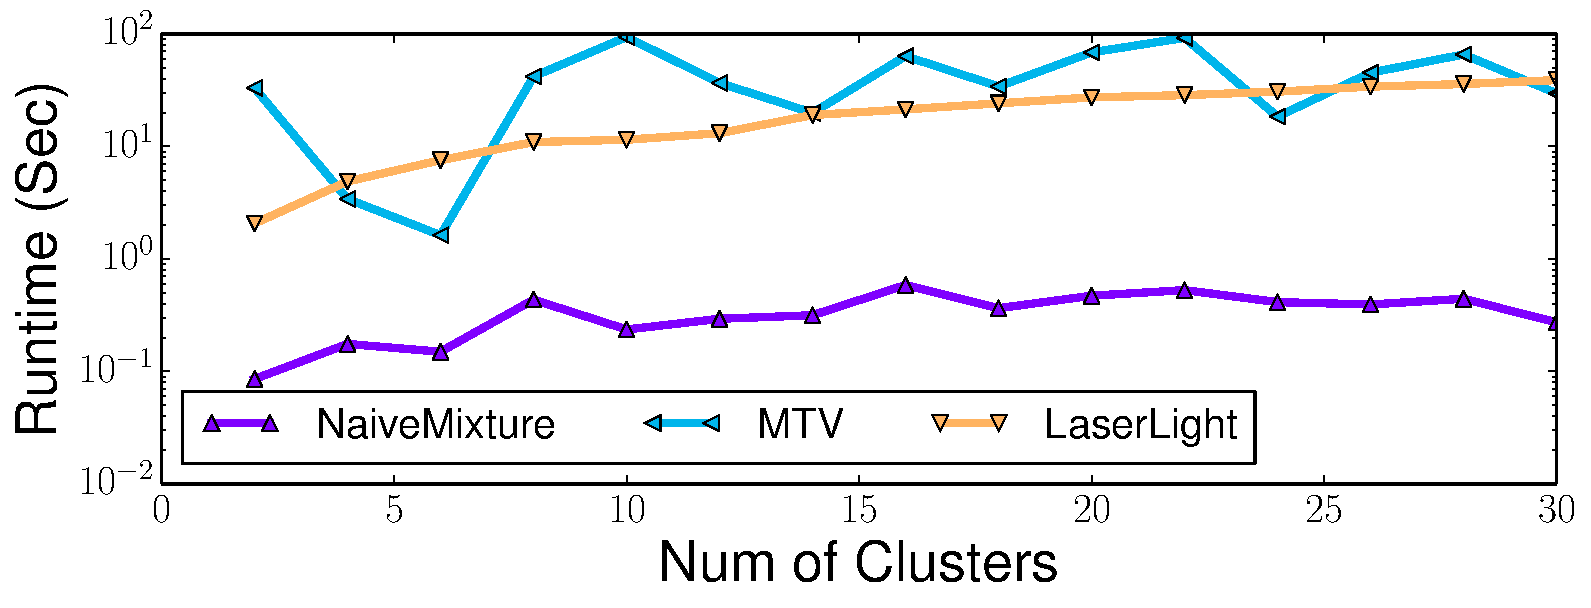
\includegraphics[width=\textwidth]{QueryLogSummarization/graphics/PatternMixtureSummaryRunningTime_bankdata.pdf}
    \bfcaption{Runtime Comparison (y-axis in log scale)}   
    \label{fig:mixtureencodingsrunningtimecomparison_bankdata}
    \end{subfigure}
\bfcaption{Feature-correlation refinement (US bank)}   \label{fig:motivatenaivemixtureencodings_bankdata}
\trimfigurewhitespace
\end{figure}

\subsubsection{Refining Naive Mixture Encodings}
\label{sec:refiningnaivemixtureencodings}
The experiment result is shown in Figure~\ref{fig:PatternMixtureEncodingErrorComparisonPiggybacking_bankdata}.
Note that I offset y-axis to show the change in Error.
We observe from the figure that reduction of Error contributed by plugging-in pattern-based summarizers is small for both algorithms.

\tinysection{Dimensionality Restriction}
For \textit{Laserlight}, the observation is partially due to the fact that I only keep top $100$ features (in terms of variability) of the data as its input, since \textit{Laserlight} is implemented in PostgresSQL 9.1 which has a threshold of $100$ arguments (one argument for each feature) that can be passed to a function.

\tinysection{Pattern Restriction}
For \textit{MTV}, this is due to a runtime error that limits us to $15$ or less patterns.
We refer the reader to Section 4.5 in~\cite{DBLP:journals/tkdd/MampaeyVT12} that explains the difficulty in inferring the maximum entropy distribution constrained by a large number of non-naive patterns.

\begin{figure}[ht!]
	\captionsetup[subfigure]{justification=centering}
    \centering
    \begin{subfigure}[b]{0.48\textwidth}
        \centering       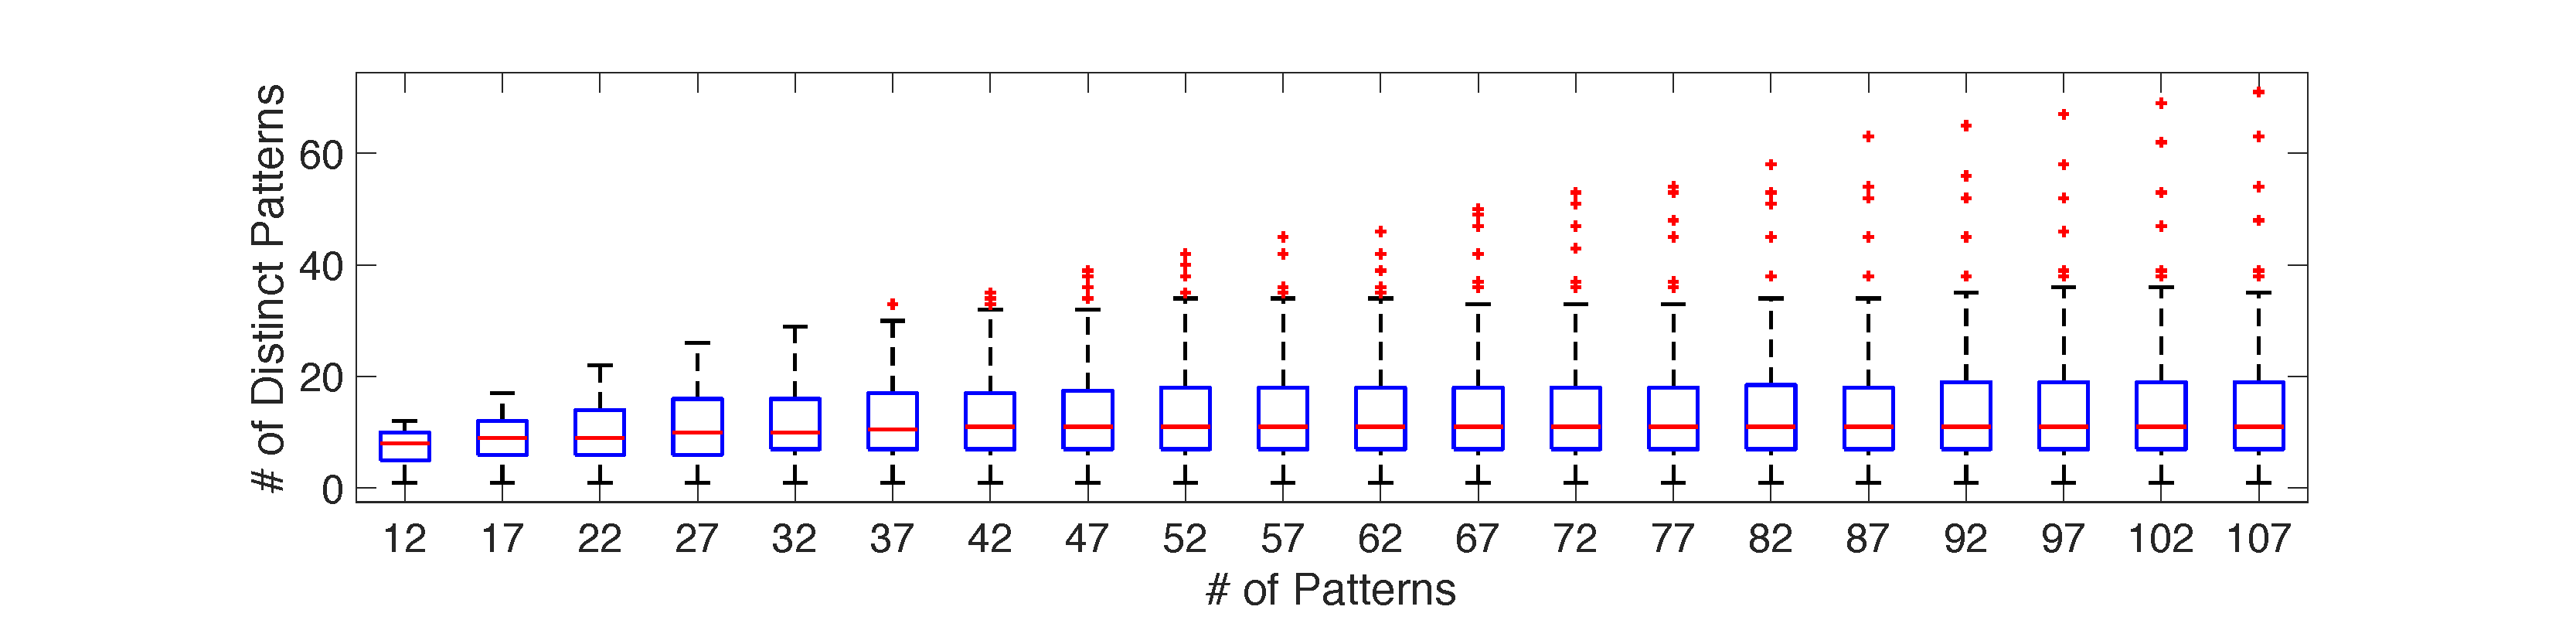
\includegraphics[width=\textwidth]{QueryLogSummarization/graphics/Laserlight_NumDistinctPatternsVNumPatterns.pdf}
 \bfcaption{Laserlight}      \label{fig:patterns_laserlight}
\end{subfigure}
    ~
\begin{subfigure}[b]{0.48\textwidth}
  \centering       
  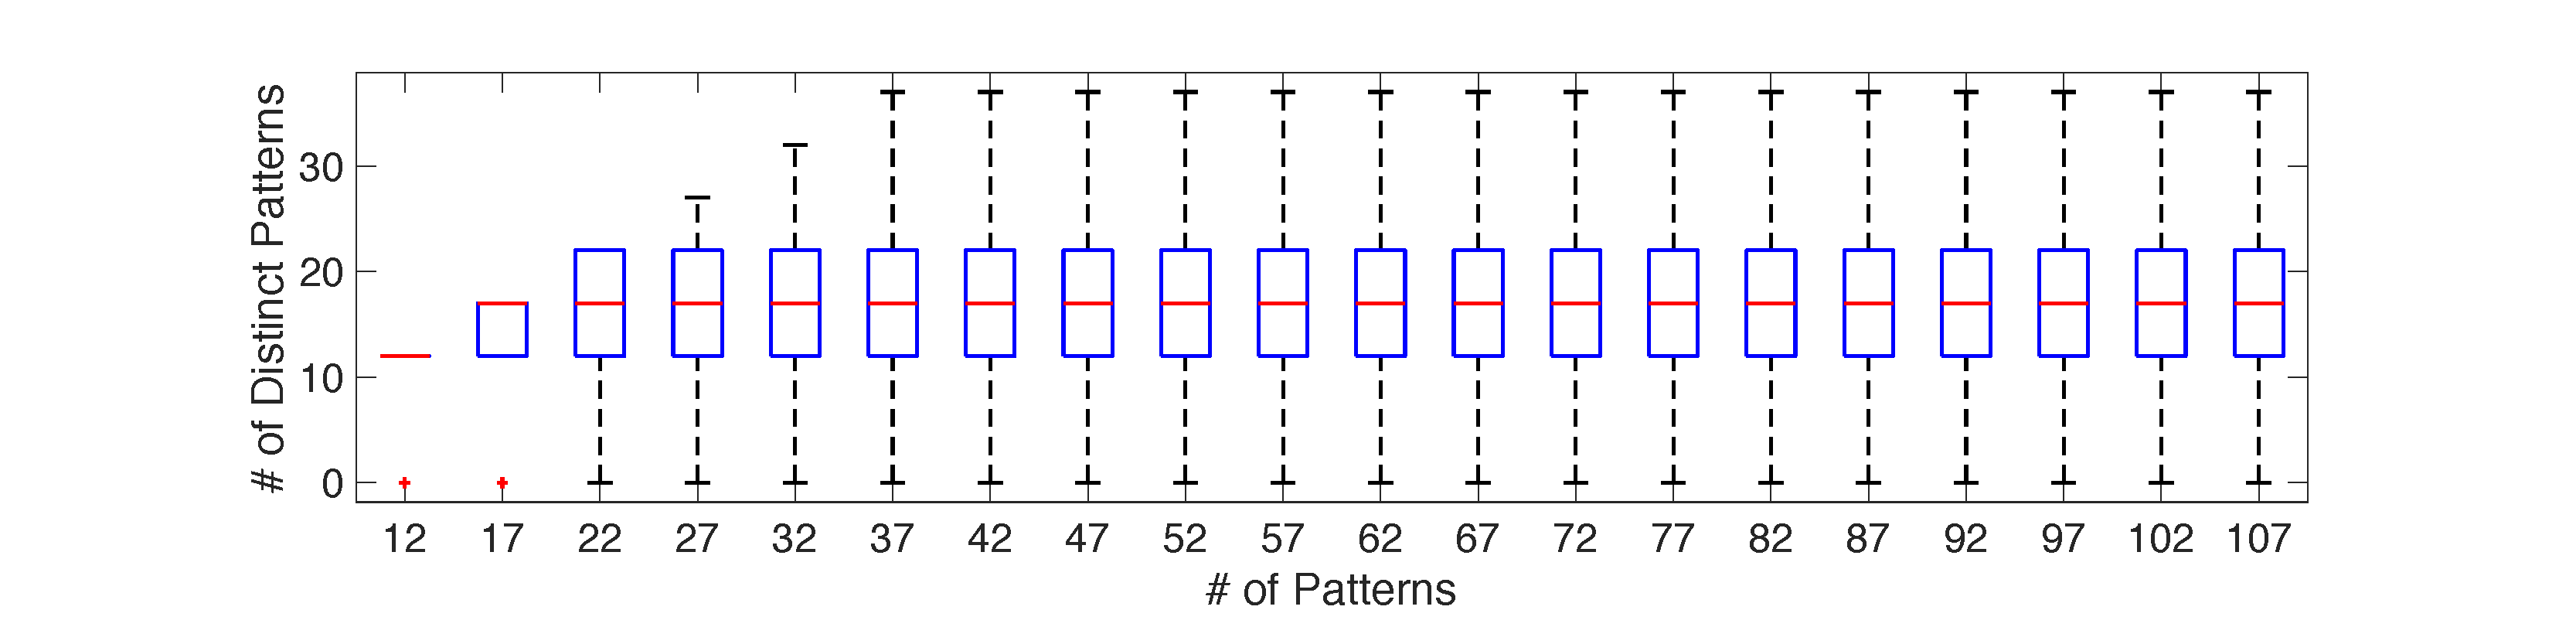
\includegraphics[width=\textwidth]{QueryLogSummarization/graphics/MTV_NumDistinctPatternsVNumPatterns.pdf}
 \bfcaption{MTV}     
 \label{fig:patterns_MTV}
\end{subfigure}
~
\bfcaption{Distinct Patterns v. Number of Patterns }   \label{fig:distinctpatternsofpatternbasedalgorithms}
\trimfigurewhitespace
\end{figure}

\tinysection{Pattern Diversification Failure}
Recall in Section~\ref{sec:naivemixtureencodingrefinement} that pattern diversification can be time-consuming.
As a result, both algorithms implement heuristics that sacrifice the capability of pattern diversification to some extent.
In other words, increase in the total number of patterns mined from \textit{Laserlight} and \textit{MTV} may not lead to commensurate increase in the number of \textit{distinct} patterns (i.e., pattern duplication implies failure in pattern diversification).
Specifically, we run \textit{MTV} and \textit{Laserlight} on each cluster ($30$ clusters in total) and vary the number of patterns configured for mining from $12$ to $107$.
We collect the number of \textit{distinct} patterns that they have mined as well as the running time under each configuration.
The experiment result is shown in Figure~\ref{fig:distinctpatternsofpatternbasedalgorithms} where y-axis is the number of distinct patterns and x-axis is the total number of patterns mined through \textit{Laserlight} and \textit{MTV}.
We observe that \textit{Laserlight} and \textit{MTV} fail to extensively explore hidden feature-correlation in our chosen datasets.

\begin{figure}[ht!]
	\captionsetup[subfigure]{justification=centering}
    \centering
    \begin{subfigure}[b]{0.48\textwidth}
        \centering       
        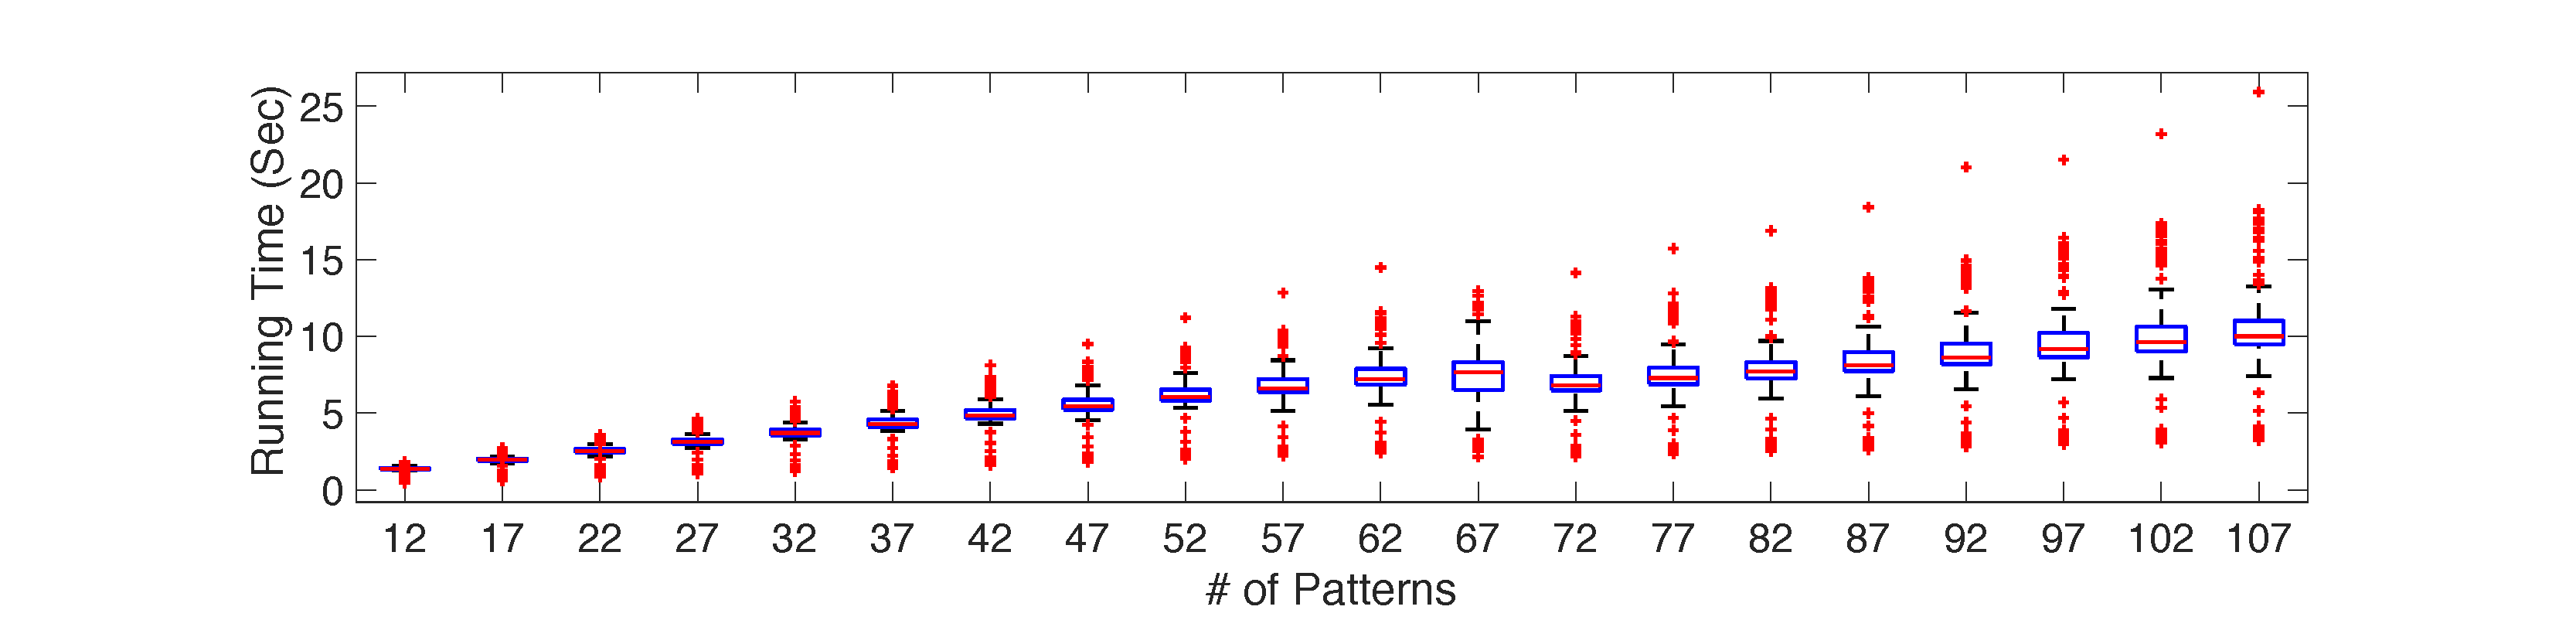
\includegraphics[width=\textwidth]{QueryLogSummarization/graphics/Laserlight_RunningTimeVNumPatterns.pdf}
 \bfcaption{Laserlight}      
 \label{fig:runningtime_laserlight}
\end{subfigure}
    ~
\begin{subfigure}[b]{0.48\textwidth}
  \centering       
  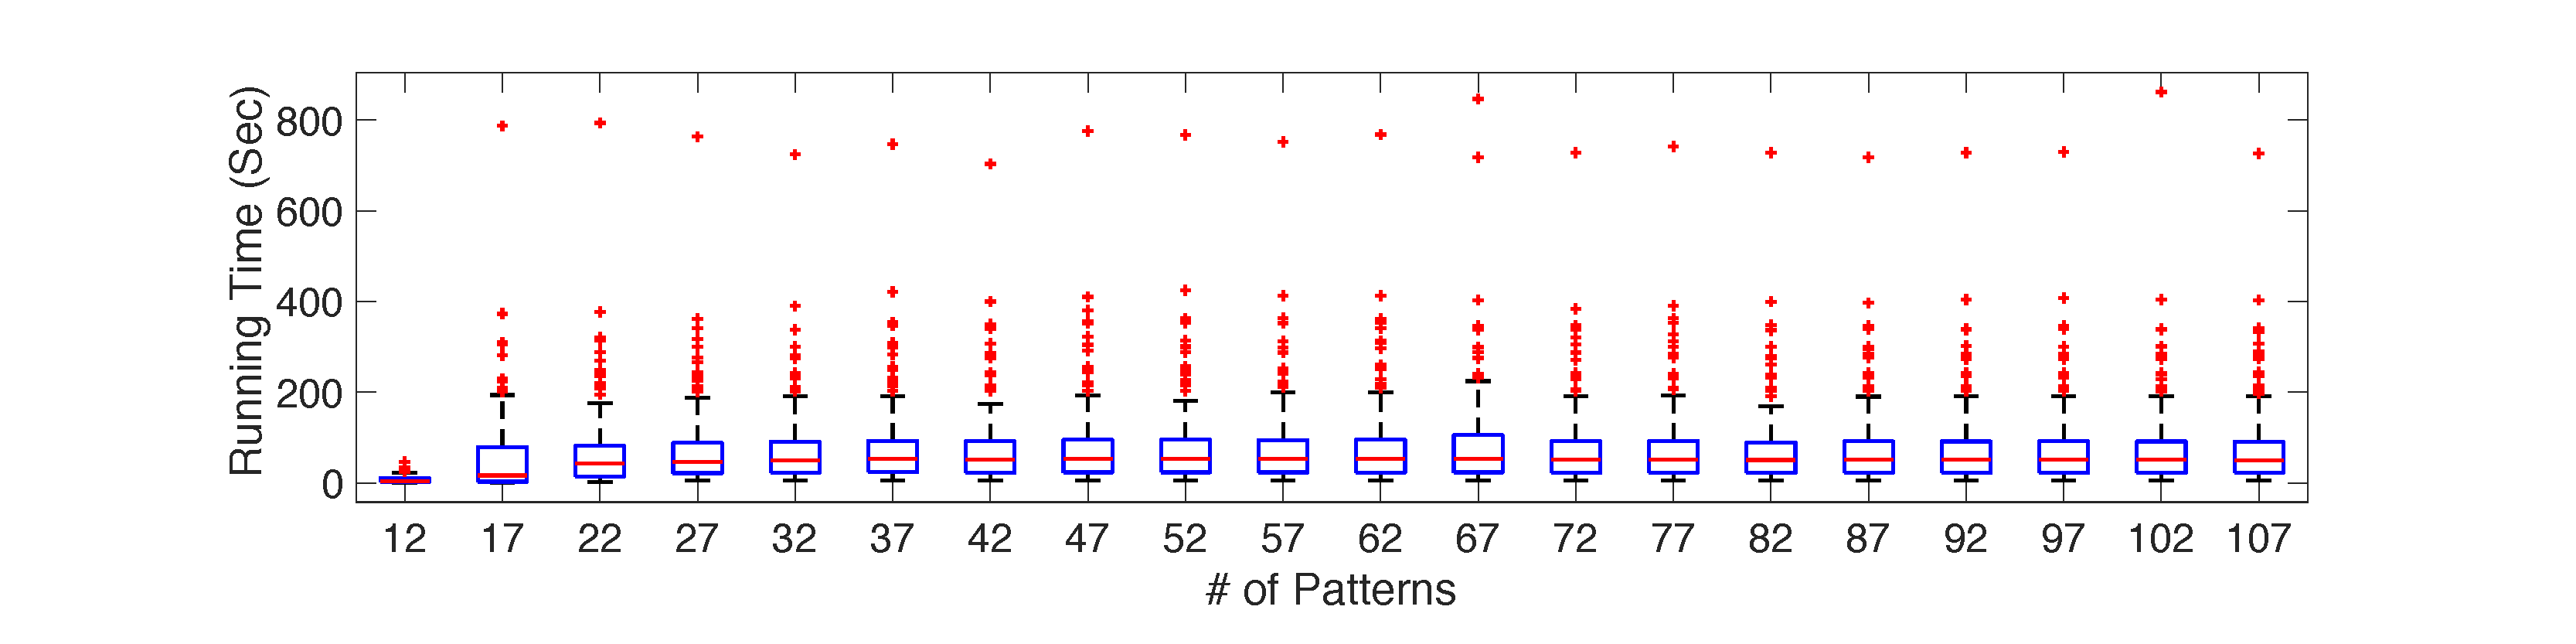
\includegraphics[width=\textwidth]{QueryLogSummarization/graphics/MTV_RunningTimeVNumPatterns.pdf}
 \bfcaption{MTV}     
 \label{fig:runningtime_MTV}
\end{subfigure}
~
\bfcaption{Running Time v. Number of Patterns}   \label{fig:runningtimeofpatternbasedalgorithms}
\trimfigurewhitespace
\end{figure}

\tinysection{Time Restriction}
Computation efficiency will also influence effectiveness of pattern based summarizers when it takes too long to mine a potentially large set of informative patterns under from the data.
The experiment result for running time analysis is shown in Figure~\ref{fig:runningtimeofpatternbasedalgorithms}.
We observe that \textit{Laserlight} shows a close-to-linear growth rate.
For \textit{MTV} the running time spikes at $17$ patterns and remains oscillating between high levels afterwards.


\section{Alternative Applications}
\label{sec:evaluatingalternativeapplications}
% !TEX root = ../paper.tex
To fairly evaluate \textit{Laserlight} and \textit{MTV}, I incorporate their own data sets and empirically evaluate them against \textit{naive mixture encoding} under their own applications.

\tinysection{Data Sets}
Specifically, I choose \textit{Mushroom} data set used in \textit{MTV}~\cite{DBLP:journals/tkdd/MampaeyVT12} which is obtained from FIMI dataset repository and U.S. Census data on Income or simply \textit{Income} data set, which is downloaded from IPUMS-USA at \textit{https://usa.ipums.org/usa/} and used in \textit{Laserlight}~\cite{DBLP:journals/pvldb/GebalyAGKS14}.
The basic statistics of the data sets are given in Table~\ref{table:extendeddatasummary}.

\begin{table}[h!]
\centering
\bfcaption{Data Sets of Alternative Applications}
\label{table:extendeddatasummary}
{\small \centering
\begin{tabular}{c c c}
\toprule
Statistics & Income & Mushroom \\
\midrule
\# Distinct data tuples & 777493 & 8124\\
\midrule
\# Features per tuple & 9 & 21\\
\midrule
Feature Binary-valued? & no& no\\
\midrule
\# Distinct features & 783 & 95\\
\midrule
Binary Classification Feature & $>100,000$? & Edibility\\
\midrule
Assumed data tuple multiplicity & 1 & 1\\
\bottomrule
\end{tabular}
}
\end{table}

\subsection{Experiments}
\label{sec:evaluatingalternativeapplicationsexperiments}
All experiments involving \textit{Laserlight} and \textit{MTV} will be evaluated under their own Error measures and data sets, unless otherwise stated.
The experiments are organized as follows: First, we establish baselines by evaluating classical \textit{Laserlight} and \textit{MTV} on their original data; Then we show that classical \textit{Laserlight} and \textit{MTV} can be generalized to partitioned data and that the generalization improves on their Error measures and also runtime; At last, we compare their generalized versions with \textit{naive mixture encoding} to show that \textit{naive mixture encoding} is a reasonable alternative.% in terms of run time and Error.

\subsubsection{Error Measures}
We first explain how \textit{naive mixture encoding} is evaluated based on Error defined by \textit{Laserlight} and \textit{MTV}.

\tinysection{Evaluating Naive Encoding on Laserlight Error}
Algorithm \textit{Laserlight} summarizes data $D$ which consists of feature vectors $t$ augmented by some binary feature $v$.
Denote the valuation of the binary feature $v$ for each feature vector $t$ as $v(t)$. 
The goal is to mine a summary encoding $\encoding$, which is a set of patterns contained in $t\in D$ that offer predictive power on $v(t)$.
Denote the estimation (based on $\encoding$) of $v(t)$ as $u_{\encoding}(t)\in [0,1]$, the \textit{Laserlight} Error is measured by $$\sum_t ( v(t)\log(\frac{v(t)}{u_{\encoding}(t)})+(1-v(t))\log(\frac{1-v(t)}{1-u_{\encoding}(t)}) )$$
Since \textit{naive encoding} $\naiveencoding$  assumes feature independence, estimation of $v(t)$ is independent of $t$, namely $u_{\naiveencoding}(t)=u_{\naiveencoding}=|\{\tau|v(\tau)=1,\tau\in D\}|/|D|$.
Consequently, the \textit{Laserlight} Error of \textit{naive encoding} is $$-|D|(u_{\naiveencoding}\log u_{\naiveencoding}+(1-u_{\naiveencoding})\log (1-u_{\naiveencoding}) )$$

\tinysection{Evaluating Naive Encoding on MTV Error}
Given binary feature vectors $D$, the \textit{MTV} Error of encoding $\encoding$ is $$-|D|H(\overline{\rho}_\encoding)+1/2|\encoding|\log|D|$$ where $H(\overline{\rho}_\encoding)$ is the entropy of maximum entropy distribution $\overline{\rho}_\encoding$ defined in Section~\ref{sec:maximumentropydistribution}.
The second term in \textit{MTV} Error penalizes Verbosity of the encoding $\encoding$.
Since naive encoding assumes feature independence, we can first compute entropy of the marginal distribution of each individual feature.
Entropy $H(\overline{\rho}_\encoding)$ is simply the sum of feature entropies.

\tinysection{Evaluating Naive Mixture Encoding}
Evaluation of \textit{naive encoding} can be generalized to \textit{naive mixture} by taking a weighted average over resulting clusters (See Section~\ref{sec:generalizedinformationlossmeasures}).

\begin{figure}[ht!]
    \captionsetup[subfigure]{justification=centering}
    \centering
    \begin{subfigure}[b]{0.48\textwidth}
        \centering       
        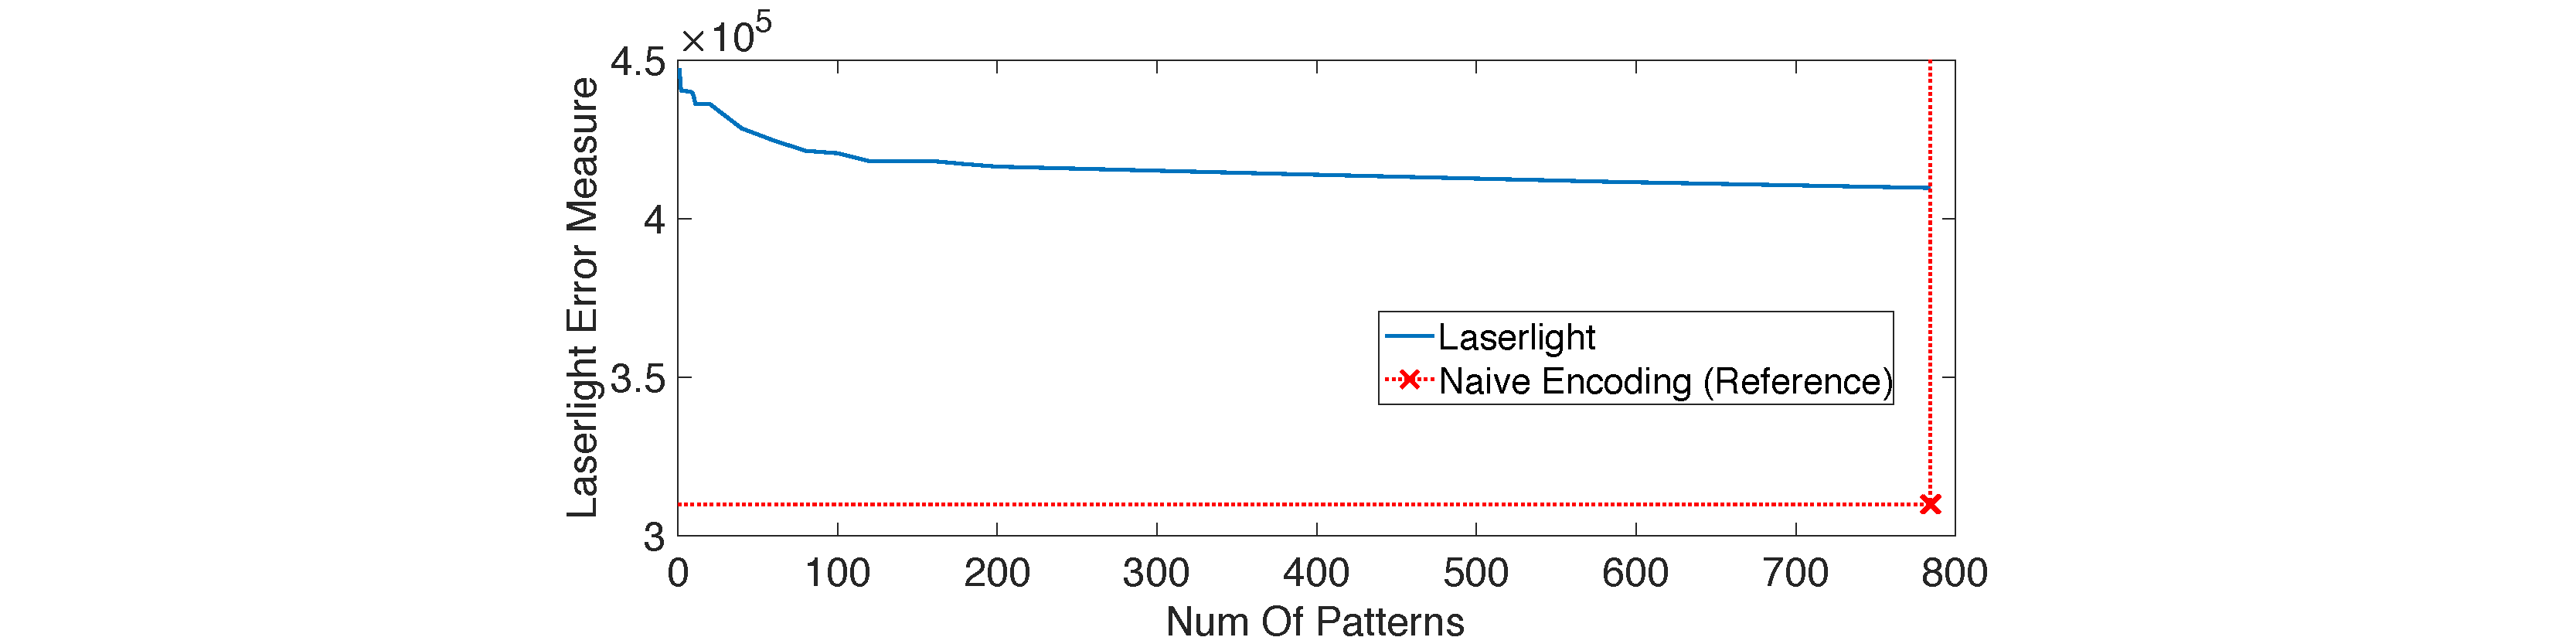
\includegraphics[width=\textwidth]{QueryLogSummarization/graphics/Laserlight_Error_vs_NumOfPatterns.pdf}
        \bfcaption{Laserlight Error v. \# of Patterns on Income data}
        \label{fig:Laserlight_Error_vs_NumOfPatterns}
    \end{subfigure}
    ~
    \begin{subfigure}[b]{0.48\textwidth}
        \centering       
        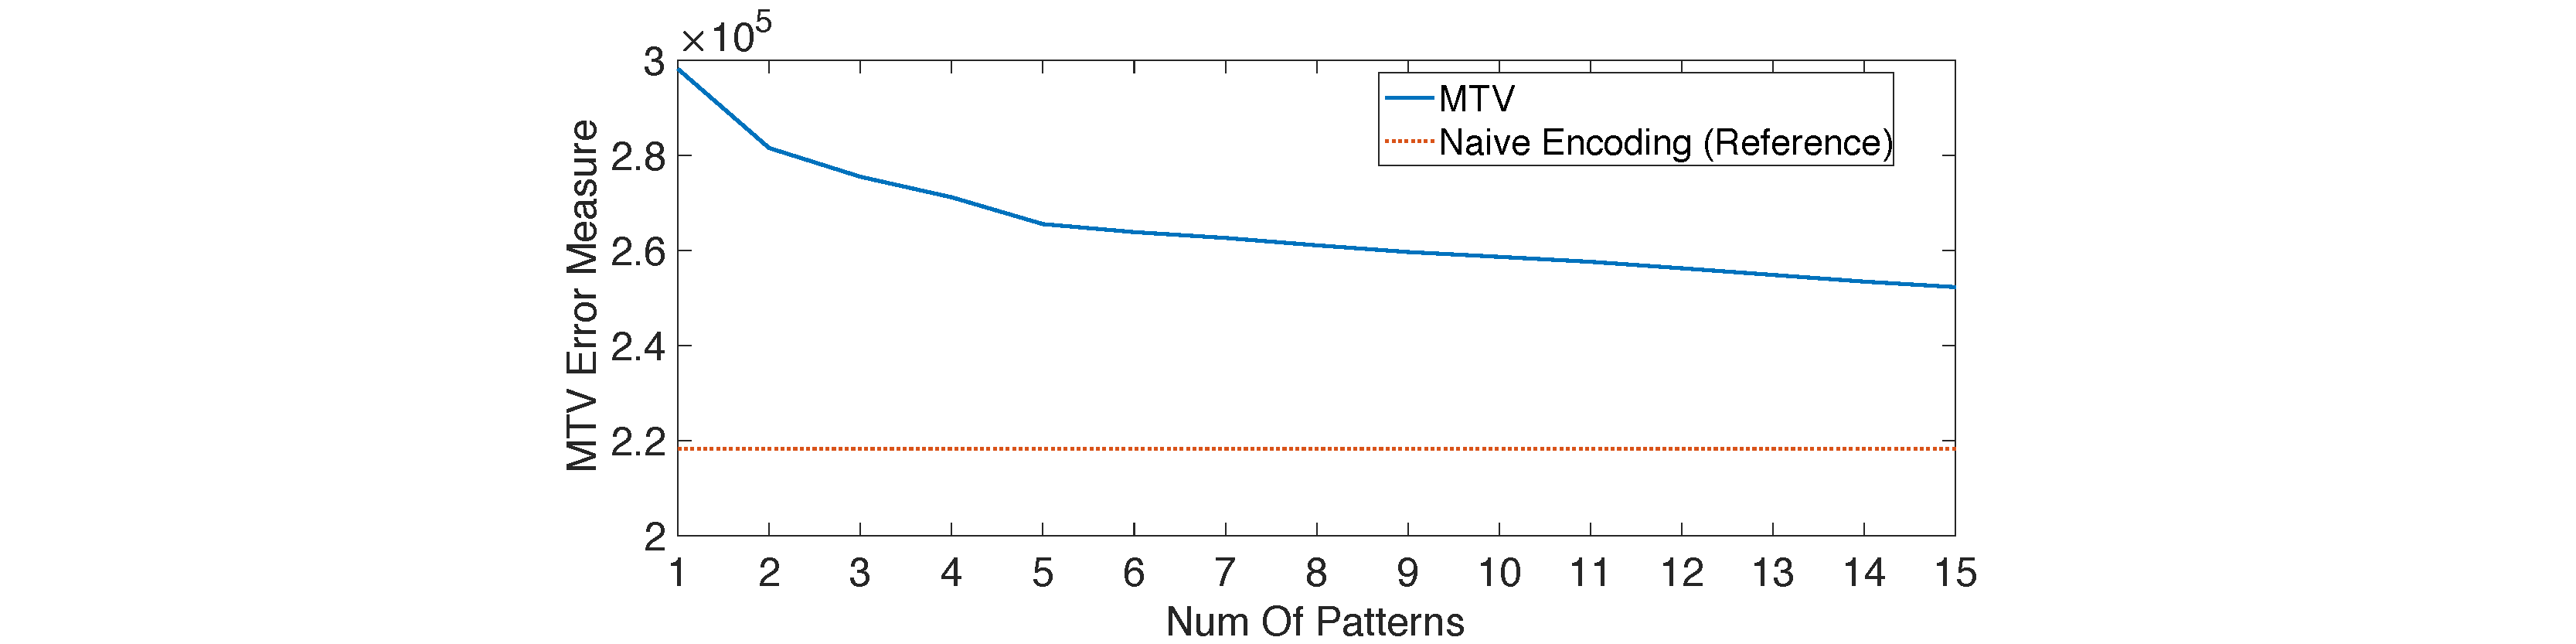
\includegraphics[width=\textwidth]{QueryLogSummarization/graphics/MTV_Error_vs_NumOfPatterns.pdf}
        \bfcaption{MTV Error v. \# of Patterns on Mushroom data}     
        \label{fig:MTV_Error_vs_NumOfPatterns}
    \end{subfigure}
    ~
    \bfcaption{Error v. Number of Patterns. Note: non-zero start of y-axis.}   
    \label{fig:performance_vs_num_of_patterns}
    \trimfigurewhitespace
\end{figure}

\subsubsection{Classical Laserlight and MTV}
\label{sec:classicallaserlightandmtv}

\tinysection{Establishing Baselines} 
To establish baselines, we evaluate \textit{Laserlight} and \textit{MTV} on their own data sets.
The take-aways from related experiments are that (1) \textit{naive encoding} is faster and more accurate than classical \textit{Laserlight} and \textit{MTV}; (2) the runtime increases superlinearly with the number of patterns mined from both \textit{Laserlight} and \textit{MTV}.

\tinysection{Dimentionality Reduction}
Recall in Section~\ref{sec:refiningnaivemixtureencodings} that \textit{Laserlight} is restricted to $100$ features.
For its own \textit{Income} data set, \textit{Laserlight} can be applied with its full set of $783$ features.
This is due to the prior knowledge that the $783$ features belong to $9$ groups.
In each group, features are mutually exclusive which can be reduced to a single feature.
Similarly, \textit{Mushroom} data set can be reduced from $95$ to $21$ features (See Table~\ref{table:extendeddatasummary}).

The results related to Error measures are given in Figure~\ref{fig:performance_vs_num_of_patterns}.
X-axis is the number of patterns and y-axis represents the Error measure of \textit{Laserlight} and \textit{MTV} in Figure~\ref{fig:Laserlight_Error_vs_NumOfPatterns} and~\ref{fig:MTV_Error_vs_NumOfPatterns} respectively.
We incorporate \textit{naive encoding} in Figure~\ref{fig:Laserlight_Error_vs_NumOfPatterns} as the reference method.
Since there are $784$ total number of features for \textit{Income} data set, the verbosity of \textit{naive encoding} will be $784$, which is shown as vertical dotted line in Figure~\ref{fig:Laserlight_Error_vs_NumOfPatterns}.
For \textit{Mushroom} data set, the verbosity of its \textit{naive encoding} will be $96$.
However, \textit{MTV} quits with error message if it is requested to mine over $15$ patterns.
Hence for Figure~\ref{fig:MTV_Error_vs_NumOfPatterns}, the limit of x-axis is $15$ and we only show Error of \textit{naive encoding} as a reference line without marking out its verbosity. 
We observe in Figure~\ref{fig:Laserlight_Error_vs_NumOfPatterns} that \textit{naive encoding} outperforms \textit{Laserlight} when their verbosity is equal (i.e., $784$).
In addition, after $100$ patterns, the slope of Error reduction becomes relatively flat.
Similar observation can be made from Figure~\ref{fig:MTV_Error_vs_NumOfPatterns}.

\begin{figure}[h!]
	\captionsetup[subfigure]{justification=centering}
    \centering

    \begin{subfigure}[b]{0.48\textwidth}
        \centering       
        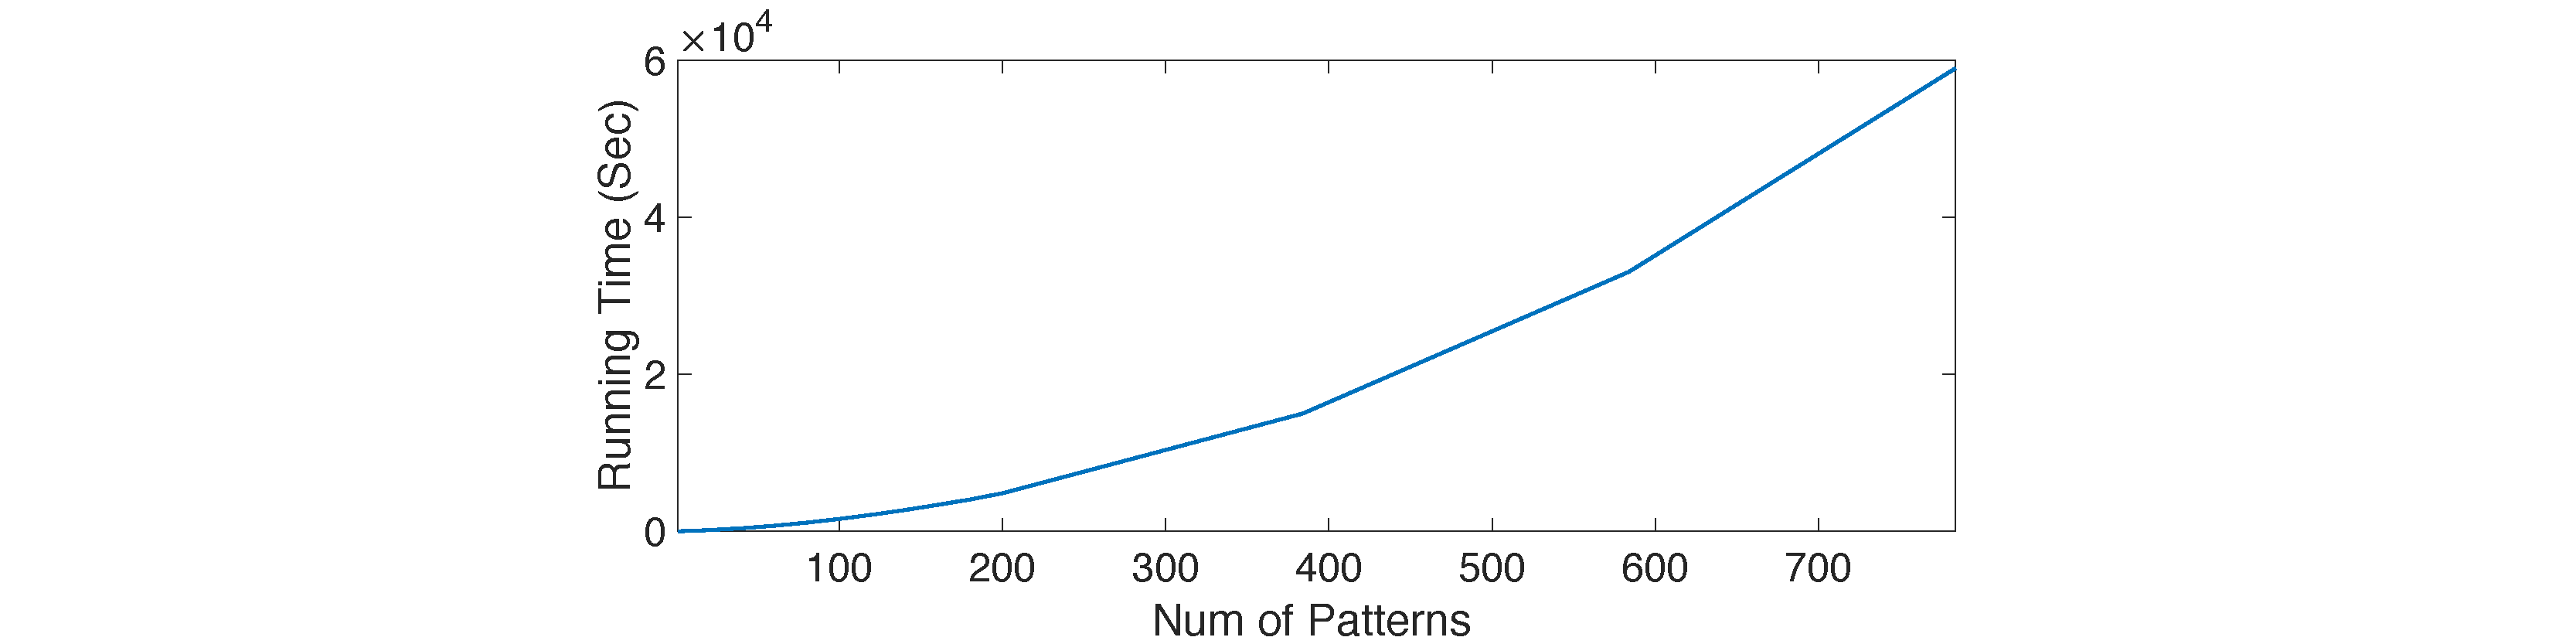
\includegraphics[width=\textwidth]{QueryLogSummarization/graphics/Laserlight_runningTimes_vs_NumOfPatterns.pdf}
 \bfcaption{Laserlight Running Time on Income Data}      \label{fig:laserlight_runningTimes_vs_NumOfPatterns}
\end{subfigure}
    ~
     \begin{subfigure}[b]{0.48\textwidth}
        \centering       
        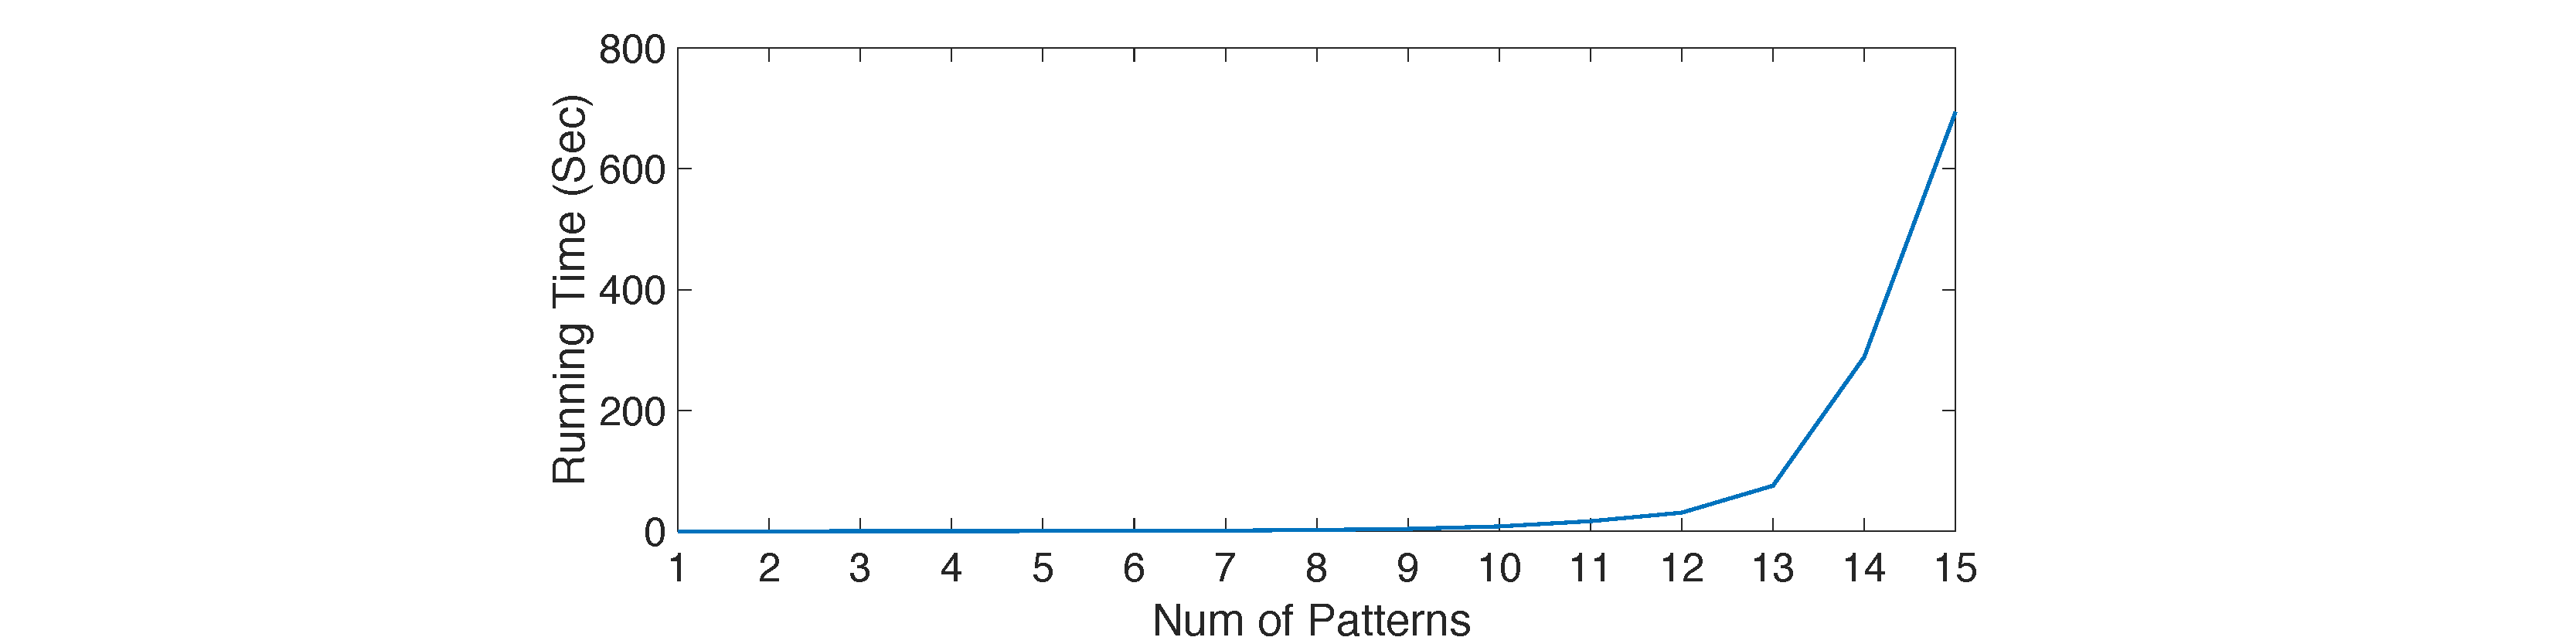
\includegraphics[width=\textwidth]{QueryLogSummarization/graphics/MTV_runningTimes_vs_NumOfPatterns.pdf}
 \bfcaption{MTV Running Time on Mushroom data}      \label{fig:mtv_runningTimes_vs_NumOfPatterns}
\end{subfigure}
    ~   
\bfcaption{Running Time of Laserlight and MTV}   \label{fig:runningTime_analysis}
\trimfigurewhitespace
\end{figure}

Next I show corresponding run time results in Figure~\ref{fig:runningTime_analysis}.
We observe that the running time increases exponentially with the number of patterns, for both \textit{Laserlight} and \textit{MTV}.

\subsubsection{Generalizing Laserlight and MTV}
\label{sec:generalizinglaserlightandmtv}
In this section, we generalize \textit{Laserlight} and \textit{MTV} on partitioned data by applying them on each cluster.
We then combine Errors on all clusters by taking a weighted average, as described in Section~\ref{sec:generalizedinformationlossmeasures}.
Depending on how many patterns are mined from each cluster, \textit{Laserlight} and \textit{MTV} can be generalized into two types: (1) The number of patterns mined from each cluster is scaled to be equal to Verbosity of the \emph{naive encoding}; and (2) The total number of patterns mined from all clusters is fixed to a given number.
I name the first type \emph{Laserlight (MTV) Mixture Scaled}, which is comparable to \emph{naive mixture encoding}.
I name the second type \emph{Laserlight (MTV) Mixture Fixed}, which is comparable to the classical \emph{LaserLight (MTV)} algorithm.

\tinysection{Take-away}
As the data is partitioned into more clusters, both runtime and Error of \emph{Laserlight (MTV) Mixture Fixed} exponentially decrease.
This observation can be potentially generalized to other pattern mining algorithms.
For experiment details, I refer the reader to~\cite{DBLP:journals/corr/abs-1809-00405}.

\begin{figure}[h!]
	\captionsetup[subfigure]{justification=centering}
    \centering
    \begin{subfigure}[b]{0.47\textwidth}
        \centering       
        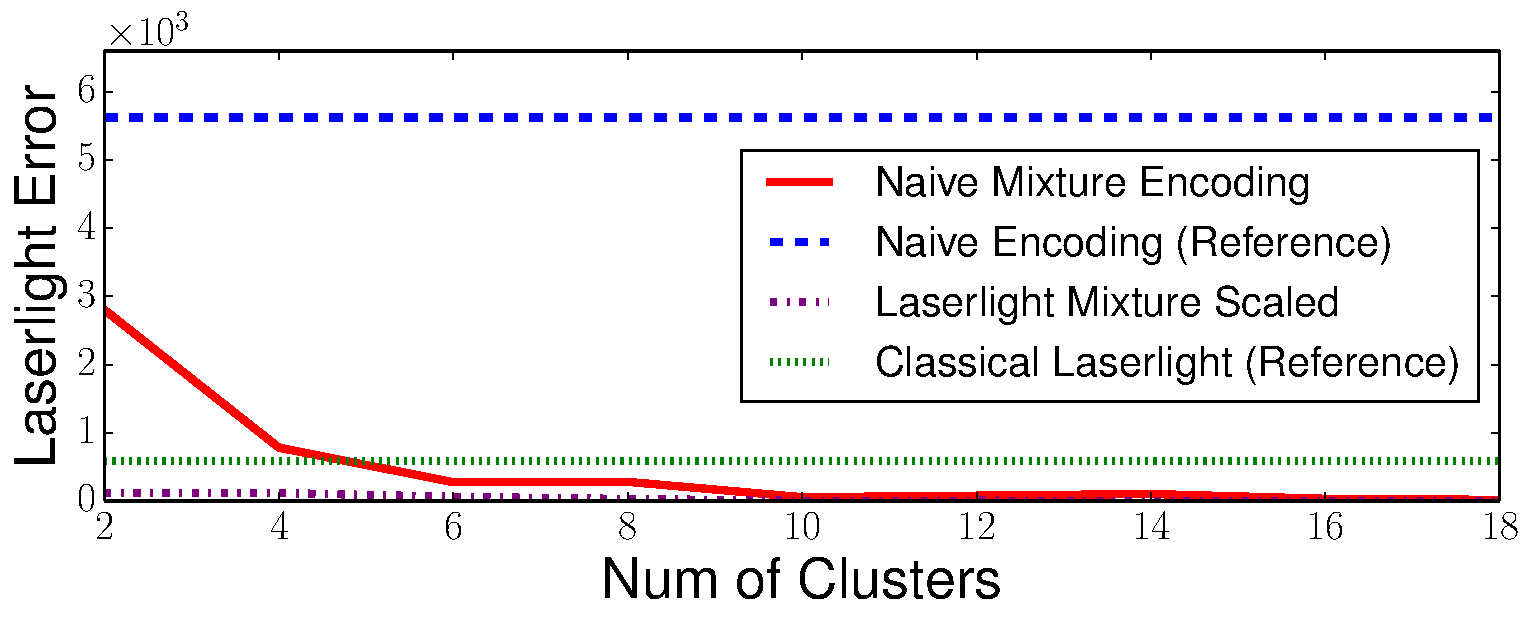
\includegraphics[width=\textwidth]{QueryLogSummarization/graphics/Laserlight_Errors_vs_NumOfClusters.pdf}
 \bfcaption{Laserlight Error v. \# of Clusters on Mushroom data}      \label{fig:LaserlightMixture_Errors_vs_NumOfClusters}
\end{subfigure}
    ~
\begin{subfigure}[b]{0.47\textwidth}
  \centering       
  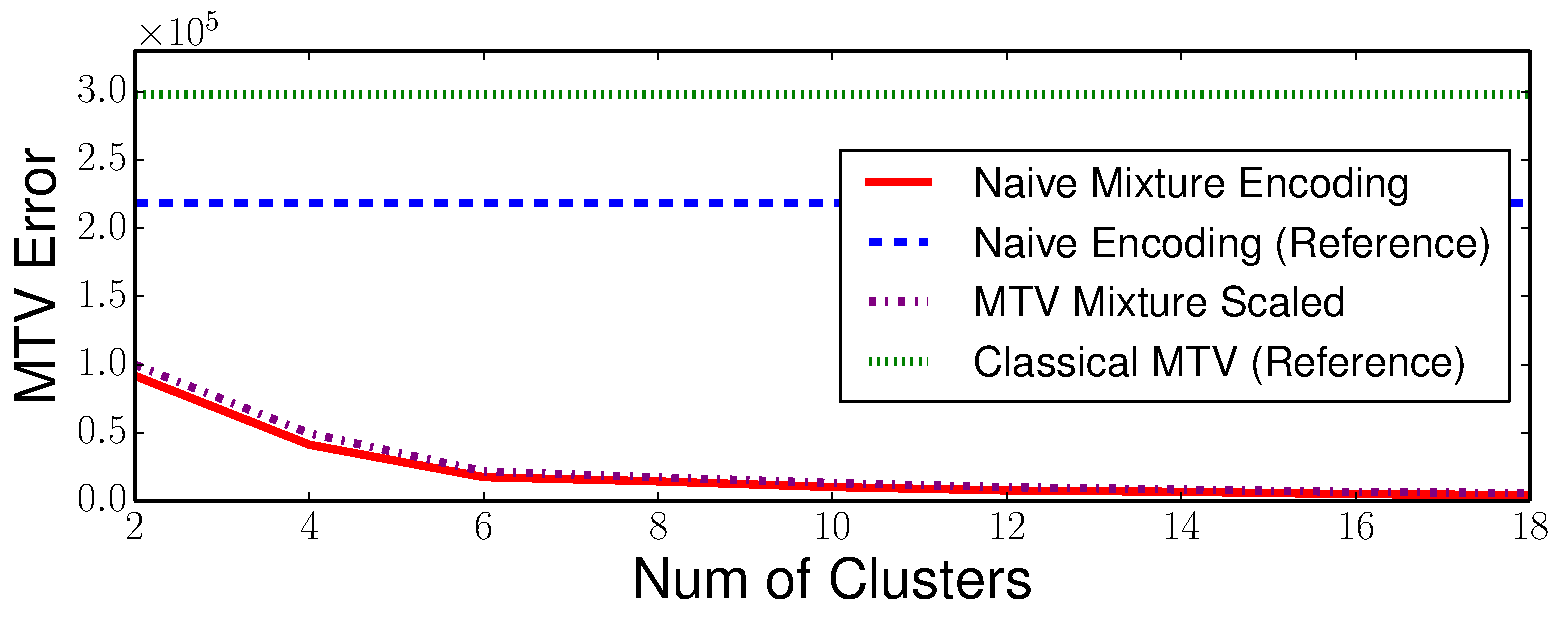
\includegraphics[width=\textwidth]{QueryLogSummarization/graphics/MTV_Error_vs_NumOfClusters.pdf}
 \bfcaption{MTV Error v. \# of Clusters on Mushroom data}     
 \label{fig:MTVMixture_vs_Laserlight_runningTimes_IncomeData}
\end{subfigure}
~
\bfcaption{Naive Mixture v. Laserlight/MTV Mixture}   
\label{fig:Naive Mixture Encoding_vs_Laserlight&MTV_Mixture}
\trimfigurewhitespace
\end{figure}
\subsubsection{Comparison with Naive Mixture Encoding}
\label{sec:Evaluating_Naive_Mixture_Encoding}

At last, we compare \emph{Laserlight (MTV) Mixture Scaled} with \emph{naive mixture encoding}.
Note that it is time-consuming for \emph{Laserlight} to mine the same number of patterns as \emph{naive encoding} on \emph{Income} data (See runtime analysis in~\cite{DBLP:journals/corr/abs-1809-00405}), I choose \emph{Mushroom} data for \emph{Laserlight Mixture Scaled} instead.
The experiment results are given in Figure~\ref{fig:Naive Mixture Encoding_vs_Laserlight&MTV_Mixture}. 
The x-axis for all sub-figures in Figure~\ref{fig:Naive Mixture Encoding_vs_Laserlight&MTV_Mixture} represents the number of clusters and the y-axes stands for \emph{Laserlight} and \emph{MTV} Error respectively.
I incorporate baselines (i.e., \emph{naive encoding}, classical \emph{Laserlight} and \emph{MTV}) as reference lines in Figure~\ref{fig:LaserlightMixture_Errors_vs_NumOfClusters} and~\ref{fig:MTVMixture_vs_Laserlight_runningTimes_IncomeData} respectively.
We also experienced a limitation of $15$ patterns for \emph{MTV}.
Hence the comparison between \emph{MTV Mixture Scaled} and {naive mixture encoding} is not strictly on equal footing as \emph{MTV Mixture Scaled} is not able to reach the same Total Verbosity as \emph{naive mixture encoding}.
Note that their difference in Verbosity is mitigated by the fact that \emph{MTV} Error measure penalizes encoding Verbosity.

Figure~\ref{fig:LaserlightMixture_Errors_vs_NumOfClusters} shows that both \emph{naive mixture encoding} and \emph{Laserlight Mixture Scaled} have lower Error than their baselines.
In addition, \emph{Laserlight Mixture Scaled} has lower Error than \emph{naive mixture encoding} when the number of clusters is less than $4$ and they become close after $6$ clusters.
In other words, \emph{Laserlight} is more accurate on lightly partitioned data. 
As the data is further partitioned, clusters become easier to summarize, and \emph{naive encoding} becomes more similar to \emph{Laserlight}.
Figure~\ref{fig:MTVMixture_vs_Laserlight_runningTimes_IncomeData} shows that \emph{naive mixture encoding} marginally outperforms \emph{MTV Mixture Scaled}.

\tinysection{Take-away}
\emph{Naive mixture encoding} is faster and has similar (lower) Error than \emph{Laserlight (MTV) Mixture Scaled}.


%\section{Related Work}
%\label{sec:backgroundandrelatedwork}
%% !TEX root = ../paper.tex
%The focus of this paper is to model user intents via query monitoring. Provided that an accurate model can be created, it would lead not only to effective insider attack detection systems, but could have implications for other fields like database performance optimizers.

%There are some upfront security policies used and enforced in organizations to protect the integrity and confidentiality of the resources.
%For instance, as a multi-level security (MLS) policy, \textit{Bell-LaPadula}~\cite{bellLaPadula} has very rigid constraints, and does not tolerate normal changes in business needs over time. Policies like the \textit{Chinese Wall Security Model}~\cite{ChineseWall} focus on preventing conflicts of interest in a commercial domain rather than explicitly protecting resources. A more permissive approach is based on role-based access control (RBAC)~\cite{rolebased}, where predetermined user groups are permitted to perform specific tasks.  However, even here, the specific tasks performed by each group might evolve over time.%There are also security policies especially tailored for preventing insider attacks~\cite{pramanik2004security} and enforcing policies~\cite{enforceable2000}. 
%Although useful, these policies cannot prevent insider attacks as there are often policy violations and exceptions in the implementation~\cite{bishop2010risk}. These exceptions can be explained with the \textit{Oracle Policy}, \textit{Feasible Policy} and \textit{Configuration Policy} concepts~\cite{bishop2010risk}. \textit{Oracle Policy} represents the ideal case which is what the policy maker actually intends with the policy. It can be non-deterministic but it supplies a correct answer for any question asked as it covers the intent and custom. \textit{Feasible Policy} substitutes the ideal case with an implementation of it on a computer system. Lastly, \textit{Configuration Policy} expresses the application of the \textit{Feasible Policy} on a particular system. This means that the ideal case expressed in the policy may not always be enforced on the computer system.

%The basic idea behind \sysname{} is to profile normal user behavior, detect suspicious behavior using this information, and distinguish malicious behavior from benign intents~\cite{Kul2015Jowua}. 
%Indeed, this idea is not new; there are many anomaly detection systems focusing on suspicious behavior of users.  
%Specific examples include file access~\cite{wang2016fileaccess} and transfers~\cite{Arief2015Jowua}, online and social behavior~\cite{Gavai2015Jowua}, activities on a website~\cite{manavoglu2003network}, command-line statements~\cite{maxion2002masquerade} and SQL queries issued to a database~\cite{Mathew2010Raid}. 

%\textbf{SQL queries as a resource:}
%As the basic unit of interaction between a database and its users, the sequence of SQL queries that a user issues effectively models the user's behavior. Also, queries that are similar in nature imply that they might be issued to perform similar duties. Hence, auditing SQL query logs of the databases and having a sense of what the query intends to do correctly gains a lot of importance.

%\textit{Query interpretation} is the problem of understanding the goal of the query and it is regarded as hard as writing a new query as the complexity of the query increases~\cite{gatterbauer2011databases}. QueryViz~\cite{Danaparamita2011queryviz} addresses this problem by visualizing the query. It takes SQL query and the schema of the database; and parses the query, builds an AST and creates a graph for users to view it. The aim is to present queries as simple as possible for the users to understand them, as it is easier to understand the relationships and references in a query when it is graphically visualized.

%However, it is more practical to analyze large SQL query logs as a whole. Generating query cluster visualizations is still a complex task considering that even visualizing just one query accurately to help users understand the intent behind the query quickly is still a research challenge~\cite{gatterbauer2011databases}. 

%The authors of~\cite{Kamra2007SyntaxBased} focus on detection of potential intrusions on database systems. In their paper, they introduce a mechanism which analyzes audit logs of databases with both defined user roles and undefined user roles. This system uses multiple techniques to attempt to detect the threats depending on the role distinction and builds user profiles.
%For representing their data, the authors use a quiplet relation. This relation contains data bases on the command, the projection data, and the selection data. To further expand on this data representation, the authors use fine, medium, and coarse-quiplets, with less data represented in the respective relations. In a Role Based Access Control (RBAC) system, the authors use Naive Bayes Classifier to test profiles built from the quiplet information. In their testing using synthesized data against the profiles, the fine-quiplets performed best of the relations in both false positives and false negatives.
%They use Naive Bayes Classifier and clustering techniques, k-centers and k-means, in their experiments to build user profiles.
%The techniques were able to produce low false positives in experimental testing, but the false negative rates were high for both techniques.
%Their work shows that building user profiles from database logs has potential for detecting intrusions, especially in a system with defined roles.

We aim at compressing query logs for accurately and efficiently computing workload statistics.
Before the discussion of compression, we first review usecases and related work for workload analysis.

\subsection{Workload Analysis}
Existing approaches related to workload analysis usually aim at specific tasks like query recommendation~\cite{DBLP:conf/icdm/MittalVCEP10,DBLP:journals/jdwm/GiacomettiMNS11,DBLP:journals/pvldb/KhoussainovaKBS11,DBLP:conf/icde/YangPS09,DBLP:journals/kais/AligonGMRT14}, performance optimization~\cite{DBLP:conf/adbis/AouicheJD06,DBLP:conf/sigmod/BrunoCG01}, outlier detection~\cite{DBLP:journals/vldb/KamraTB08} or visual analysis~\cite{DBLP:conf/simbig/MakiyamaRS15}. 

\tinysection{Query Recommendation}
This task aims at tracking historical querying behavior and generating query recommendations.
Related approaches~\cite{DBLP:conf/icdm/MittalVCEP10,DBLP:journals/pvldb/KhoussainovaKBS11} flatten a query \textit{abstract syntax tree} as a set of \textit{fragments}~\cite{DBLP:conf/icdm/MittalVCEP10} or \textit{snippets}~\cite{DBLP:journals/pvldb/KhoussainovaKBS11}.
User profiles are then built by grouping and summarizing queries of specific users in order to make personalized recommendation. 
Under OLAP systems, profiles are also built for workloads of similar OLAP sessions~\cite{DBLP:journals/kais/AligonGMRT14}.

\tinysection{Performance Optimization}
Index selection~\cite{DBLP:conf/vldb/ChaudhuriN97,DBLP:journals/tods/FinkelsteinST88} and materialized view selection~\cite{DBLP:conf/vldb/AgrawalCN00,DBLP:conf/adbis/AouicheJD06,DBLP:conf/sigmod/BrunoCG01} are typical performance optimization tasks.
The configuration search space is usually large, but can be reduced with appropriate summaries.

\tinysection{Outlier Detection}
Kamra \textit{et al.}~\cite{DBLP:journals/vldb/KamraTB08} aim at detecting anomalous behavior of queries in the log by summarizing query logs into profiles
of normal user behavior.

\tinysection{Visual Analysis}
Makiyama \textit{et al.}~\cite{DBLP:conf/simbig/MakiyamaRS15} provide a set of visualizations that facilitate further workload analysis on Sloan Digital Sky Survey (SDSS) dataset.
QueryScope~\cite{DBLP:journals/pvldb/HuRCLZ08} aims at finding better tuning opportunities by helping human experts to identify patterns shared among queries. 
%

In these approaches, queries are commonly encoded as feature vectors or bit-maps where a bit array is mapped to a list of features with $1$ in a position if the corresponding feature appears in the query and $0$ otherwise.
Workloads under the bit-map encoding must then be compressed before they can be efficiently queried or visualized for analysis. 
\subsection{Workload Compression Schemes}
\tinysection{Run-length Encoding}
\textit{Run-length encoding (RLE)} is a loss-less compression scheme commonly used in \textit{Inverted Index Compression}~\cite{DBLP:books/nostrand/WittenMT94,DBLP:journals/csur/ZobelM06} and \textit{Column-Oriented Compression}~\cite{DBLP:conf/sigmod/AbadiMF06}.
RLE-based compression algorithms include but not limited to: Byte-aligned Bitmap Code (BBC) used in Oracle systems~\cite{DBLP:journals/vldb/AntoshenkovZ96}, Word-aligned Hybrid (WAH)~\cite{DBLP:conf/ssdbm/WuOS02} and many others~\cite{DBLP:journals/acj/MoffatZ94,DBLP:conf/vldb/JohnsonA00,Antoshenkov:1995:BBC:874051.874730}.
In general, RLE-based methods focus on column-wise compression and requires additional heavyweight inference on frequencies of cross-column (i.e., row-wise) patterns used for workload analysis.

\tinysection{Lempel-Ziv Encoding}
Lempel-Ziv~\cite{DBLP:journals/tit/ZivL77,DBLP:journals/tit/ZivL78} is the loss-less compression algorithm used by gzip.
It takes variable sized patterns (row-wise in our case) and replaces them with fixed length codes, in contrast to Huffman encoding~\cite{4051119}. 
Lempel-Ziv encoding does not require knowledge about pattern frequencies in advance and builds the pattern dictionary dynamically. 
There are many other similar schemes for compressing files represented as sequential bit-maps, e.g.~\cite{DBLP:conf/adbis/SkibinskiS07a}.

\tinysection{Dictionary Encoding}
\textit{Dictionary encoding} is a more general form of Lempel-Ziv.
It has the advantage that patterns with frequencies stored in the dictionary can be interpreted as workloads statistics useful for analysis.
%Practically it is not feasible to enumerate all patterns in a dictionary and only a subset of \textit{frequent patterns}~\cite{Han:2007:FPM:1275092.1275097} may be selected.
In this paper, we extend dictionary encoding and focus on using a dictionary to infer frequencies of patterns not in it.
%Hence it is critical to have a quality measure that is efficiently computatble and reflects the overall deviation on inferring workload statistics using existing patterns in the dictionary.
Mampaey \textit{et al.} proposed \textit{MTV} algorithm~\cite{DBLP:journals/tkdd/MampaeyVT12} that finds the dictionary (of given size) having optimal \textit{Bayesian Information Criterion(BIC)} score.
Gebaly \textit{et al.} proposed \textit{Laserlight} algorithm~\cite{DBLP:journals/pvldb/GebalyAGKS14} that builds a pattern dictionary for correctly inferring the truth-value of some augmented binary feature.

\tinysection{Generative Models}
A generative model is a lossy compressed representation of the original log.
Typical generative models are \textit{probabilistic topic models}~\cite{DBLP:journals/cacm/Blei12,DBLP:conf/acl/WangZLG09} and \textit{noisy-channel} model~\cite{DBLP:journals/ai/KnightM02}.
Generative models can infer pattern frequencies but they lack a model-independent measure for efficiently evaluating overall inference accuracy.

\tinysection{Matrix Decomposition}
Matrix decomposition methods including Principal Component Analysis (PCA)~\cite{DBLP:reference/stat/Jolliffe11} and Non-negative matrix factorization (NMF)~\cite{lee1999learning} offer lossy data compression.
But the resulting matrices after decomposition are not suited for inferring workload statistics.

%An extensively studied problem \textit{Text Summarization} is closely-related. 
%Its objective is condensing the source text, which is a collection/sequence of sentences into a shorter version preserving its information content and overall meaning. 
%Methods achieving such objective can be classified into two categories~\cite{article}: (1) abstractive and (2) extractive.
%
%An extractive summarization is simply ranking and extracting \textit{representative} or \textit{relevant} records from the source log.
%Different extractive methods only differ in the measure of relevance.
%The simplest measure would be \textit{Term frequency-inverse document frequency (TF-IDF)}~\cite{4782490}. More sophisticated measures include but not limited to \textit{Lexical Chain} based~\cite{Barzilay97usinglexical}, \textit{graph-based  lexical centrality}~\cite{Erkan:2004:LGL:1622487.1622501}, \textit{latent semantic analysis} based~\cite{Gong:2001:GTS:383952.383955}, \textit{machine learning} based~\cite{Neto:2002:ATS:645853.669480}, \textit{hidden markov model} based~\cite{Conroy:2001:TSV:383952.384042}, \textit{neural network} based~\cite{1344634}, \textit{query} based~\cite{Pembe2010AutomatedQA}, \textit{mathematical regression} based~\cite{fattah2008automatic} and \textit{fuzzy-logic} based~\cite{4529844}.
%
%A survey on extractive methods~\cite{article} pointed out two of their problems: (1) Not all text in extracted records are relevant, resulting in unnecessary verbosity and (2) Relevant information tends to either overlap or spread among records, resulting in unexpectedly large amount of records extracted to achieve reasonable coverage on information content.
%These problems can be solved by extracting only \textit{patterns} or fragments commonly shared by records, e.g \textit{frequent pattern mining}~\cite{Han:2007:FPM:1275092.1275097}.
%Frequency is not the only measure of relevance for patterns.
%Mampaey \textit{et al.}~\cite{DBLP:journals/tkdd/MampaeyVT12} study the problem of summarizing multi-dimensional vectors where all attributes are binary. 
%The summary is represented as a set of \textit{most informative} patterns which maximize the \textit{Bayesian Information Criterion} (BIC) score.
%Gebaly \textit{et al.}~\cite{DBLP:journals/pvldb/GebalyAGKS14} aim at summarizing multi-dimensional categorical-valued vectors augmented by a binary attribute. 
%The relevance of pattern depends on whether it can \textit{explains} the valuation of the augmented attribute.
%
%However, there is still controversy on summary evaluation for extractive methods.
%Evaluation measures such as ROGUE~\cite{Lin04rouge:a} and BLEU~\cite{Papineni:2002:BMA:1073083.1073135} are human-involved.
%Since human can only participate as reference summarizers in data sets limited in size and number, it is controversial that the performance of a summarizer evaluated on existing limited data sets will generalize to unseen real life data sets.
%
%An abstractive summarization attempts to go beyond extraction and builds up probabilistic generative models.
%The goal is to search for relevant \textit{topics}~\cite{DBLP:journals/cacm/Blei12} or \textit{abstracts}~\cite{DBLP:journals/ai/KnightM02} represented by latent variables in the model inferred from the data in the log.
%A probabilistic model is usually called generative as it is able produce a world of possible logs where the log representing the actual data has the maximum likelihood to be produced (i.e. Maximum Likelihood Estimate).
%Typical models used for summarization are \textit{probabilistic topic models}~\cite{DBLP:journals/cacm/Blei12,DBLP:conf/acl/WangZLG09} and \textit{noisy-channel} model~\cite{DBLP:journals/ai/KnightM02}.
%
%Abstractive summarization using probabilistic models has its own problems.
%Firstly, goodness of fit on data (i.e., likelihood) is model-dependent and cannot be used to compare different models.
%As a result, the general practice of evaluating probabilistic models is also using human as reference summarizers (see~\cite{DBLP:journals/ai/KnightM02,DBLP:conf/acl/WangZLG09}).
%Hence similar controversy in summary evaluation still exists.
%In addition, as~\cite{article} pointed out, the world of logs that any model can produce (i.e., model capacity) is limited.
%There may exist logs that exceeds model capacity.
%Finally, unlike understanding extracted records or shared patterns, it may require a steep learning curve for an human observer to consume and utilize information conveyed by probabilistic models.



% Existing approaches for log summarization are frequently aimed at specific tasks like query recommendation~\cite{chatzopoulou2011querie, giacometti2009,magda2010snipsuggest,yang2009}, performance optimization~\cite{aouiche2006,Bruno:2001:SMW:375663.375686},  session identification~\cite{Aligon2014}, outlier detection~\cite{Kamra2007SyntaxBased}, or workload analysis~\cite{DBLP:conf/simbig/MakiyamaRS15}. 

% Chatzopoulou \textit{et al.}~\cite{chatzopoulou2011querie} aim to assist non-expert users of scientific databases by tracking their historical querying behavior and generating personalized query recommendations.
% They flatten query \textit{abstract syntax tree} as a bag of \textit{fragments} and adopt \textit{feature vector} representation of queries.
% User profiles are then built from the query log by summarizing feature vectors that belong to workloads of the same user. Similarly, Giacometti \textit{et al.}~\cite{giacometti2009} aim at making query recommendations by summarizing queries in historical sessions.
% SnipSuggest~\cite{magda2010snipsuggest} is a context-aware SQL-autocomplete system that helps database users to write SQL queries piece by piece, by suggesting SQL \textit{snippets}. It computes the marginal probability that a query, uniformly drawn from the log, contains a snippet. Snippets and their marginals serve as the summary of the query log, which assists the prediction on the snippet that a user will most likely to append to existing snippets.
% Yang \textit{et al.}~\cite{yang2009} also aim at assisting users in writing SQL queries. They build a graph for each query in the log using tables in \textit{join} operation and cluster queries into similarity groups based on these graphs.

% Aouiche \textit{et al.}~\cite{aouiche2006} aim to help databases respond to users' queries faster through optimizing view selection in warehouses by summarizing query logs. They consider operations of \textit{selection}, \textit{join} and \textit{group-by} in the query to create feature vectors.
% Bruno \textit{et al.}~\cite{Bruno:2001:SMW:375663.375686} aim at summarizing multi-dimensional data tuples stored in database relations for selectivity estimation during query optimization and approximate query processing. The summary is represented as \textit{multi-dimensional histograms}.

% Aligon \textit{et al.}~\cite{Aligon2014} study various approaches on identifying similar OLAP sessions as summaries for the purpose of query recommendation and personalization.
% They identify operations of \textit{selection}, \textit{join}, and \textit{group by} as the most relevant features in a query.

% Kamra \textit{et al.}~\cite{Kamra2007SyntaxBased} aim at detecting anomalous behavior of queries in the log by summarizing query logs into profiles
% of normal user behavior interacting with a database.

% Makiyama \textit{et al.}~\cite{DBLP:conf/simbig/MakiyamaRS15} approach query log summarization with the goal of analyzing a system's workload. They provide a set of experiments on Sloan Digital Sky Survey (SDSS) dataset.
% They extract features from queries by considering operations \textit{selection}, \textit{join}, \textit{projection}, etc., separately.

% There are also works that aim at summarizing a more general data representation---multi-dimensional vectors where attributes are either categorical or binary. 
% Gebaly \textit{et al.}~\cite{DBLP:journals/pvldb/GebalyAGKS14} aim at summarizing multi-dimensional vectors of categorical values augmented by a binary attribute. The summary is represented as a collection of \textit{patterns}.  
% Mampaey \textit{et al.}~\cite{DBLP:journals/tkdd/MampaeyVT12} study the problem of summarizing multi-dimensional vectors where all attributes are binary. The summary is represented as a set of \textit{most informative} patterns which maximize the \textit{Bayesian Information Criterion} (BIC) score. 

% There are numerous other works related to log summarization or more generally, multi-dimensional vector summarization. 
% In addition, it is worth noting that there are works that focus on visualization/interpretability of queries in the log.

% QueryViz~\cite{Danaparamita2011queryviz} addresses \textit{query interpretation} which is the problem of understanding the goal of the query by visualizing it graphically. QueryScope~\cite{hu2008queryscope} aims at finding better tuning opportunities by helping human experts to visualize and identify patterns shared among queries. Logos~\cite{Kokkalis:2012:LST:2213836.2213929}, on the other hand, is a system that has the ability to translate SQL queries into natural language equivalents.



%\section{Conclusions}
%\label{sec:conclusion}
%% !TEX root = ../paper.tex
In this paper, we introduced the problem of log compression and defined a family of pattern-based log encodings. 
We precisely characterized the information content of logs and offered three principled and one practical measures of encoding quality: Verbosity, Ambiguity, Deviation and \errorname. 
To reduce the search space of pattern-based encodings, we introduced the idea of log partitioning, which induces the family of pattern mixture as well as its simplified form: naive mixture encodings. 
Finally, we experimentally showed that naive mixture encodings are more informative and can be constructed more efficiently than state-of-the-art pattern-based summarization techniques. 
We expect that making accurate and efficient inference on pattern frequencies will enable a range of more powerful database tuning and intrusion detection systems.

\section{Future Work}
\label{sec:futurework}

\tinysection{Multiplicity-aware clustering}
As the number of feature vectors can be millions or more, practically we only keep \textit{distinct} feature vectors as input of clustering schemes.
We can store feature vector frequencies in a separate column called \textit{multiplicities}.
A multiplicity-ignorant clustering scheme assumes a uniform distribution of queries in the log.
However, query distributions $p(Q)$ of production database logs are usually skewed.
For example, routine queries repeat themselves overwhelmingly in the log but contribute to a minority of distinct queries.
We plan to improve naive mixture encodings by exploring \textit{multiplicity-aware} clustering schemes such that distinct feature vectors can be clustered \textit{as if they have been replicated}.
The use of mixture models for summarization has potential implications for work on pattern mining; As we show, existing techniques can be substantially improved both in runtime and Error.

\tinysection{Feature Clustering}
For the usecase of materialized view selection, computing pattern frequencies may not be enough.
We may need to summarize a query log as a limited set of \textit{basis} views such that queries in the log can be represented by a simple join of a subset of basis views.
Capturing basis views is not only relevant to data tuning tasks, but also facilitates human inspection of workloads in the log.
To achieve the goal, in addition to partitioning queries into separate workload clusters, for each cluster we need to further partition its features into separate clusters where each cluster is equivalent to a \textit{basis view}.







\balance

\section{Acknowledgements}
% -*- root: ../paper.tex -*-

The authors would like to thank the anonymous reviewers for their helpful comments and contributions. This work was supported by NSF Awards SaTC-1409551 and IIS-1750460. The conclusions and opinions in this work are solely those of the authors and do not represent the views of the National Science Foundation.